\documentclass[fleqn,10pt]{wlscirep}
\usepackage[utf8]{inputenc}
\usepackage[T1]{fontenc}
\usepackage{subcaption}
\usepackage{graphicx}
\usepackage{algorithm}
\usepackage{algorithmic}
\usepackage{booktabs}
\usepackage{multirow}
\usepackage{amsmath,amsfonts}
\usepackage{array}
\usepackage{textcomp}
% \usepackage[hyphens]{url} % Already loaded by wlscirep class
\usepackage{cite}
\usepackage{adjustbox}
\usepackage{tabularx}

\begin{document}

\title{An Edge-Centric Smart Metering System for Privacy-Preserving Energy Analytics and Non-Intrusive Load Monitoring}

%======================================================================
%==============================AUTHORS=================================
%======================================================================
\author[1,*]{Noor El-Deen M. Mohamed}
\author[2]{George A. Nfady}
\author[3]{Mohammed Mohsen}
\author[2]{Mahmoud A. Shafea}
\author[1]{Abdulrahman A. Ibrahim}
\author[2]{Mohamed M. El-Dakroury}

\affil[1]{Computer and Systems Engineering Department, Faculty of Engineering, Capital University (formerly Helwan University), Cairo, Egypt}
\affil[2]{Electronics and Communications Engineering Department, Faculty of Engineering, Capital University (formerly Helwan University), Cairo, Egypt}
\affil[3]{Information Systems Department, Faculty of Computers and Artificial Intelligence, Fayoum University, Fayoum, Egypt}
\affil[*]{Corresponding author: Noor El-Deen M. Mohamed (nooreldeenmagdy@h-eng.helwan.edu.eg).}

%======================================================================
%==============================Abstract================================
%======================================================================
\begin{abstract}
Non-Intrusive Load Monitoring (NILM) enables appliance-level energy disaggregation from aggregate smart meter data without installing per-device sensors, supporting demand response and energy efficiency applications. However, existing deep learning-based NILM systems rely on GPU-accelerated or high-power embedded platforms (4–10W), making large-scale deployment impractical and often requiring cloud inference that introduces privacy risks due to transmission of high-resolution consumption data. This paper presents NGSM, an edge-based smart metering system that performs real-time, privacy-preserving NILM entirely on low-cost embedded hardware without GPU or FPU support. NGSM deploys an Enhanced Dilated Temporal Convolutional Network (EDTCN) on an ARM926EJ-S System-in-Package (Allwinner F1C200s, 64MB RAM), enabling local inference under strict resource constraints. The model uses exponentially dilated residual blocks to achieve a 127-timestep receptive field and introduces a device-type-weighted focal loss to address temporal imbalance across heterogeneous appliance usage patterns. A quantization-aware optimization pipeline (INT8 quantization and compiler-level fusion) reduces model size by 9–11× with minimal performance loss (<3\%). In addition to NILM inference, NGSM integrates on-device FFT-based harmonic analysis for IEEE 519-compliant power quality monitoring, while long-term load forecasting is offloaded to the cloud. Extensive cross-dataset NILM evaluation on SustDataED2, REFIT, and UK-DALE demonstrates strong generalization, achieving 5.25W, 15.66W, and 17.30W MAE respectively, outperforming Seq2Point, UNet-NILM, and BERT4NILM by 13–37\%. The system achieves F1-scores of 0.824, 0.448, and 0.531 while operating at 0.513W power consumption and a \$3–5 hardware cost, demonstrating a practical path toward scalable edge-deployed NILM systems.
\end{abstract}
%======================================================================
%============================Introduction==============================
%======================================================================
\maketitle

\section{Introduction}
\label{sec:introduction}

The global transition toward Smart Grids is currently undergoing a paradigm shift, evolving from simple automated billing systems to sophisticated Advanced Metering Infrastructure (AMI) 2.0 networks\cite{ami2.0} capable of real-time distributed intelligence. In this context, real-time refers to the continuous acquisition, processing, and exchange of measurement and control data with minimal latency ranging from milliseconds for local edge-level processing to a few seconds for end-to-end system coordination enabling timely system awareness and rapid decision-making at both the edge (smart meters and field devices) and the utility control center. This real-time capability allows dynamic load monitoring, fault detection, demand response, and adaptive communication or control actions to be executed as grid conditions change, rather than relying on delayed, batch-based data processing. As urbanization accelerates and distributed energy resources (DERs) proliferate, the demand for granular, near real-time monitoring at the grid edge has intensified to support operational efficiency and grid resilience \cite{Market2025}. Market analyses project that the global edge AI market for smart grids will grow at a compound annual growth rate (CAGR) exceeding 24\% through 2034, reflecting a broader shift toward distributing computational intelligence closer to data sources \cite{Precedence2025}. This transition is driven by the need to optimize resource allocation and manage the massive volumes of data generated by IoT-enabled energy devices without overburdening centralized processing and network bandwidth \cite{JISEM2025}. Notably, many edge-oriented smart grid studies emphasize architectural decentralization without evaluating the feasibility of executing modern deep learning models under realistic metering power and memory constraints.

Despite these advancements, many commercial smart metering deployments continue to rely on cloud-centric architectures for data analytics and decision making. In such conventional setups particularly in systems supporting high-resolution monitoring or non-intrusive load monitoring (NILM), voltage and current measurements are transmitted to remote servers for disaggregation and analysis. This reliance on centralized processing introduces additional communication latency, incurs significant bandwidth overhead, and increases the impact of system-level failures by concentrating critical functionality within remote infrastructure. Moreover, the aggregation of sensitive grid data at centralized locations has been widely recognized as an important attack surface in smart grid cybersecurity. Recent studies report that centralized smart grid databases are increasingly targeted by ransomware and False Data Injection (FDI) attacks, which seek to disrupt grid stability by manipulating consumption or state estimation data at the aggregation level \cite{EnergiesSec2025}. Consequently, the development of decentralized architectures that enable data processing directly at the smart meter or edge node is motivated not only by performance and scalability considerations but also by the need to enhance resilience against emerging cyber-physical threats.

In addition to security vulnerabilities, the transmission of high-resolution consumption data raises substantial privacy concerns, as fine-grained load profiles can enable the inference of sensitive information related to household activities, appliance usage, and occupancy patterns \cite{MDPI2025}. Addressing these concerns by deploying Artificial Intelligence (AI) closer to the data source, however, introduces significant engineering challenges. Standard smart meters are typically built around low-power microcontrollers (MCUs) with limited processing capability, memory, and energy budgets, which constrain their ability to execute computationally intensive tasks such as high-resolution Non-Intrusive Load Monitoring (NILM) and harmonic analysis. Recent experimental evaluations demonstrate that although edge platforms can support machine learning inference in principle, they frequently encounter processing latency and memory bottlenecks when operating on continuous, high-frequency data streams, thereby limiting their effectiveness in strict real-time deployment scenarios \cite{EdgeNILM2025}.

While recent studies have investigated lightweight neural network architectures for edge deployment, such models have been shown to exhibit limited generalization when exposed to unseen households or operating conditions, a challenge commonly associated with cold-start and domain-shift effects in Non-Intrusive Load Monitoring (NILM) applications \cite{IEEE2024}. In parallel, conventional centralized training paradigms exacerbate privacy concerns by requiring the collection or aggregation of user data at remote servers, thereby motivating the adoption of collaborative, privacy-preserving learning frameworks such as Federated Learning (FL) \cite{SciRep2025}. Despite these advances, a clear gap remains in the literature for holistic solutions that jointly address the computational constraints of edge devices, the need for adaptability across heterogeneous deployment environments, and the stringent privacy requirements imposed by modern smart grid regulations.


\section{Related Work}
\label{sec:related_work}

\subsection{Smart Metering Architectures}

The transition from traditional electromechanical meters to Advanced Metering Infrastructure (AMI) has been driven by the need for bidirectional communication and automated billing. Early smart meters focused primarily on remote reading capabilities to reduce operational costs. However, the advent of AMI 2.0 has introduced a requirement for real-time monitoring and distributed intelligence \cite{ami2.0}. Modern architectures are now evolving beyond simple data logging to support complex grid-edge applications such as demand response and dynamic load management, requiring significantly enhanced computational capabilities comparable to industrial IoT gateways.

To address the latency and bandwidth limitations of cloud-centric models, research has shifted toward edge-centric architectures. Xu et al. proposed a distributed framework where intelligent electronic devices (IEDs) perform localized state estimation, effectively reducing the dependency on central control centers \cite{Xu2024}. Similarly, recent hardware implementations have focused on embedding high-frequency analytics directly into the meter. Schirmer et al. developed an FPGA-based smart meter capable of real-time disaggregation, demonstrating high precision but highlighting the complexity of FPGA integration \cite{Schirmer2025}. In parallel, Mallala et al. presented an IoT-based power quality analyzer for local signal processing, addressing the need for cost-effective monitoring solutions \cite{Mallala2025}. These works collectively illustrate the trend toward shifting computational workloads to the grid edge.

\subsection{Data Analytics and AI in Smart Grids}

\subsubsection{Harmonics and Power Quality Analysis}
The detection of power quality disturbances has traditionally relied on specialized, high-cost analyzers. However, recent initiatives have sought to integrate these capabilities into standard smart meters. Moustafa et al. demonstrated a web-based monitoring system utilizing a Raspberry Pi to classify harmonic distortions and voltage anomalies \cite{Moustafa2025PQ}. While effective, such implementations often employ single-board computers with relatively high power consumption, creating a need for solutions that provide equivalent spectral analysis on power-optimized industrial platforms.

\subsubsection{Energy Demand Forecasting}
Short-term load forecasting (STLF) is critical for grid stability. Deep learning models have largely replaced traditional statistical methods to capture non-linear temporal dependencies. Hybrid architectures, such as those combining Long Short-Term Memory (LSTM) networks with Transformers, have been proposed to leverage both local feature extraction and global attention mechanisms \cite{HybridLSTMTrans2025}. Similarly, ensemble methods integrating LSTM with XGBoost have been explored to enhance robustness against demand volatility \cite{HybridLSTMXGB2025}. Despite their accuracy, these complex models often incur significant computational overheads, necessitating a careful balance between predictive performance and resource utilization in edge deployment scenarios.

\subsubsection{Non-Intrusive Load Monitoring (Deep Learning)}
In the domain of Non-Intrusive Load Monitoring (NILM), deep neural networks have surpassed combinatorial optimization methods. Convolutional architectures like Sequence-to-Point (Seq2Point) have proven effective in mapping aggregate power windows to appliance activations \cite{Zhang2018}. More recently, Transformer-based models such as BERT4NILM \cite{Yue2020}, NILMFormer \cite{Sykiotis2024}, and ELECTRIcity \cite{Massidda2022} have been adapted to model long-term temporal dependencies in energy data. While achieving state-of-the-art accuracy, these models typically fail to meet the strict memory and latency constraints of embedded smart meters, often requiring GPU acceleration for efficient inference.

\subsubsection{Edge Deployment of NILM Models}
The practical deployment of deep learning-based NILM on resource-constrained hardware remains an underexplored challenge. Recent benchmarking studies have evaluated NILM algorithms on standard edge platforms such as the Raspberry Pi 4, demonstrating feasible inference times but with power consumption in the range of 4 to 7 Watts \cite{EdgeNILM2025}. To achieve sub-second inference latency, other approaches rely on dedicated AI accelerators such as the NVIDIA Jetson Nano, which provides GPU-accelerated inference for complex architectures but at a cost exceeding \$99 and power consumption of 5 to 10 Watts \cite{Xu2024VMD}. These power envelopes and unit costs render such platforms unsuitable for mass-scale utility deployment, where millions of meters must operate continuously within stringent energy budgets. The gap between laboratory-grade prototyping hardware and industrially viable, sub-Watt (< 1W) embedded solutions capable of executing deep learning inference remains a critical barrier to the widespread adoption of intelligent energy disaggregation.

\subsubsection{Privacy and Adaptation in NILM}
The centralization of high-resolution energy data raises significant privacy concerns, as fine-grained load profiles can reveal sensitive household activities \cite{MDPI2025}. Federated Learning (FL) has emerged as a solution to enable collaborative training without sharing raw data \cite{Li2024, SciRep2025}. However, privacy alone does not ensure long-term reliability; models must also adapt to changing household environments. Techniques such as Elastic Weight Consolidation (EWC) have been proposed to support continual learning \cite{Kirkpatrick2017}, yet few studies have successfully integrated these adaptive mechanisms into a cohesive, resource-constrained metering system covering the entire pipeline from signal acquisition to inference.

\subsection{Contribution and Positioning}
\label{subsec:contribution}

Despite the advancements in edge computing, a gap remains in unifying hardware efficiency, advanced AI, and cross-dataset generalization. Many existing solutions either rely on power-hungry prototyping hardware (e.g., Raspberry Pi 4) which exceeds the energy budget of mass-deployed meters, or utilize low-power microcontrollers that lack the capacity for complex NILM inference \cite{EdgeNILM2025}. Furthermore, achieving state-of-the-art disaggregation accuracy on resource-constrained industrial-grade embedded silicon without GPU or FPU remains a significant challenge. This work addresses this gap by demonstrating, for the first time, the successful deployment of a deep temporal convolutional network achieving state-of-the-art NILM accuracy on an ARM926EJ-S-based System-in-Package without FPU, GPU, or dedicated accelerator, at \$3-5 component cost (volume pricing) and 0.513W power consumption during active inference.

This work introduces the Next-Generation Smart Grid Meter (NGSM), a comprehensive framework that bridges this gap. Unlike previous prototypes, the NGSM is built on a custom industrial SiP architecture (Allwinner F1C200s), achieving significant reductions in active power consumption. It uniquely integrates an Enhanced Dilated Temporal Convolutional Network (EDTCN) for NILM with device-type-weighted focal loss, achieving state-of-the-art performance across three public datasets (SustDataED2, REFIT, UK-DALE) through systematic architecture scaling and post-training INT8 quantization. Table \ref{tab:qualitative_comparison} positions the NGSM against related frameworks.

\begin{table*}[!t]
\centering
\caption{Qualitative comparison of NGSM with representative smart grid and NILM frameworks.}
\label{tab:qualitative_comparison}
\footnotesize
\begin{tabular}{@{}p{2.8cm}p{2.2cm}p{2.0cm}p{2.0cm}p{2.2cm}p{2.2cm}@{}}
\toprule
Reference & Primary Focus & System Architecture & Privacy Strategy & Adaptation Mechanism & Target Hardware \\
\midrule
Xu et al. (2024) \cite{Xu2024}
& Grid Mapping \& Control
& Distributed Edge
& Local Processing
& Topology Adaptation
& General IED Platforms \\

Li et al. (2024) \cite{Li2024}
& On-Device NILM
& Edge (IoT)
& Federated Learning
& Neural Arch. Search
& Resource-Constrained Devices \\

Sykiotis et al. (2024) \cite{Sykiotis2024}
& High-Accuracy NILM
& Cloud-Based
& None
& Uncertainty Modeling
& GPU-Class Systems \\

Lu et al. (2025) \cite{SciRep2025}
& Generative NILM
& Federated Cloud
& Federated Learning
& Generative Replay
& General-Purpose Computing \\

Mohamed et al. (2023) \cite{ngsmconference}
& Appliance Classification
& Edge
& None
& None
& SBC \& Custom Prototype \\
\midrule

NGSM (This Work)
& Integrated Smart Metering
& Edge (Embedded Linux)
& Local Processing
& Cross-Dataset Generalization
& Industrial Scalable Chip \\

\bottomrule
\end{tabular}
\end{table*}

The contributions of this work are validated through extensive experimental benchmarking across hardware, privacy, and analytics dimensions. First, regarding hardware efficiency, the transition to the custom SiP architecture achieves a 71.59\% reduction in active power consumption (down to 102.68 mA at 5V, 0.513W) compared to earlier prototypes, confirming its suitability for mass deployment. Second, regarding algorithmic performance, the proposed EDTCN-NILM architecture achieves state-of-the-art results: 5.25W MAE with 0.824 F1-score on SustDataED2 (71-79\% improvement over classical methods), 15.66W MAE with 0.448 F1 on REFIT (13-37\% improvement), and 17.30W MAE with 0.531 F1 on UK-DALE, demonstrating robust cross-dataset generalization. Critically, this work identifies and addresses the false positive problem in regression-based NILM, where models achieve good MAE but poor precision (30.6\%), and advocates for transparent multi-metric evaluation reporting all appliances including failures rather than selective cherry-picking common in recent literature. The enhanced EDTCN architecture employs 6 TCN blocks with exponential dilations achieving 127-timestep receptive field (21 minutes context), device-type-weighted focal loss with adaptive class balancing, and systematic GPU optimization achieving $6.4\times$ training speedup. Third, the system ensures grid stability through real-time harmonic analysis compliant with IEEE 519 standards (THD monitoring with FFT-based spectral decomposition). Fourth, the resource-aware forecasting module, utilizing a cloud-offloaded LSTM, achieves a Mean Absolute Error (MAE) of 12.70 W on UK-DALE. Fifth, embedded deployment on the F1C200s (ARM926EJ-S, 64MB RAM, no FPU) demonstrates the first successful deep TCN execution achieving state-of-the-art NILM accuracy on an ARM926EJ-S-based SoC without FPU or dedicated accelerator, at \$3-5 component cost (volume pricing) with 111.14s inference time ($8.1\times$ real-time throughput), 66.77\% memory utilization, and 0.513W power consumption via four-stage optimization (PNNX fusion, KL-divergence calibration, INT8 quantization achieving $9$--$11\times$ compression, ARM cross-compilation). Collectively, these results demonstrate that the NGSM successfully delivers high-fidelity, privacy-aware, and transparently evaluated analytics within the strict operational constraints of modern smart grids.


\section{NGSM System Architecture}
\label{sec:system_arch}

The proposed Next-Generation Smart Grid Meter (NGSM) functions as a comprehensive Advanced Metering Infrastructure (AMI) 2.0 solution, designed to facilitate bidirectional communication and distributed processing. This architecture fundamentally shifts the computational load from centralized cloud servers to the edge of the grid, addressing the latency and scalability challenges inherent in traditional cloud-centric monitoring \cite{MDPI_NILM2025, ResearchGate2025}. The system topology is delineated into three primary domains: the End-User (Edge Node), the Communication Network (WAN), and the Head-End System (HES). As illustrated in Figure \ref{fig:system_arch}, this distributed approach enables real-time responsiveness and reduces bandwidth congestion by processing high-frequency electrical data locally.

\begin{figure}[!t]
    \centering
    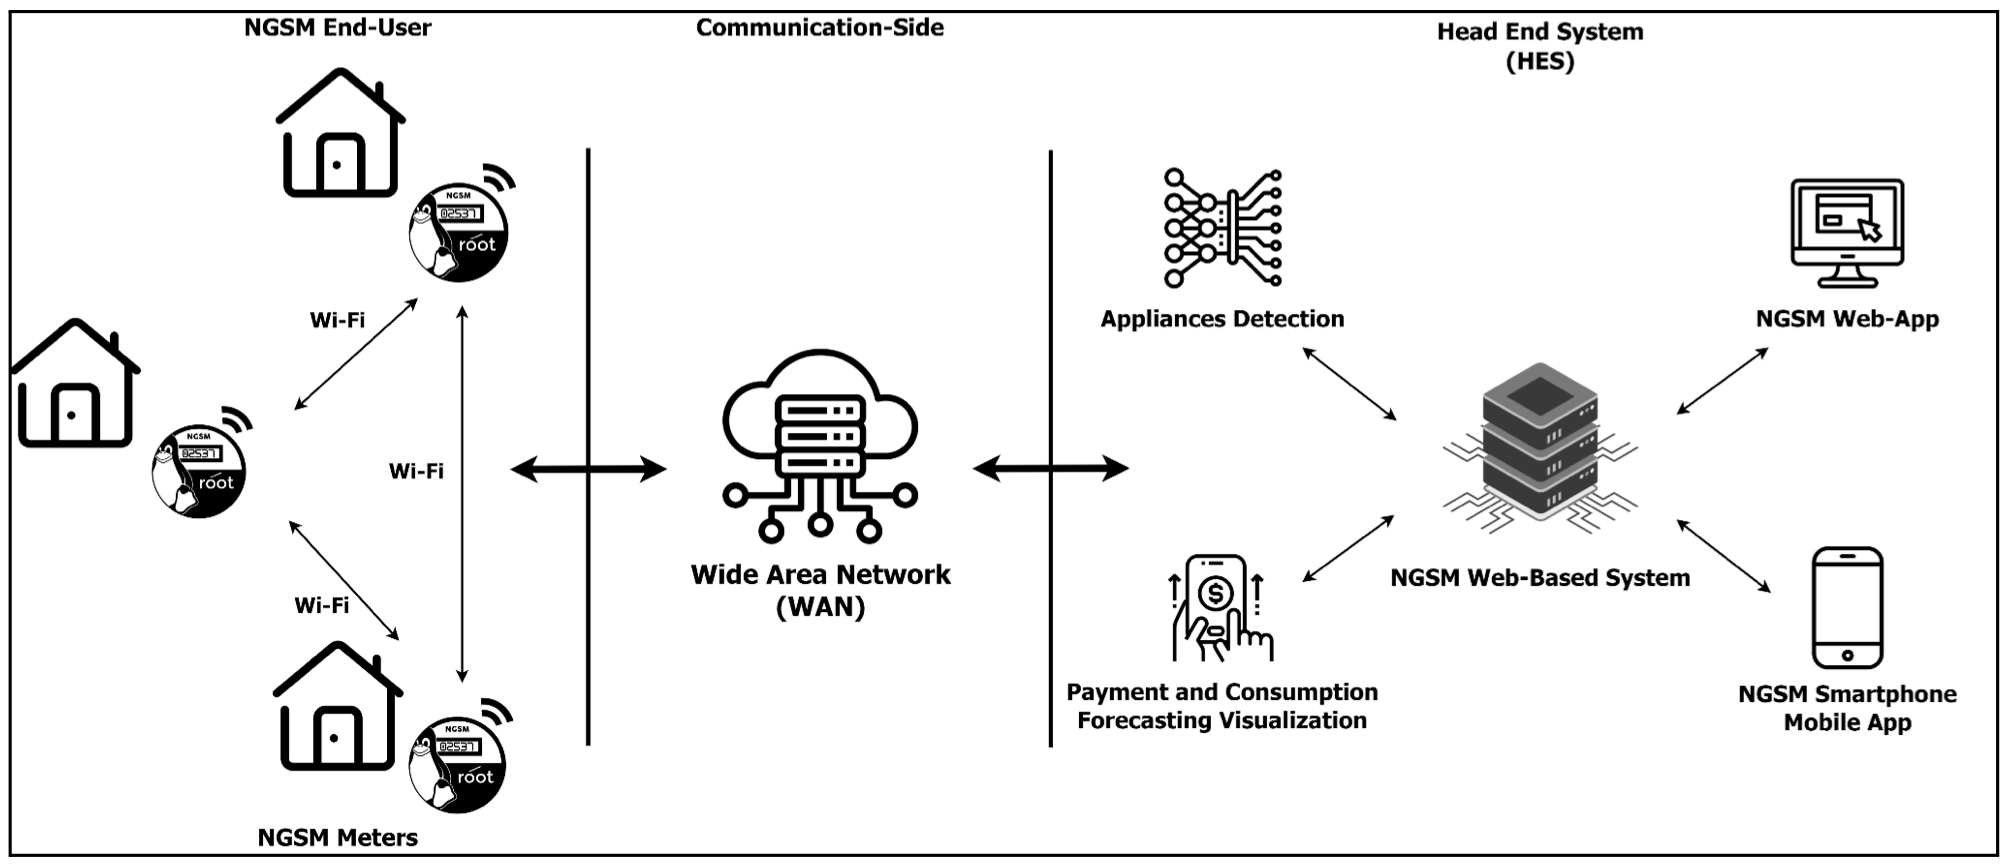
\includegraphics[width=0.90\textwidth]{figures/img1.png}
    \caption{High-level architecture of the NGSM system illustrating the Edge-Cloud data flow.}
    \label{fig:system_arch}
\end{figure}

The fundamental unit of the architecture is the smart meter, which operates as an embedded Linux device integrating software and hardware within a System on Chip (SoC) architecture to support AI-integrated sustainable energy management \cite{ResearchGate2025}. The internal hardware architecture is composed of five critical functional blocks. First, the Analog Front End (AFE) is responsible for the high-frequency acquisition of voltage and current signals, performing Digital Signal Processing (DSP) and electricity tampering detection through live-neutral current comparison \cite{Energize2025}. Second, the Single Board Computer (SBC) hosts the primary SoC, storage, and communication modems, serving as the central processing unit capable of supporting complex AI models. These core elements are supported by a User Interaction module managing the TFT display, a Power Supply unit for regulation, and an Enclosure Tampering Detection system that utilizes electromechanical limit switches to trigger immediate interrupts upon unauthorized disassembly, a critical defense against physical attacks \cite{IJNSA2025}.

Data transmission between the edge nodes and the central infrastructure is mediated by a Wide Area Network (WAN) connecting to the Head-End System (HES). The HES acts as the centralized aggregation point, comprising a web-based dashboard and a smartphone mobile application. Beyond simple data logging, the HES executes high-level administrative tasks including time-of-use (ToU) billing calculation and secure remote payments. Furthermore, it handles advanced visualization by presenting hourly consumption data and appliance-level breakdowns to the consumer, a capability essential for modern utility customer engagement \cite{EY2025}. The HES also serves as the repository for Appliance Detection Analytics, receiving pre-processed classification results from the edge nodes. This strategy of transmitting only inference results rather than raw high-frequency waveforms significantly optimizes network bandwidth and reduces the processing latency typically associated with edge-cloud transfers \cite{MDPI_NILM2025}.


\section{Hardware Implementation}
\label{sec:hardware}

The development of the NGSM hardware followed an iterative engineering methodology, evolving through three distinct generations. This progression was driven by the necessity to balance computational performance for edge-AI tasks against the constraints of power consumption, thermal management, and mass-production viability.

\subsection{First Generation: Proof of Concept}
\label{subsec:gen1}

The initial development phase, designated as the first generation, focused on validating the embedded Linux software stack and the proprietary metrology algorithms without the immediate constraints of power efficiency or industrial form factors. The core processing unit for proof-of-concept prototyping was initially the Raspberry Pi 3 Model B \cite{pi3}, but the benchmarks reported in this study were evaluated on the Raspberry Pi 4 Model B \cite{pi4} to establish a high-performance baseline. This platform features a Quad-core Cortex-A72 (ARM v8) 64-bit SoC clocked at 1.8GHz and 8GB LPDDR4-3200 SDRAM. This high-performance specification provided the necessary computational overhead for compiling the initial C++ daemons and debugging the user-space applications directly on the target device. The utilization of such high-level processors is a documented methodology for rapid prototyping in smart grid applications, allowing developers to isolate algorithmic logic from hardware-level optimization constraints. As illustrated in the hardware block diagram in Figure \ref{fig:gen1_block}, the architecture utilizes the single board computer as the central coordinator for both signal acquisition and user interface management.

\begin{figure}[!t]
    \centering
    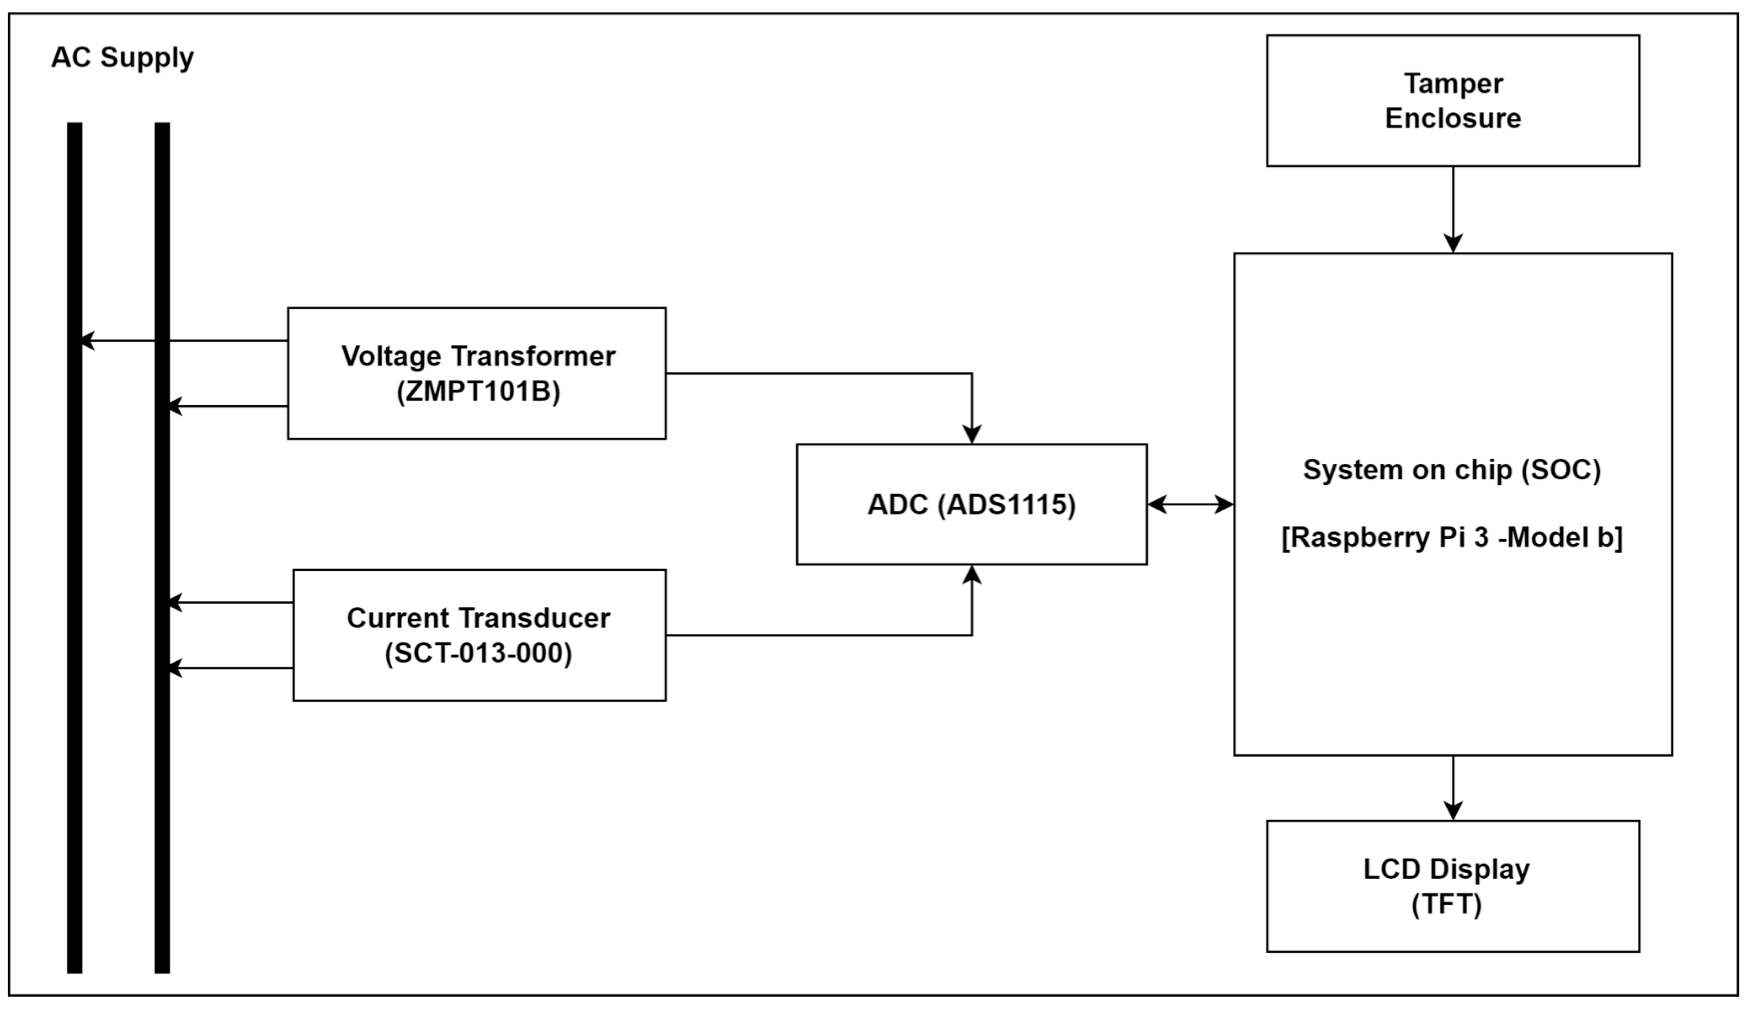
\includegraphics[width=0.90\textwidth]{figures/img3.png}
    \caption{First Generation NGSM Hardware Components illustrating the interface between the Raspberry Pi 3 and discrete analog sensors.}
    \label{fig:gen1_block}
\end{figure}

For the acquisition of electrical parameters, this generation relied on discrete sensing modules rather than an integrated analog front end, a strategy often employed to minimize prototyping costs in real-time energy loggers. Voltage sensing was achieved using the ZMPT101B active single-phase AC voltage sensor \cite{ZMPT101B}. This module utilizes a precision micro-voltage transformer with a 1000:1000 turns ratio and an operational amplifier circuit to step down the 220V grid voltage to a manageable analog signal suitable for digital conversion. Current measurements were performed using the SCT-013-000 split-core current transformer \cite{SCT013401}, a non-intrusive sensor capable of monitoring loads up to 100A with a linearity error of approximately 3 percent.

To verify sensor and peripheral integration during prototyping, real-time voltage and current streams were monitored through the embedded user interface and logging services as well as the working display unit. This verification step confirmed correct signal acquisition and end-to-end data flow prior to calibration and load testing.

With the display and sensor interfaces verified, the focus shifted to the accurate calibration of the load measurement. A critical design challenge with the SCT-013 family is the conversion of the induced secondary current into a voltage signal measurable by the analog-to-digital converter. The transformation ratio is governed by the relationship between the primary and secondary windings as defined in Equation \ref{eq:transformer_ratio}.
\begin{equation}
\label{eq:transformer_ratio}
\frac{I_{secondary}}{I_{primary}} = \frac{N_{primary}}{N_{secondary}}
\end{equation}

Since the SCT-013-100 model lacks an internal burden resistor, an external resistance of 33 Ohms was introduced to the circuit. This resistor converts the secondary current into a voltage drop suitable for the input of the ADS1115 analog-to-digital converter. The relationship between the Root Mean Square current flowing through the load and the peak voltage detected by the sensor is calculated using Equation \ref{eq:peak_voltage}.
\begin{equation}
\label{eq:peak_voltage}
V_{peak} = \sqrt{2} \times I_{RMS(secondary)} \times R_{burden}
\end{equation}
This calibration ensures that for a standard load, the signal remains within the dynamic range of the 16-bit ADS1115, which was interfaced via the I2C bus to digitize the analog waveforms. The physical implementation of the prototype was validated under active load conditions to confirm correct end-to-end sensing and data acquisition prior to extended testing. While this configuration successfully demonstrated the feasibility of the software architecture and edge-processing capabilities, the system exhibited high idle power consumption (523 mA) and significant unit cost, necessitating the subsequent optimization phases.

\subsection{Second Generation: Embedded Optimization and Integrated Metrology}
\label{subsec:gen2}

Following the functional validation of the first generation, the hardware architecture was significantly revised to address two primary deficiencies identified during the proof-of-concept phase: the high idle power consumption (523 mA) of the First Generation quad-core processor and the calibration instability associated with discrete analog sensors. Consequently, the second generation architecture was designed around the Raspberry Pi Zero 2W\cite{RPiZeroW_Datasheet} and the STMicroelectronics STPM33 \cite{STPM33_Datasheet} metering Application Specific Standard Product (ASSP).

The transition to the Raspberry Pi Zero 2W was motivated by the requirement to minimize the thermal footprint and energy overhead of the edge node. Unlike the Raspberry Pi 3 Model B, the Zero 2W employs a Quad-core 64-bit ARM Cortex-A53 processor clocked at 1GHz with 512MB of SDRAM. This architectural reduction results in a 74\% decrease in idle power consumption (134 mA) while retaining sufficient computational capacity for the embedded Linux environment. Furthermore, the inclusion of onboard Wi-Fi (802.11 b/g/n) and Bluetooth in the 'W' model facilitated direct connectivity to the Head-End System without external modems, further reducing the physical footprint of the device. The integration of these components, including the interface between the SoC and the peripheral tampering and display modules, is illustrated in Figure \ref{fig:gen2_hardware}.

\begin{figure}[!t]
    \centering
    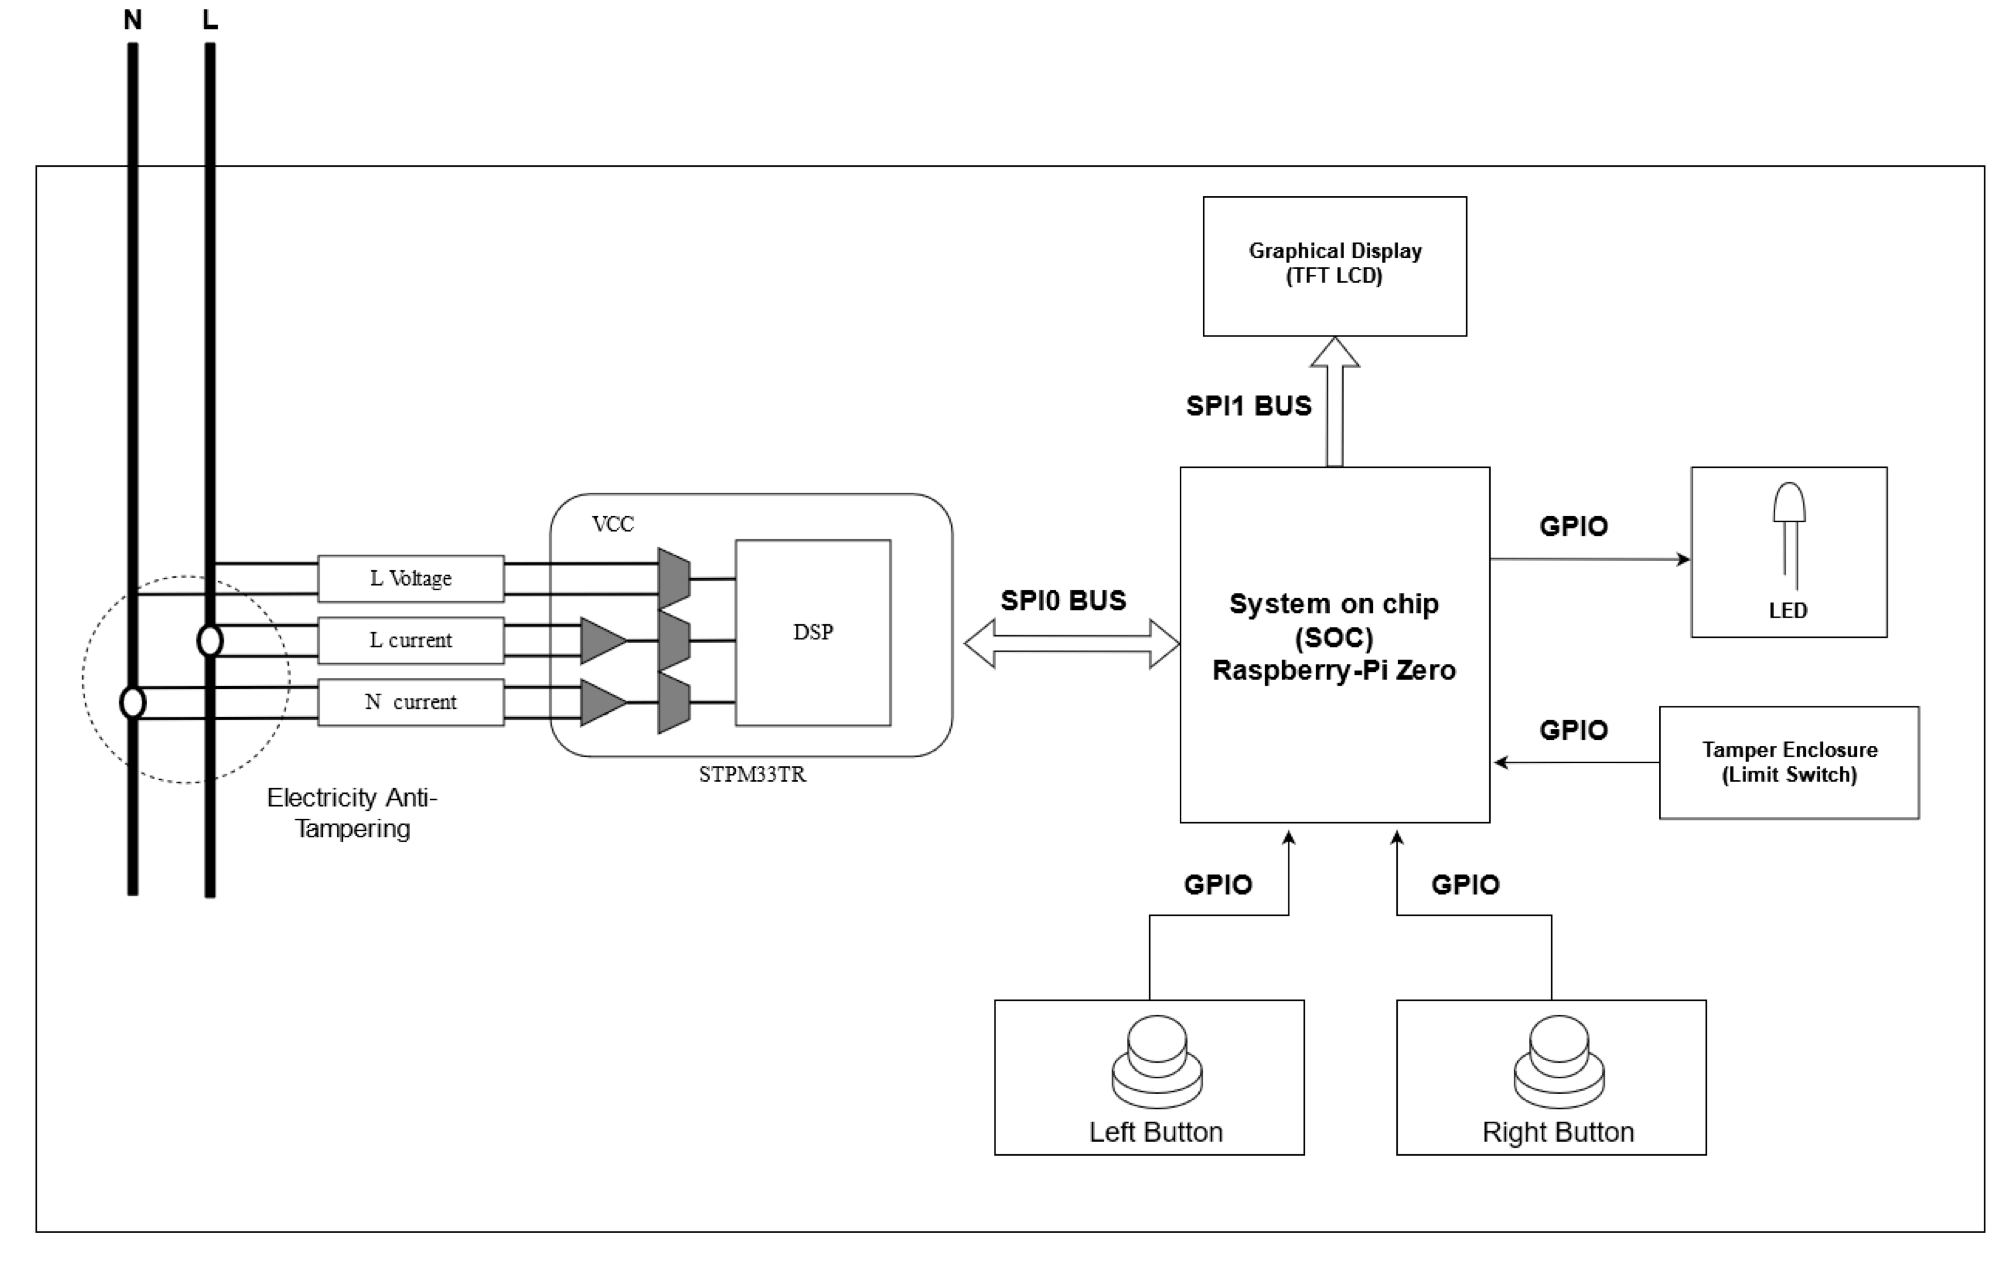
\includegraphics[width=0.90\textwidth]{figures/img7.png}
    \caption{Second Generation NGSM Hardware Components illustrating the integration of the Raspberry Pi Zero 2W with the STPM33 and TFT Display.}
    \label{fig:gen2_hardware}
\end{figure}

Simultaneously, the metrology subsystem was upgraded from discrete transformer-based sensing to a dedicated integrated circuit. The STPM33 was selected for its ability to perform hardware-based calculation of active, reactive, and apparent energy, significantly exceeding the linearity achievable by the previous discrete configuration. The STPM33 interfaces with the host processor via the Serial Peripheral Interface (SPI) bus, which was prioritized over UART to ensure higher data throughput for real-time waveform acquisition. The electrical interface between the grid and the metering IC required specific signal conditioning to match the input dynamic range of the STPM33. Voltage sensing is achieved through a resistive voltage divider network composed of an 810 k$\Omega$ primary resistor (R1) and a 470 $\Omega$ secondary resistor (R2) \cite{EVALSTPM33_UserManual}. To prevent high-frequency noise from corrupting the measurements, an anti-aliasing filter was implemented using a 22 nF capacitor in parallel with the secondary resistor for the voltage channel. Similarly, the current sensing path, driven by Current Transformers (CTs) with a sensitivity of 2.4 mV/A, incorporates a 10 nF capacitor and 1 k$\Omega$ resistors to filter the input signal before digitization \cite{EVALSTPM33_UserManual}. The specific connection topology, utilizing a dual-phase phantom load configuration for calibration and testing, is detailed in Figure \ref{fig:gen2_connection}.

\begin{figure}[!t]
    \centering
    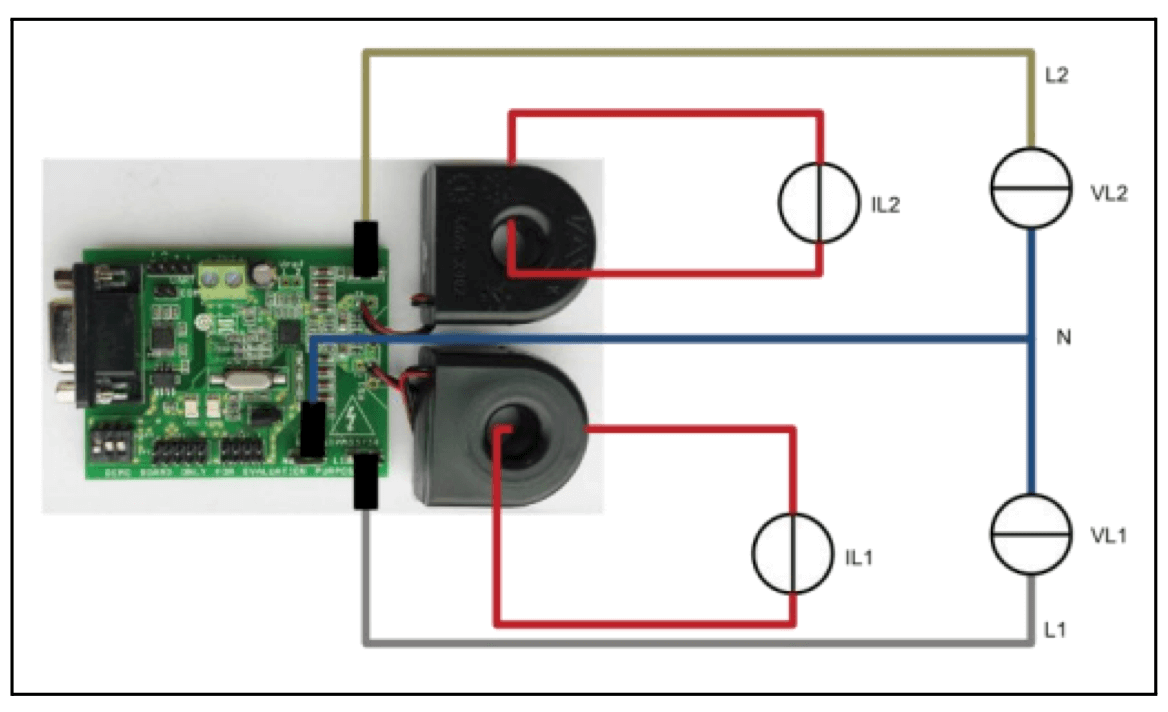
\includegraphics[width=0.50\textwidth]{figures/img8.png}
    \caption{Board connection diagram showing the dual-phase system interface and phantom load configuration.}
    \label{fig:gen2_connection}
\end{figure}

The operational integrity of the second generation was verified through a series of load tests displayed on the integrated TFT panel. Figure \ref{fig:gen2_idle} demonstrates the meter in a quiescent state without an active load, registering a negligible noise floor of 0.014 A, which confirms the effectiveness of the anti-aliasing filters. Conversely, Figure \ref{fig:gen2_load} captures the system accurately measuring a load, registering a current of 0.431 A and a grid voltage of 227.94 V, validating the calibration of the STPM33 DSP unit against the referenced phantom load.

\begin{figure}[!t]
    \centering
    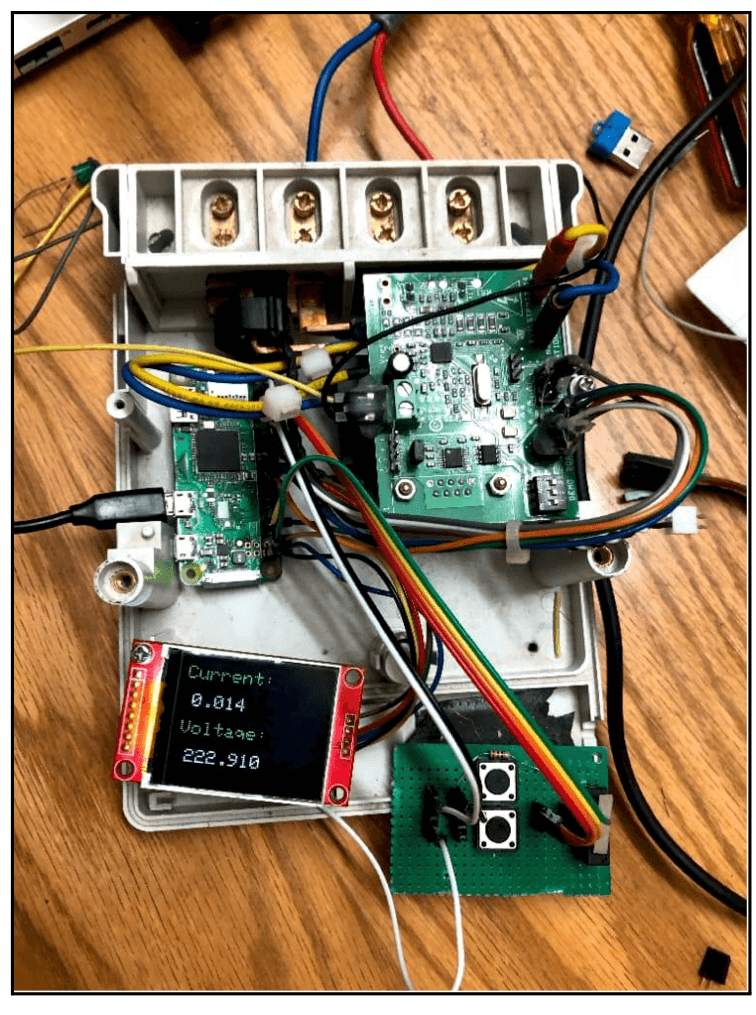
\includegraphics[width=0.48\textwidth]{figures/img9.png}
    \caption{TFT Display output: Measuring without input (Idle state).}
    \label{fig:gen2_idle}
\end{figure}

\begin{figure}[!t]
    \centering
    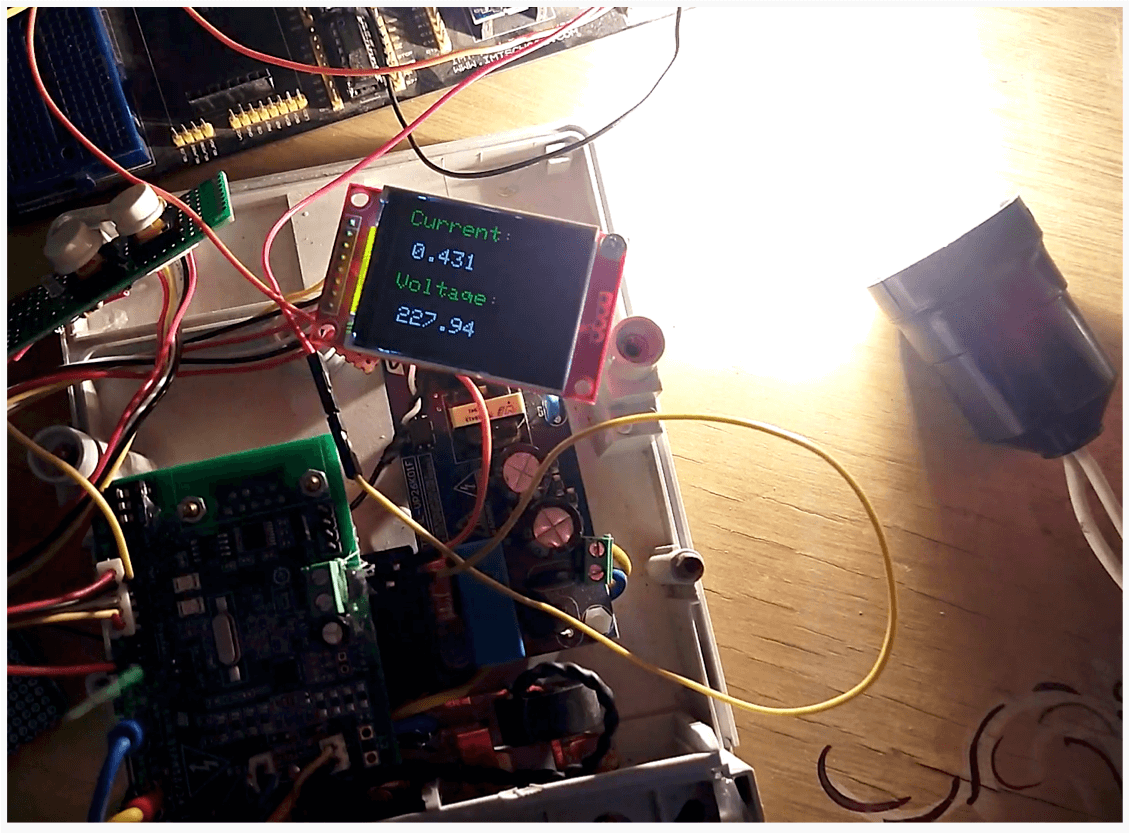
\includegraphics[width=0.50\textwidth]{figures/img10.png}
    \caption{TFT Display output: Measuring active load.}
    \label{fig:gen2_load}
\end{figure}

Figure \ref{fig:gen2_final} presents the final hardware assembly connected to the TFT display, demonstrating the system's compact integration and real-time visualization capabilities. The display interface confirms the correct operation of the metrology unit and the successful boot of the embedded Linux environment on the Raspberry Pi Zero 2W.

\begin{figure}[!t]
    \centering
    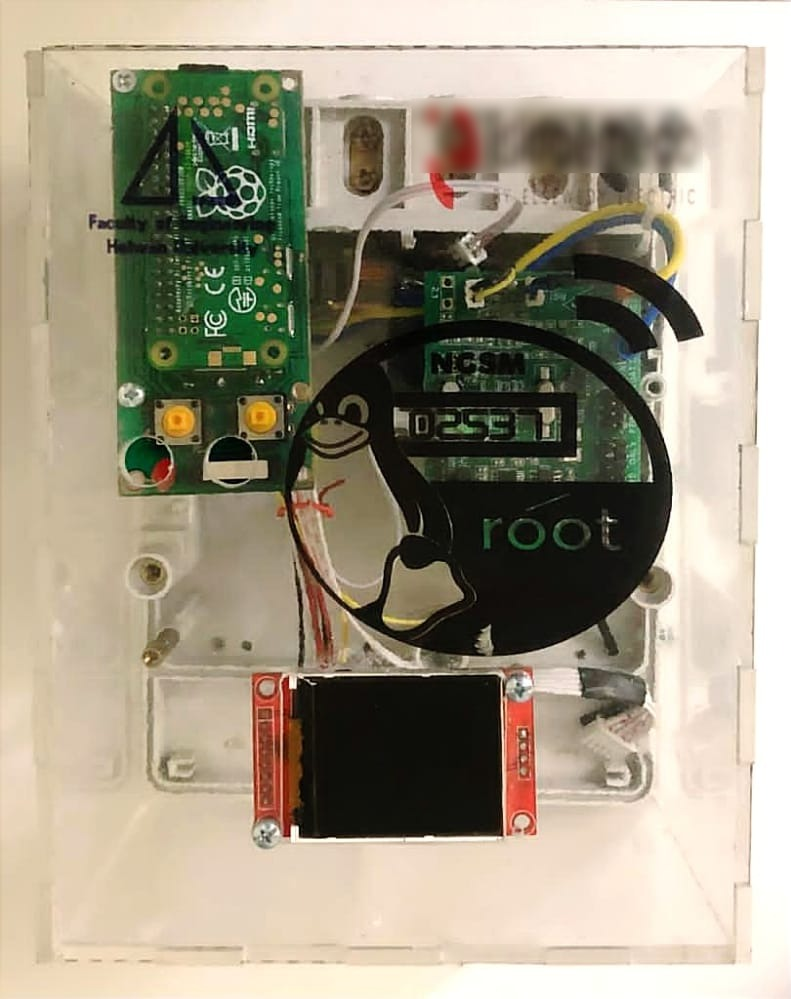
\includegraphics[width=0.48\textwidth]{figures/2ndgen.jpg}
    \caption{Final Second Generation hardware configuration showing the Raspberry Pi Zero 2W connected to the TFT display.}
    \label{fig:gen2_final}
\end{figure}

\subsection{Third Generation: Industrial Scalability and Custom Fabrication}
\label{subsec:gen3}

The third generation of the NGSM architecture was developed to transition the system from a functional prototype to an industrially viable product. This iteration focuses on high-density integration, supply chain independence, and software reliability suitable for mass deployment. The core of this architecture is a custom-fabricated Printed Circuit Board (PCB) design centered around the Allwinner F1C200s System on Chip (SoC) \cite{f1c200s}.

The selection of the Allwinner F1C200s was driven by the necessity for a highly integrated embedded controller capable of supporting multimedia interfaces while maintaining a minimal hardware footprint. The F1C200s (implemented on the MangoPi R3 board \cite{mangopi}) features an ARM926EJ-S core clocked at 420 MHz and integrates 64MB of DDR1 memory directly within the SoC package. This System-in-Package (SiP) design eliminates the need for external RAM modules, significantly reducing the Bill of Materials (BOM) complexity and minimizing trace length susceptibility to electromagnetic interference (EMI) in industrial environments. Furthermore, the SoC natively supports the parallel RGB interface required for the TFT display and the SPI bus for high-speed communication with the metrology unit, allowing for a streamlined hardware topology.

To ensure long-term operational reliability, the storage architecture was migrated from removable SD cards to an onboard SPI NAND Flash memory chip. This change addresses the data integrity risks associated with mechanical contact failure and file system corruption common in consumer-grade storage media. The software environment was strictly optimized through a custom embedded Linux deployment generated via the Buildroot automation system. To utilize the F1C200s effectively, the Device Tree Source (DTS) was manually reconfigured. Conflicting multimedia modules, specifically the LCD controller, TV encoder, and Camera interface, were disabled to release system resources and interrupt lines. This customization enabled the dedication of the high-speed hardware SPI1 controller to the metrology interface on Port E, ensuring reliable communication with the STPM33. Furthermore, the bootloader sequence was customized using U-Boot with specific offsets to support the proprietary partition table. For connectivity, the kernel capabilities were expanded to support USB On-The-Go (OTG) and RNDIS Ethernet gadget modes, facilitating secure local SSH access for system maintenance without requiring external network infrastructure.

As illustrated in Figure \ref{fig:firmware_stack}, this high-efficiency firmware stack separates kernel-space drivers from user-space services. The kernel adheres to a monolithic design where essential drivers are built-in, avoiding the overhead of loadable modules. Core meter functions are implemented as background daemons, specifically utilizing the specialized hardware SPI and GPIO mappings defined in the custom Device Tree to interact with the sensors. Inter-process communication is used to decouple data acquisition from visualization and network tasks, allowing failures in non-critical services to avoid disrupting continuous metrology.

\begin{figure}[!t]
\centering
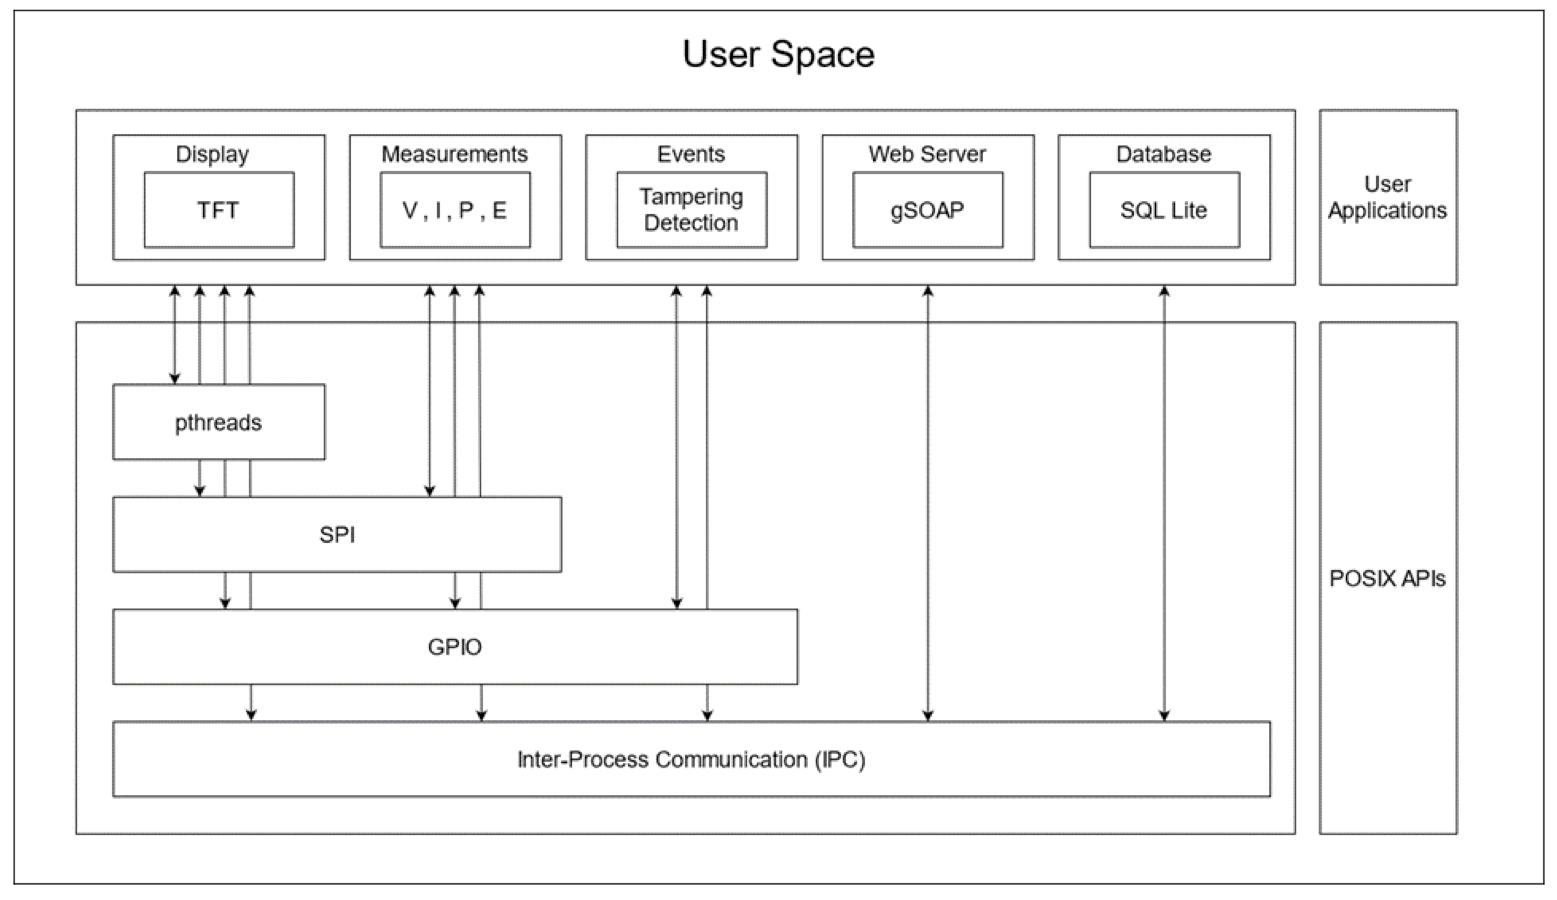
\includegraphics[width=0.90\textwidth]{figures/img2.png}
\caption{Firmware stack illustrating the interaction between User-Space Daemons and Kernel Interfaces via IPC.}
\label{fig:firmware_stack}
\end{figure}


The physical implementation achieves a high degree of miniaturization by integrating the power regulation, metrology, and processing domains onto a single double-layer PCB. As illustrated in Figure \ref{fig:gen3_schematic}, the design leverages the integrated features of the SoC to reduce the peripheral component count.

\begin{figure}[!t]
    \centering
    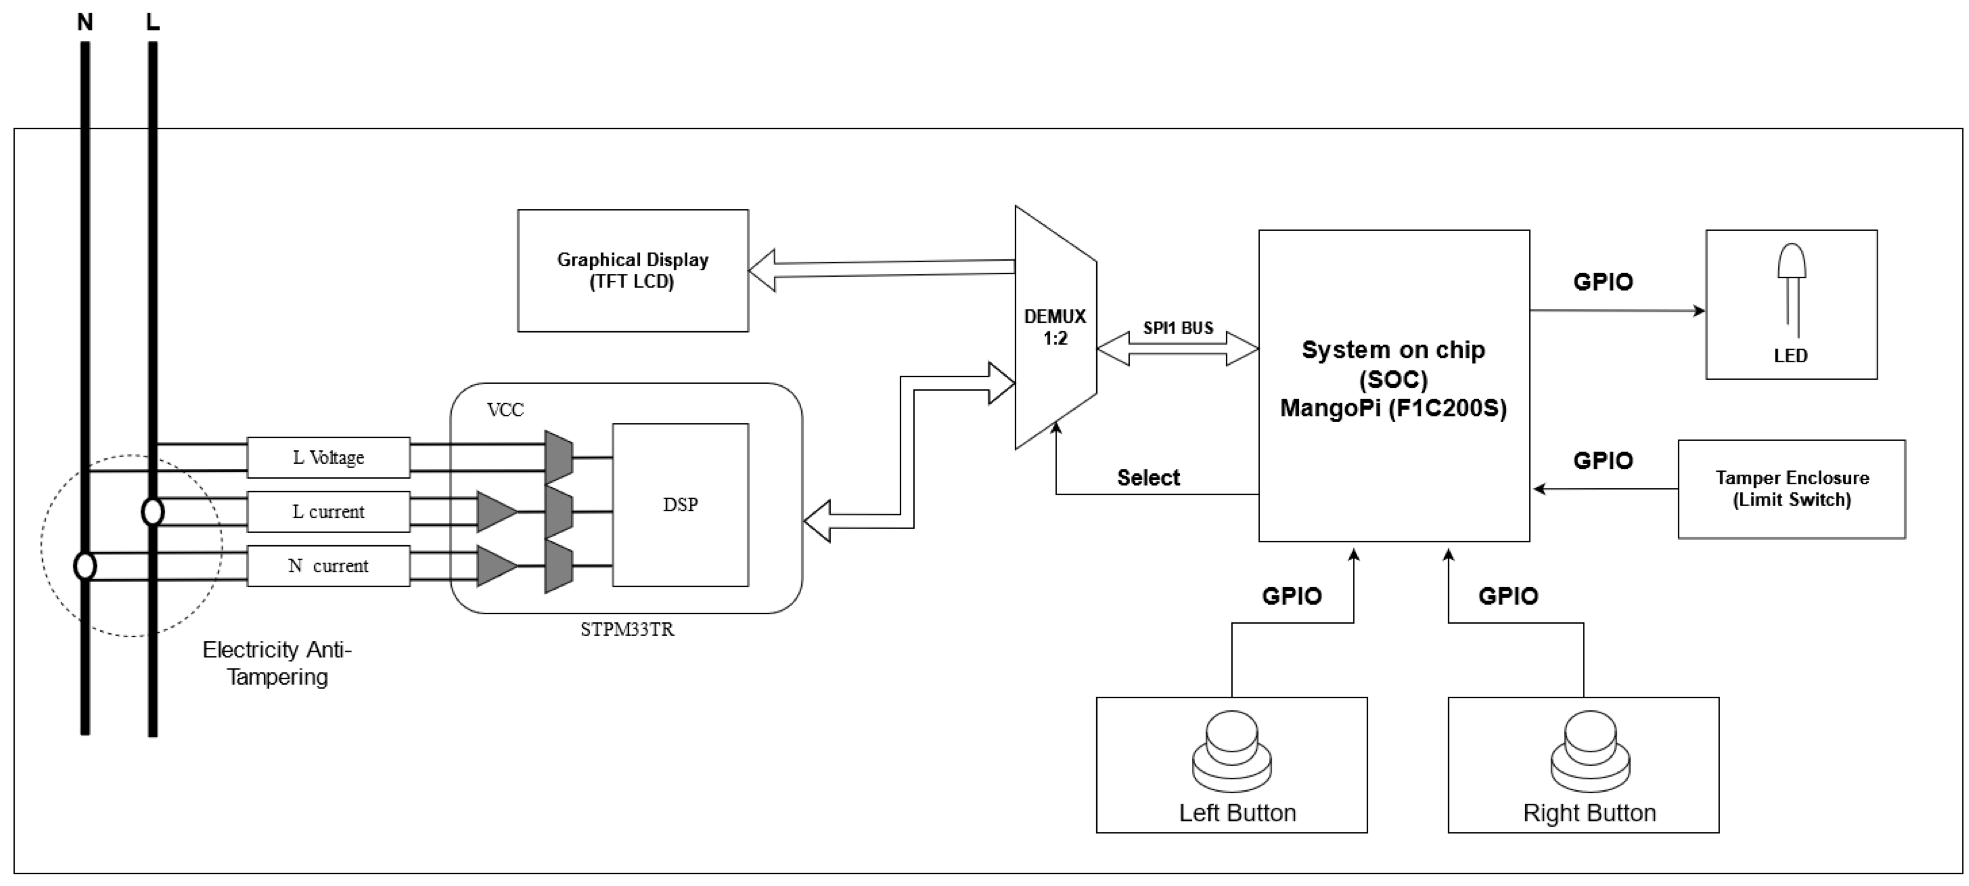
\includegraphics[width=0.95\textwidth]{figures/img11.png}
    \caption{Third Generation NGSM Hardware Components illustrating the schematic integration of the Allwinner F1C200s SoC with the STPM33 and peripheral interfaces.}
    \label{fig:gen3_schematic}
\end{figure}

The layout routes the high-voltage AC inputs and the low-voltage digital signals on isolated planes to maintain signal integrity for the STPM33 analog front end. This consolidated design validates the feasibility of an embedded Linux smart meter capable of advanced edge processing within a form factor compatible with standard industrial enclosures.

\subsection{Performance Benchmarking and Optimization}
\label{subsec:benchmarks}

To quantify efficiency across generations, benchmarks compared First (Raspberry Pi 4 Model B 8 GB RAM), Second (Raspberry Pi Zero 2W 512MB RAM), and Third (MangoPi with Allwinner F1C200s) platforms. All power measurements were recorded at a supply voltage of 5V. As detailed in Table \ref{tab:hardwarebenchmarks}, the evaluation reports idle and active current draw (mA), active CPU load (percentage), and active memory usage (percentage) across hardware generations.

\begin{table*}[!t]
\centering
\caption{Hardware specifications and performance comparison across NGSM generations (Supply Voltage: 5V).}
\label{tab:hardwarebenchmarks}
\small
\begin{tabular}{lcccc}
\toprule
Metric & Gen 1 & Gen 2 & Gen 3 & Improvement (\%) \\
& (RPi 4 Model B) & (RPi Zero 2W) & (MangoPi/F1C200s) & (Gen 2 to Gen 3) \\ \midrule
\multicolumn{5}{l}{Hardware Specifications} \\ 
Processor & Quad Cortex-A72 & Quad Cortex-A53 & Single ARM926EJ-S & -- \\
Clock Speed & 1.8 GHz & 1.0 GHz & 420 MHz & -- \\
Total Memory & 8 GB LPDDR4 & 512 MB SDRAM & 64 MB DDR & -- \\ 
Unit Cost (USD) & 75 & 15 & 16 & -- \\ \midrule
\multicolumn{5}{l}{Measured Performance} \\
Power Idle (mA) & 542.26 & 134.24 & 86.00 & 35.93\% \\
Power Active (mA) & 695.68 & 361.48 & 102.68 & 71.59\% \\
Power Active (W) & 2.71 & 1.81 & 0.513 & 71.59\% \\
CPU Load Active (\%) & 75.35 & 75.29 & 84.31 & N/A \\
Memory Usage Active (\%) & 5.00 & 43.91 & 48.92 & N/A \\ \bottomrule
\multicolumn{5}{l}{\footnotesize Notes: Unit cost refers to retail development board price. F1C200s SiP component cost: \$3-5 in volume.} \\
\multicolumn{5}{l}{\footnotesize Active and idle power measurements were taken under comparable benchmarking workloads.} \\
\multicolumn{5}{l}{\footnotesize Power (W) calculated as: current (mA) × voltage (5V) / 1000.}
\end{tabular}
\end{table*}

\section{Software Components}
\label{sec:software}

\subsection{Web-Based System Architecture}
\label{subsec:web_arch}

The fundamental communication topology is defined by the interaction between the edge nodes and the central cloud infrastructure. As illustrated in Figure \ref{fig:system_block}, the system connects the NGSM meters via a Wide Area Network (WAN) to a centralized Head-End System (HES). This aggregation point manages critical utility functions, including appliance detection analytics, consumption forecasting, and secure payment processing. The architectural decision was made to decouple the visualization logic from the metrological acquisition, ensuring that heavy query loads from user applications do not degrade the real-time performance of the edge metering services \cite{8849012, Bera2014}.

\begin{figure}[!t]
    \centering
    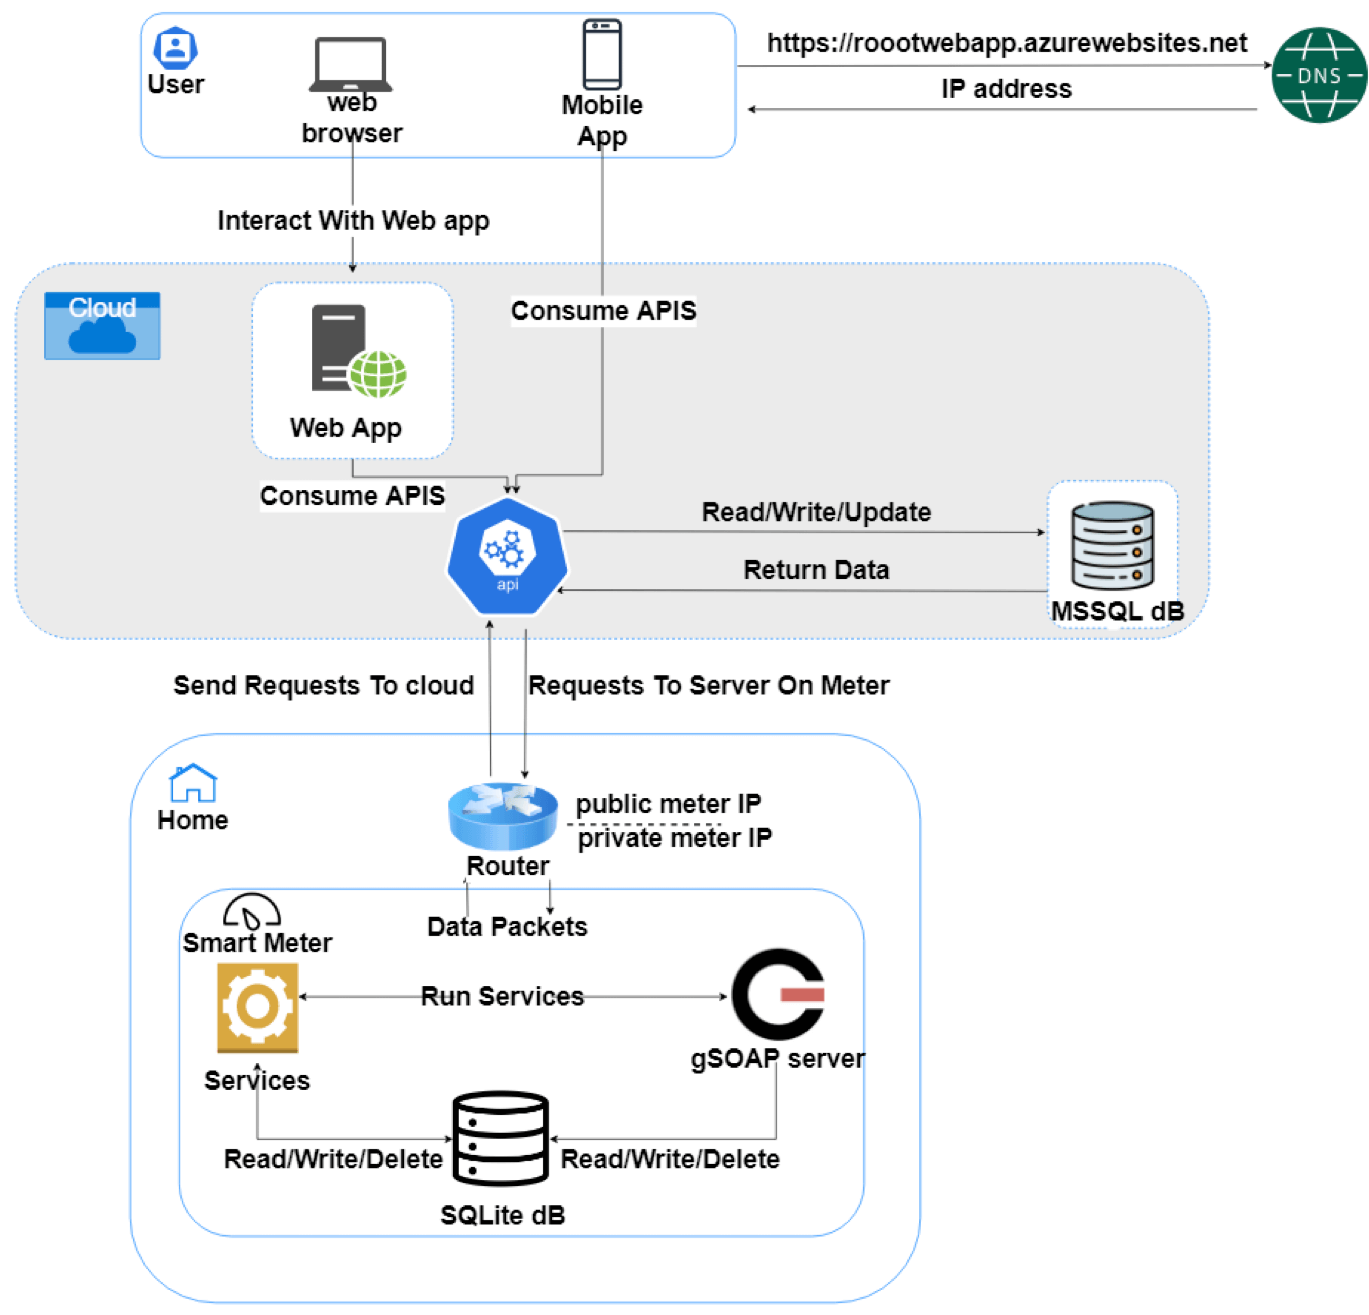
\includegraphics[width=0.90\textwidth]{figures/img12.png}
    \caption{NGSM System Block Diagram illustrating the data flow between Edge Nodes, WAN, and the Head-End System services.}
    \label{fig:system_block}
\end{figure}

The detailed software stack, depicted in Figure \ref{fig:web_arch}, relies on a service-oriented architecture (SOA) to handle the diverse data streams. On the cloud side, the backend is structured around a suite of specialized Application Programming Interfaces (APIs). These include the Meter API for receiving raw voltage and current payloads, the Consumption API for historical data aggregation, and the Event API for high-priority interrupt logging, such as tampering alerts. Financial transactions are managed through a dedicated Payment API integrated with the Stripe gateway, while a Bill API dynamically generates invoices based on accumulated consumption records stored in an MSSQL relational database. The reliability of this distributed communication network was designed to withstand the latency and packet loss typical of smart grid environments \cite{Patel2024}.

\begin{figure}[!t]
    \centering
    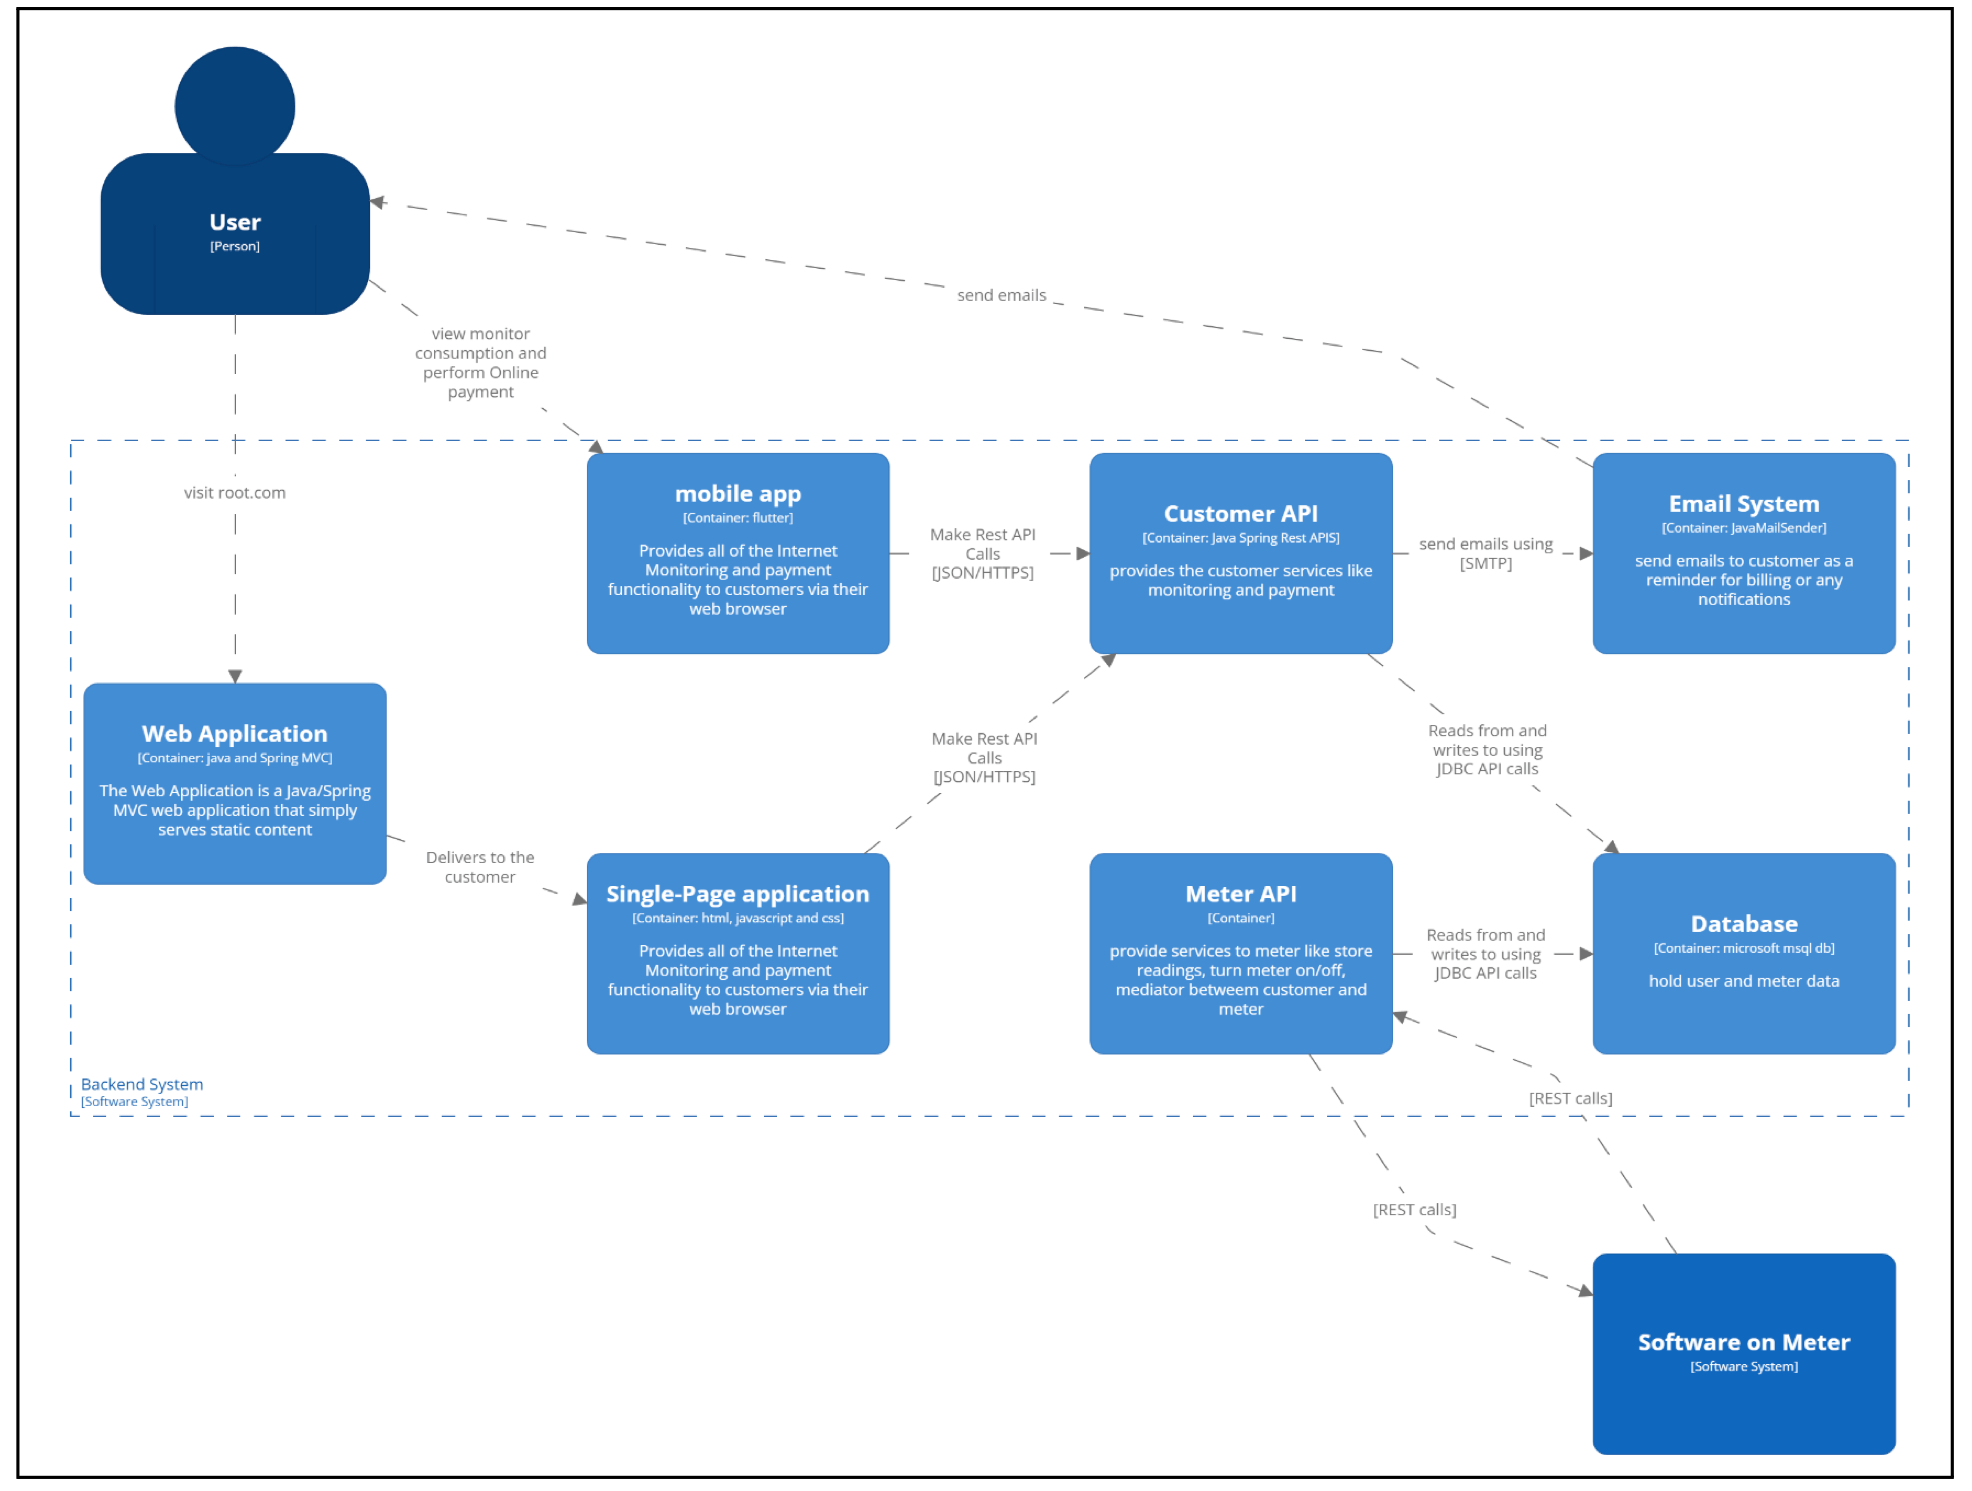
\includegraphics[width=0.90\textwidth]{figures/img13.png}
    \caption{Detailed NGSM Web-Based System Architecture showing the API interaction between the Meter Firmware, Cloud Backend, and Client Applications.}
    \label{fig:web_arch}
\end{figure}

Conversely, the meter-side software is engineered to operate within the constrained resources of the Allwinner F1C200s. To achieve this, the local web server implementation utilizes lighttpd, selected for its minimal memory footprint and superior request handling capabilities compared to standard Apache deployments in IoT contexts \cite{Babovic2016}. The communication layer is implemented in C++ using the gSOAP toolkit, which provides a lightweight XML data binding mechanism for handling SOAP/REST web services \cite{Engelen2002}. This native C++ implementation ensures that the overhead of network serialization does not impede the high-frequency sampling required by the metrology thread.

\subsection{Client-Side Web Application}
\label{subsec:webapp}

The consumer-facing component of the Head-End System was developed as a comprehensive Single Page Application (SPA) utilizing the ReactJS framework. This architectural choice was driven by the necessity for a high-performance, component-based interface capable of rendering dynamic energy data without the latency associated with traditional server-side page reloads. Comparative studies indicate that ReactJS offers superior state management for live dashboards through its Virtual DOM implementation, a critical factor for maintaining user engagement in real-time monitoring systems where data freshness is paramount \cite{Chopra2021_FlaskReactDashboard}. The application hosting is managed via the Microsoft Azure cloud platform, ensuring high availability and scalable load balancing for the static frontend assets.

The navigational structure of the application is rigorously architected to enforce security and access control. As illustrated in the user flow diagram in Figure \ref{fig:user_flow}, the routing logic distinguishes between public "landing" zones and secured private routes. Access to sensitive dashboard modules is guarded by a client-side authentication handler that verifies JSON Web Tokens (JWT) issued by the backend upon successful login. This separation ensures that unauthenticated requests are intercepted at the routing level, preventing unauthorized access to personal consumption data or payment gateways.

\begin{figure}[!t]
    \centering
    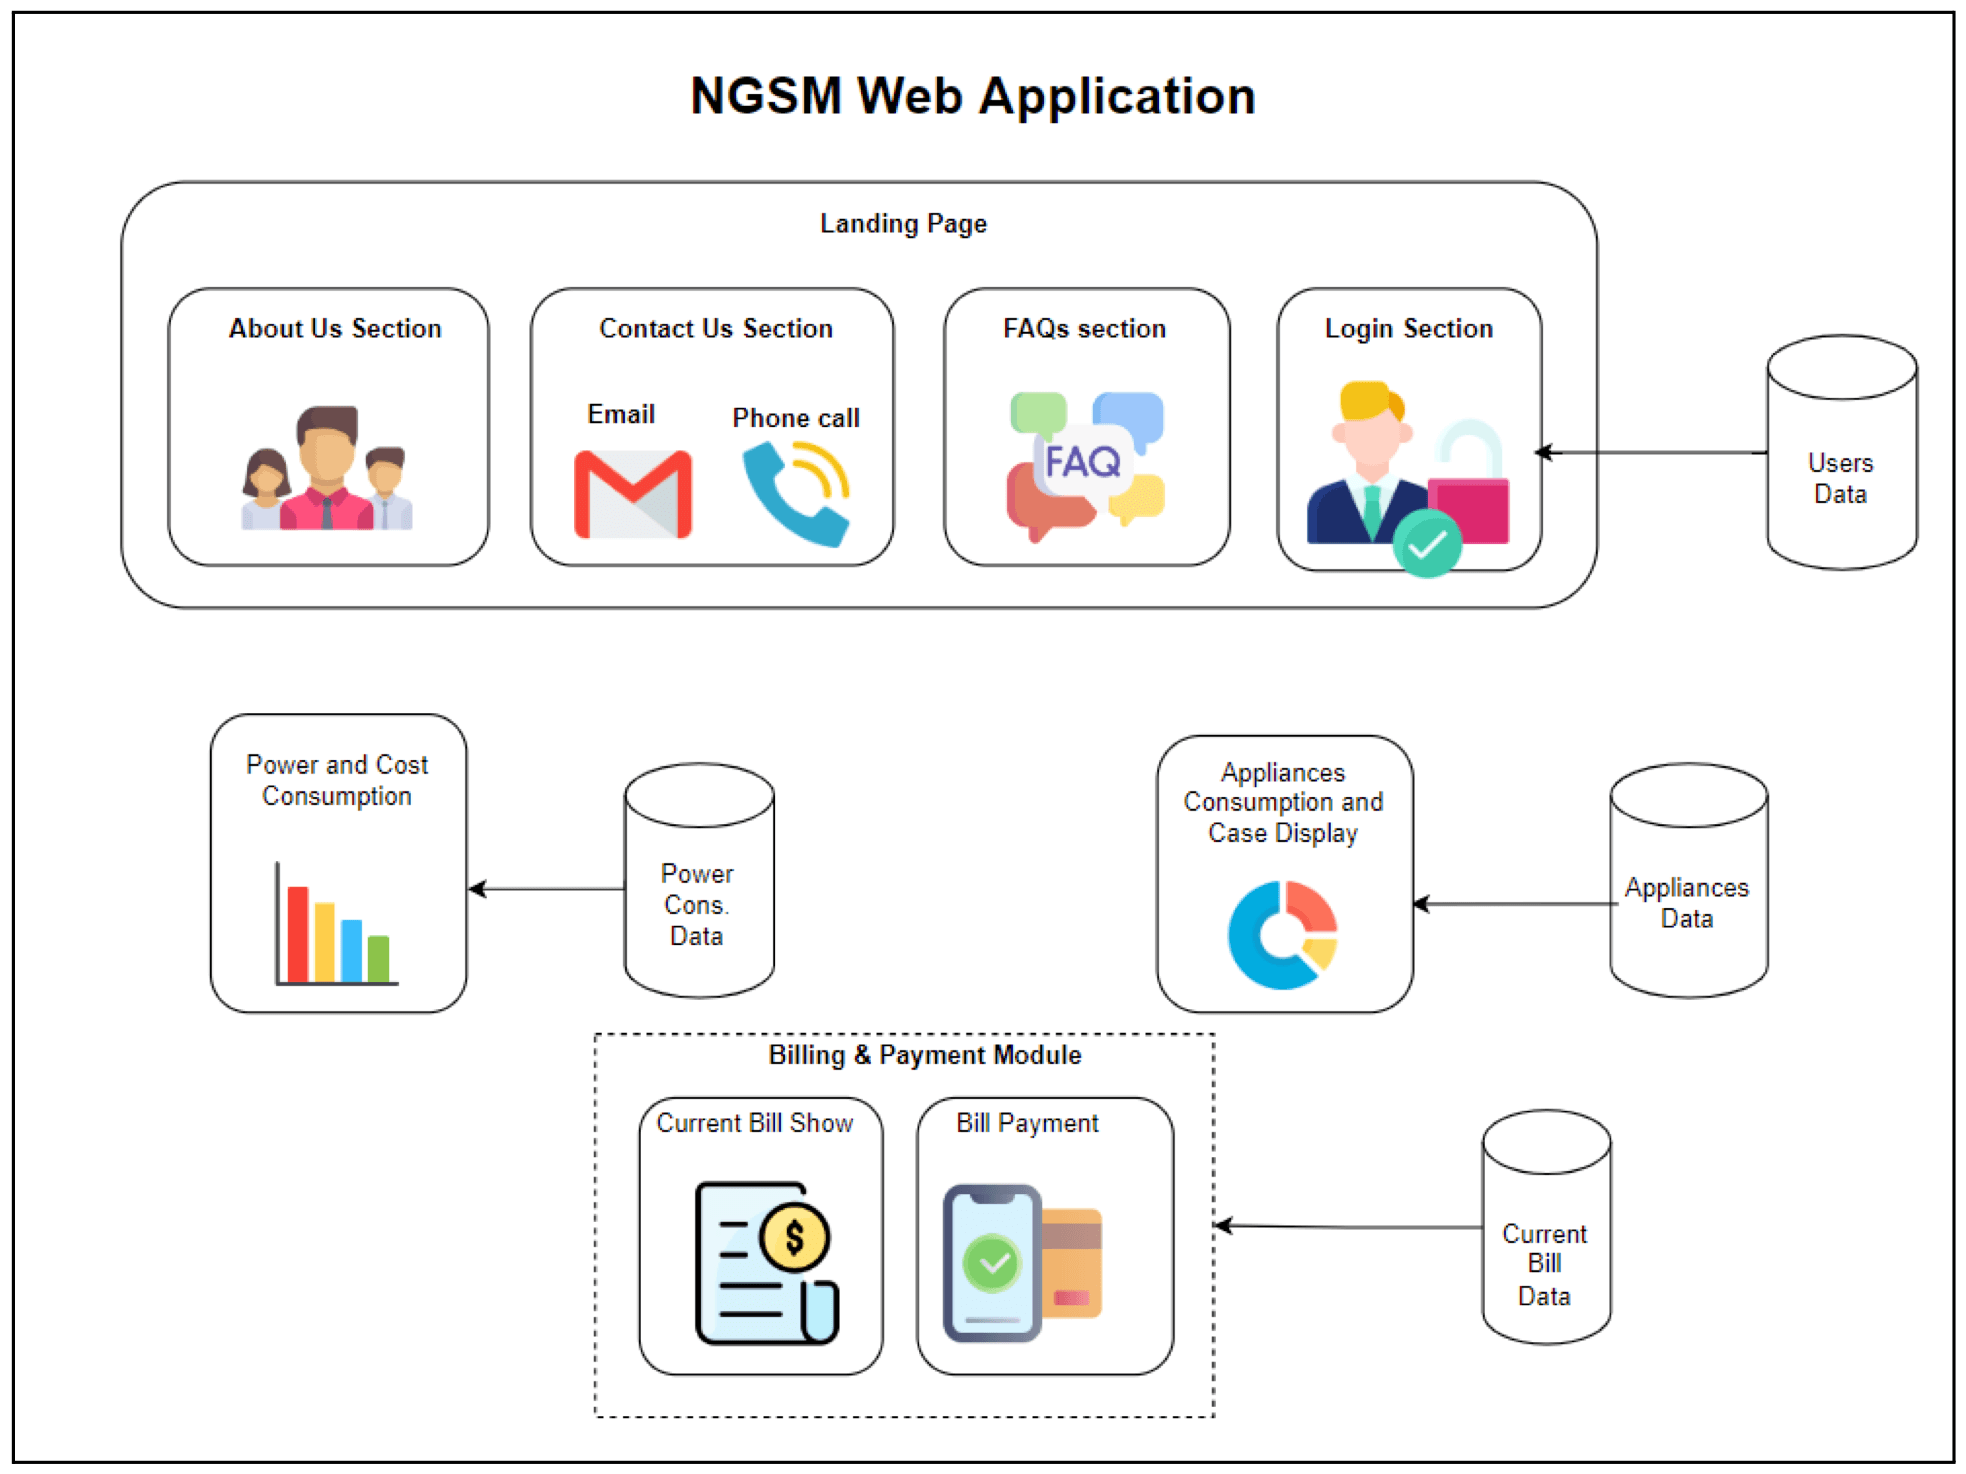
\includegraphics[width=0.85\textwidth]{figures/img14.png}
    \caption{User Interaction Flow Diagram illustrating the navigation paths between public pages, authentication layers, and private dashboard modules.}
    \label{fig:user_flow}
\end{figure}

Upon accessing the platform, the user interface presents a modular informational layer designed to facilitate self-service support. To mitigate the operational burden on utility support staff, a comprehensive Frequently Asked Questions (FAQ) module was integrated directly into the primary navigation bar. This FAQ interface uses an accordion-style layout to organize common queries regarding billing cycles, meter installation procedures, and account management. This immediate access to troubleshooting information allows users to resolve standard inquiries independently, thereby reducing the volume of support tickets generated for the utility provider.

The central analytical feature of the application is the Consumption Dashboard, which visualizes the telemetry data aggregated by the NGSM meters. This module, depicted in Figure \ref{fig:consumption_page}, communicates with the cloud Consumption API to retrieve historical usage datasets filtered by user-defined date ranges. The raw data is processed client-side and rendered into interactive bar charts and numerical summaries, providing users with granular visibility into their electrical expenditure and accumulated costs. Academic research suggests that such interactive visualizations are essential for triggering the behavioral changes necessary for sustainable energy consumption, as they translate abstract kilowatt-hour metrics into actionable financial insights \cite{mti3030056}.

\begin{figure}[!t]
    \centering
    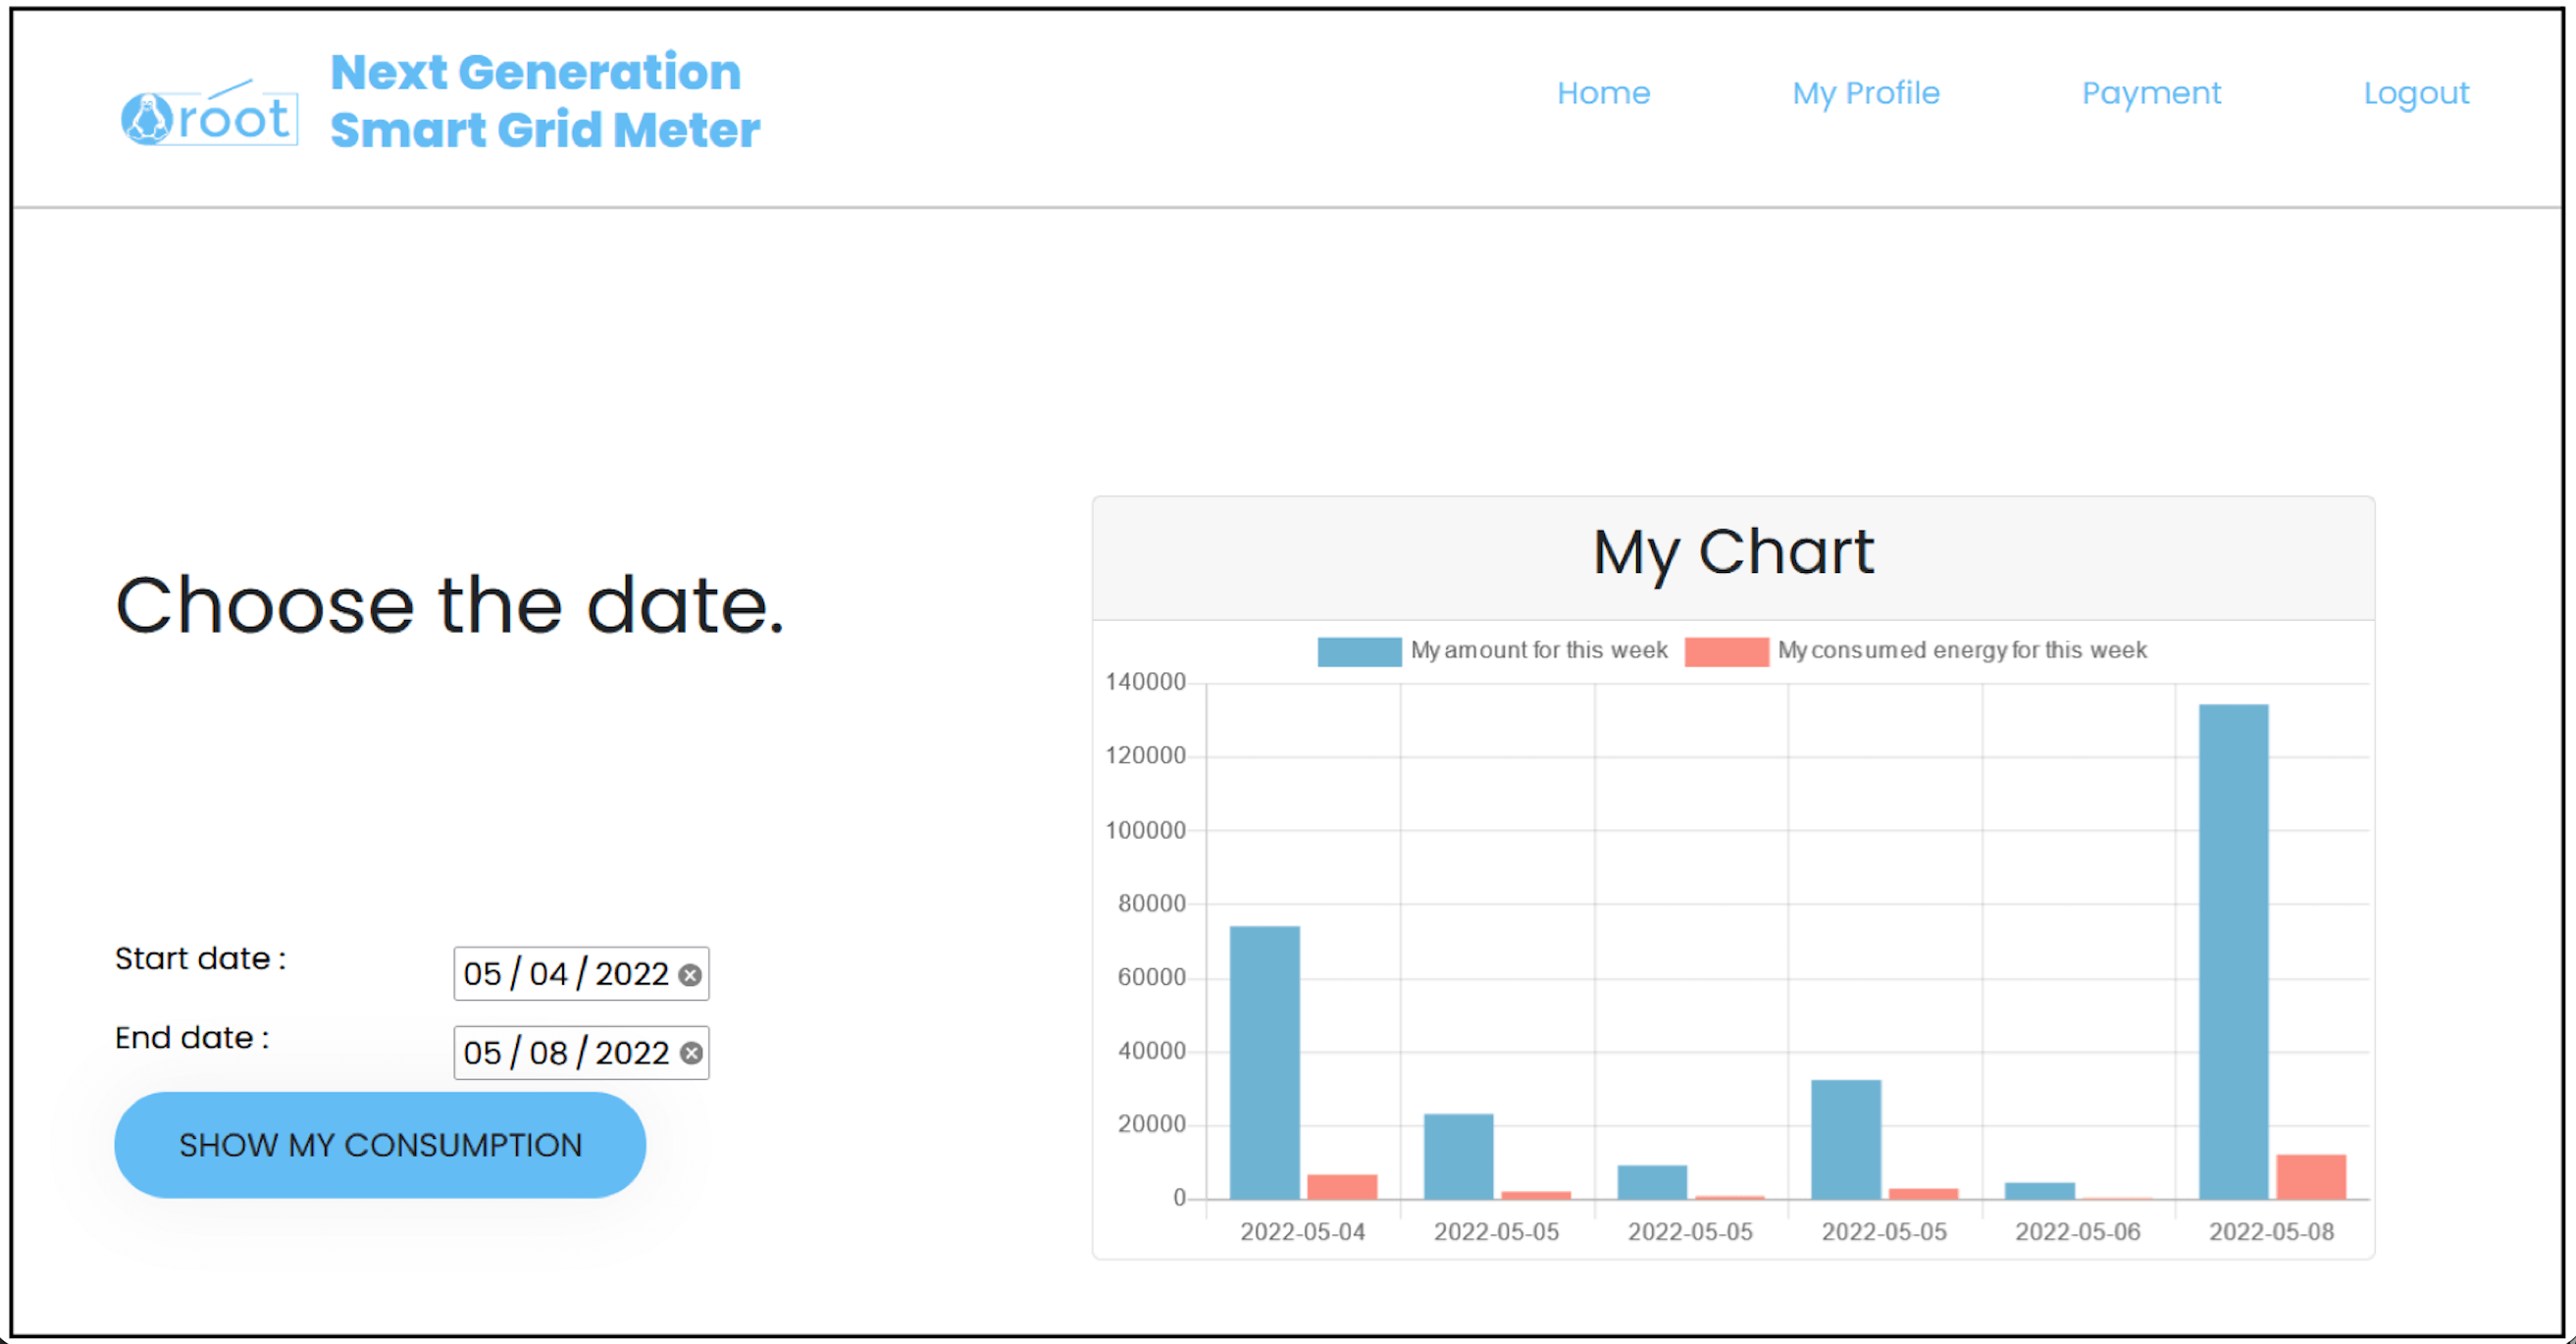
\includegraphics[width=0.85\textwidth]{figures/img16.png}
    \caption{Energy Consumption Dashboard providing visualization of historical usage and cost metrics.}
    \label{fig:consumption_page}
\end{figure}

Financial settlement is managed through a secure Payment and Billing module. This interface integrates the Stripe payment gateway API to process credit card transactions while maintaining strict PCI-DSS compliance. By offloading the tokenization of sensitive financial credentials to the Stripe service, the utility avoids storing credit card details on its own servers. A secure payment interface is implemented to display the outstanding balance and billing period and to provide a secure input form for transaction completion. The integration ensures that payment confirmations are instantaneously reflected in the user's account status via synchronous callback hooks from the (Payment API).

\subsection{Cross-Platform Mobile Application}
\label{subsec:mobileapp}

Complementing the web-based interface, a dedicated mobile application was developed to provide users with ubiquitous access to their energy telemetry. The application was built using the Flutter framework and the Dart programming language. This technology stack was selected for its ability to compile a single codebase into native binaries for both Android and iOS platforms. Comparative studies indicate that Flutter provides superior rendering performance and consistency across different operating systems compared to alternative cross-platform frameworks, significantly reducing the development overhead while maintaining native-level responsiveness \cite{Gülcüoğlu2021}. The application architecture strictly follows the interaction flow defined in Figure \ref{fig:mobile_activity}, ensuring that all data requests are authenticated against the Head-End System APIs before displaying sensitive consumption or billing information.

\begin{figure}[!t]
    \centering
    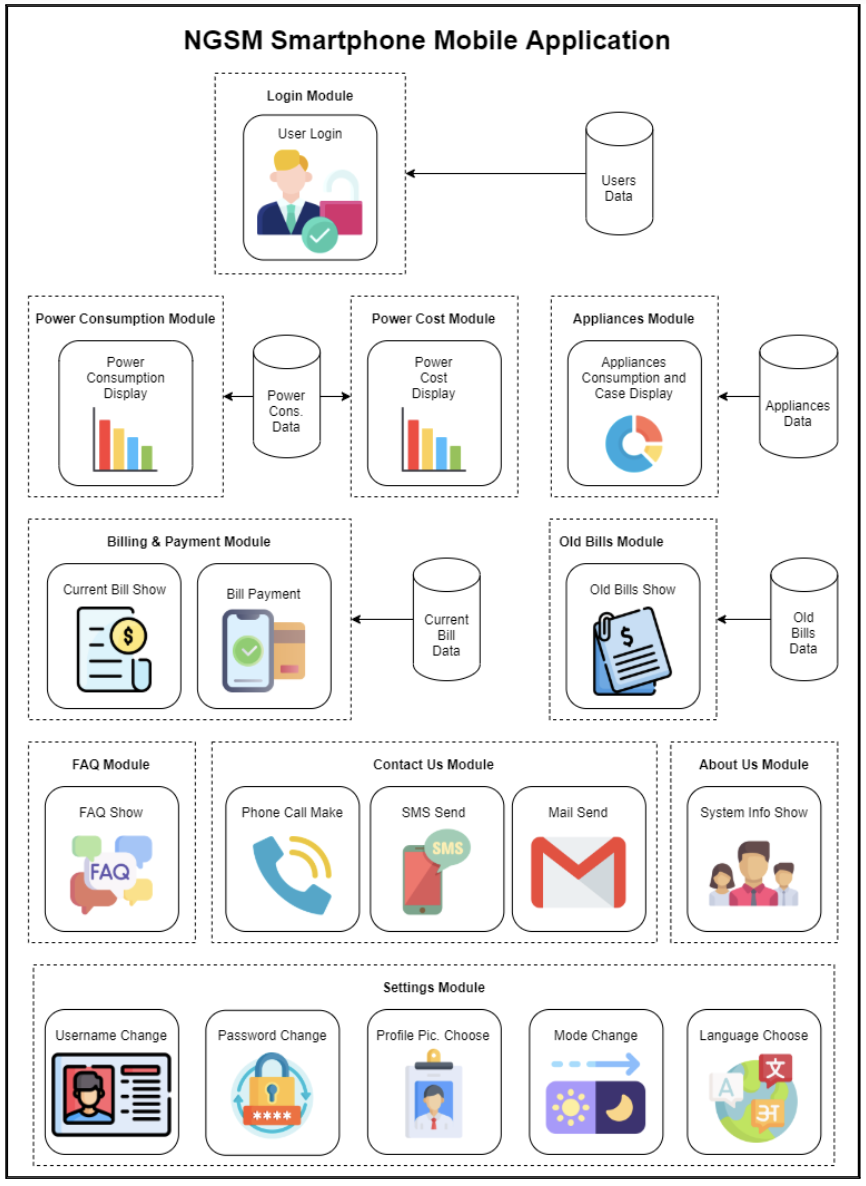
\includegraphics[width=0.50\textwidth]{figures/img18.png}
    \caption{Activity Diagram illustrating the operational flow of the NGSM Mobile Application.}
    \label{fig:mobile_activity}
\end{figure}

The user experience is anchored by a secure authentication layer. Upon launching the application, users are presented with a login interface that secures access using the same credentials as the web platform. To ensure account accessibility, the system includes a dedicated credential recovery flow that enables password reset without requiring administrative intervention.

The core utility of the application lies in its ability to visualize both physical energy usage and the associated financial impact. A dedicated analytics module allows users to toggle between these two critical views. As depicted in Figures \ref{fig:mobile_kwh} and \ref{fig:mobile_cost}, the application renders the aggregated load data in kilowatt-hours (kWh) and the corresponding monetary cost in the local currency. This dual visualization enables users to correlate their daily activities directly with their electricity expenditure. Systematic reviews of residential energy behavior have demonstrated that such mobile-based feedback interfaces are effective tools for promoting energy conservation and sustaining long-term behavioral change \cite{chatzigeorgiou2021}.

\begin{figure}[!t]
    \centering
    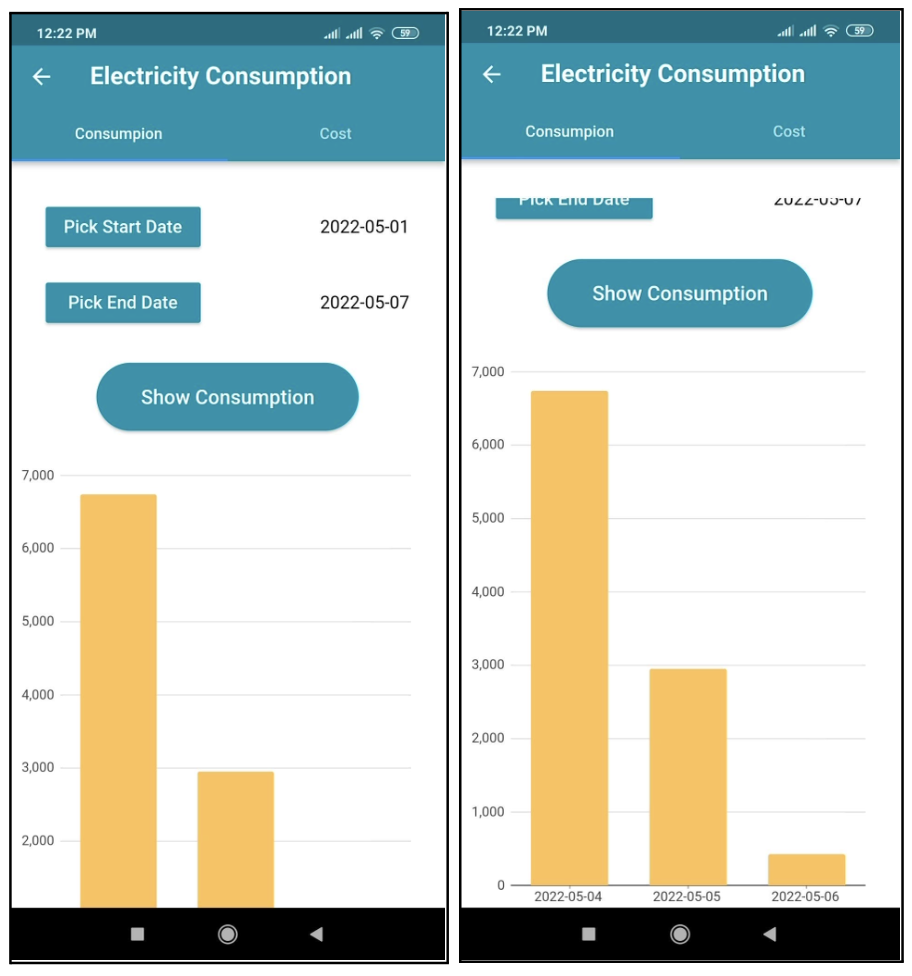
\includegraphics[width=0.50\textwidth]{figures/img21.png}
    \caption{Energy Consumption (kWh) View.}
    \label{fig:mobile_kwh}
\end{figure}

\begin{figure}[!t]
    \centering
    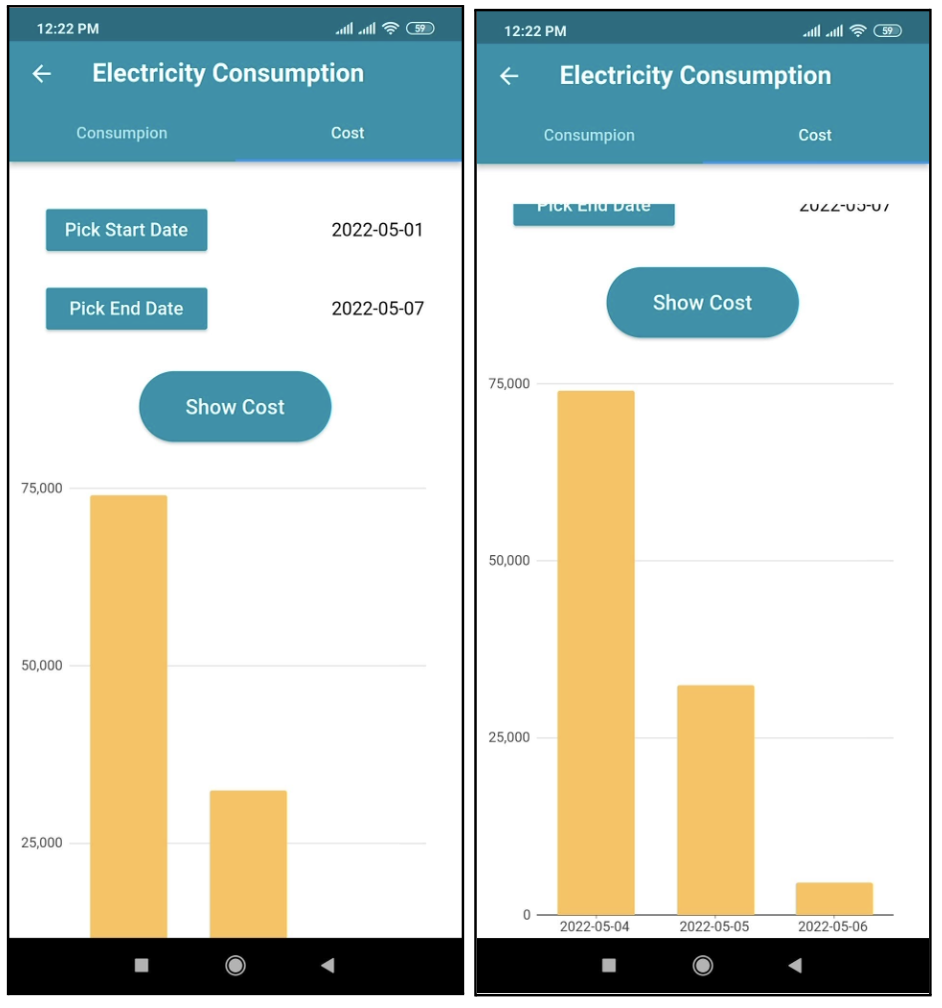
\includegraphics[width=0.50\textwidth]{figures/img22.png}
    \caption{Calculated Cost View.}
    \label{fig:mobile_cost}
\end{figure}

Administrative tasks are handled through the billing and payment modules. The application generates a digital invoice that summarizes the total consumption and cost for the current billing cycle. To support financial tracking, the system maintains a historical repository of previous invoices, allowing past payments to be reviewed and long-term billing trends to be monitored within the application interface.

A distinguishing feature of the NGSM mobile application is the real-time visualization of Appliance Detection results. Leveraging the Non-Intrusive Load Monitoring (NILM) analytics processed by the edge node, the application displays a live status dashboard for major household appliances. Each detected device is represented with its current operational state (ON/OFF) and instantaneous power draw. This granular visibility empowers consumers to identify and isolate high-consumption devices, bridging the gap between aggregate meter readings and specific appliance usage.

\section{Advanced Data Analytics and ML/DL Techniques}
\label{sec:ai}

This section presents the advanced analytics capabilities integrated into NGSM, focusing on algorithms that can be executed close to the measurement source under the latency, privacy, and resource constraints of smart metering deployments. Building on the embedded hardware and software stack described earlier, the proposed analytics pipeline performs local signal analysis for power-quality monitoring and supports intelligent load understanding through Non-Intrusive Load Monitoring (NILM). In addition to real-time edge operation, the section introduces a training and adaptation methodology that enables robust performance across heterogeneous households while preserving data locality through privacy-aware learning mechanisms.


\subsection{Power Quality and Harmonic Analysis}
\label{subsec:harmonics}

Power quality health serves as a fundamental indicator of electrical system stability. In modern distribution networks, the proliferation of non-linear loads such as Switch-Mode Power Supplies (SMPS), Variable Frequency Drives (VFDs), and household electronics has introduced significant challenges to maintaining a sinusoidal waveform \cite{dugan2012electrical}. These loads draw non-sinusoidal currents, resulting in harmonic distortions that can lead to equipment overheating, neutral conductor overloading, and mechanical resonance in transformers. Recent studies emphasize the necessity of robust classification methods to identify these disturbances early and prevent long-term infrastructure damage \cite{eristi2022new}. Consequently, the ability to detect and quantify these disturbances at the grid edge is a critical function of the NGSM system. Harmonics are defined as voltage or current components operating at frequencies that are integer multiples of the fundamental system frequency. According to Fourier's theorem, any periodic non-sinusoidal waveform can be decomposed into the summation of a DC component, a fundamental sine wave, and a series of higher-order harmonic frequencies. The instantaneous signal $y(t)$ is modeled as shown in Equation \ref{eq:fourier}:

\begin{equation}
\label{eq:fourier}
y(t) = Y_0 + \sum_{h=1}^{\infty} Y_h \sqrt{2} \sin(h\omega t - \phi_h)
\end{equation}

Where $Y_0$ represents the DC component, $Y_h$ is the Root Mean Square (RMS) value of the harmonic at order $h$, $\omega$ is the angular frequency of the fundamental component, and $\phi_h$ is the phase displacement \cite{wakileh2001power}.

To quantify the severity of the waveform distortion, the Total Harmonic Distortion (THD) metric is utilized. This indicator expresses the ratio of the RMS value of all harmonic components to the RMS value of the fundamental frequency, calculated via Equation \ref{eq:thd}:

\begin{equation}
\label{eq:thd}
THD = \frac{\sqrt{\sum_{h=2}^{H} Y_h^2}}{Y_1}
\end{equation}

The NGSM architecture implements a distributed detection strategy that processes these waveforms directly at the meter node. By utilizing the high-frequency sampling capabilities of the metrology unit, the embedded firmware executes a Fast Fourier Transform (FFT) to extract the spectral composition of the voltage and current signals. This approach aligns with modern distributed edge computing paradigms, which prioritize local data processing to achieve efficient and adaptable grid management without incurring the latency associated with centralized cloud analysis \cite{shang2021achieving}.

To ensure accurate spectral estimation and minimize spectral leakage caused by finite windowing of non-periodic signals, a Blackman-Harris window function is applied to the time-domain signal prior to the FFT computation. The fundamental frequency is identified by detecting the peak magnitude index in the frequency spectrum. The RMS amplitude of the fundamental component ($Y_1$) and each subsequent harmonic order ($Y_h$) are then extracted. The magnitude of each harmonic is resolved relative to the fundamental to provide a normalized measure of distortion distinct from absolute signal amplitude.

The THD monitoring and alerting logic follows harmonic distortion guidance from the IEEE 519-2022 standard \cite{ieee519_2022}. In the proposed NGSM prototype, the required voltage and current measurements are acquired through the STPM33 metering front-end and then are used to compute harmonic indicators for power-quality supervision at the grid edge. Voltage THD ($THD_V$) is prioritized using threshold-based levels derived from IEEE 519-2022 \cite{ieee519_2022}: values below 5\% are treated as nominal, while values above 8\% raise a high-priority alert indicating potentially harmful distortion conditions. In the same manner, current THD ($THD_I$) is monitored to detect major load-induced distortions. Figure \ref{fig:thd_analysis} illustrates a representative case from the STPM33-based prototype, contrasting a heavily distorted current waveform ($THD_I \approx 35.50\%$) with a compliant voltage waveform ($THD_V \approx 2.16\%$), as shown in the side-by-side comparison.

\begin{figure}[!t]
    \centering
    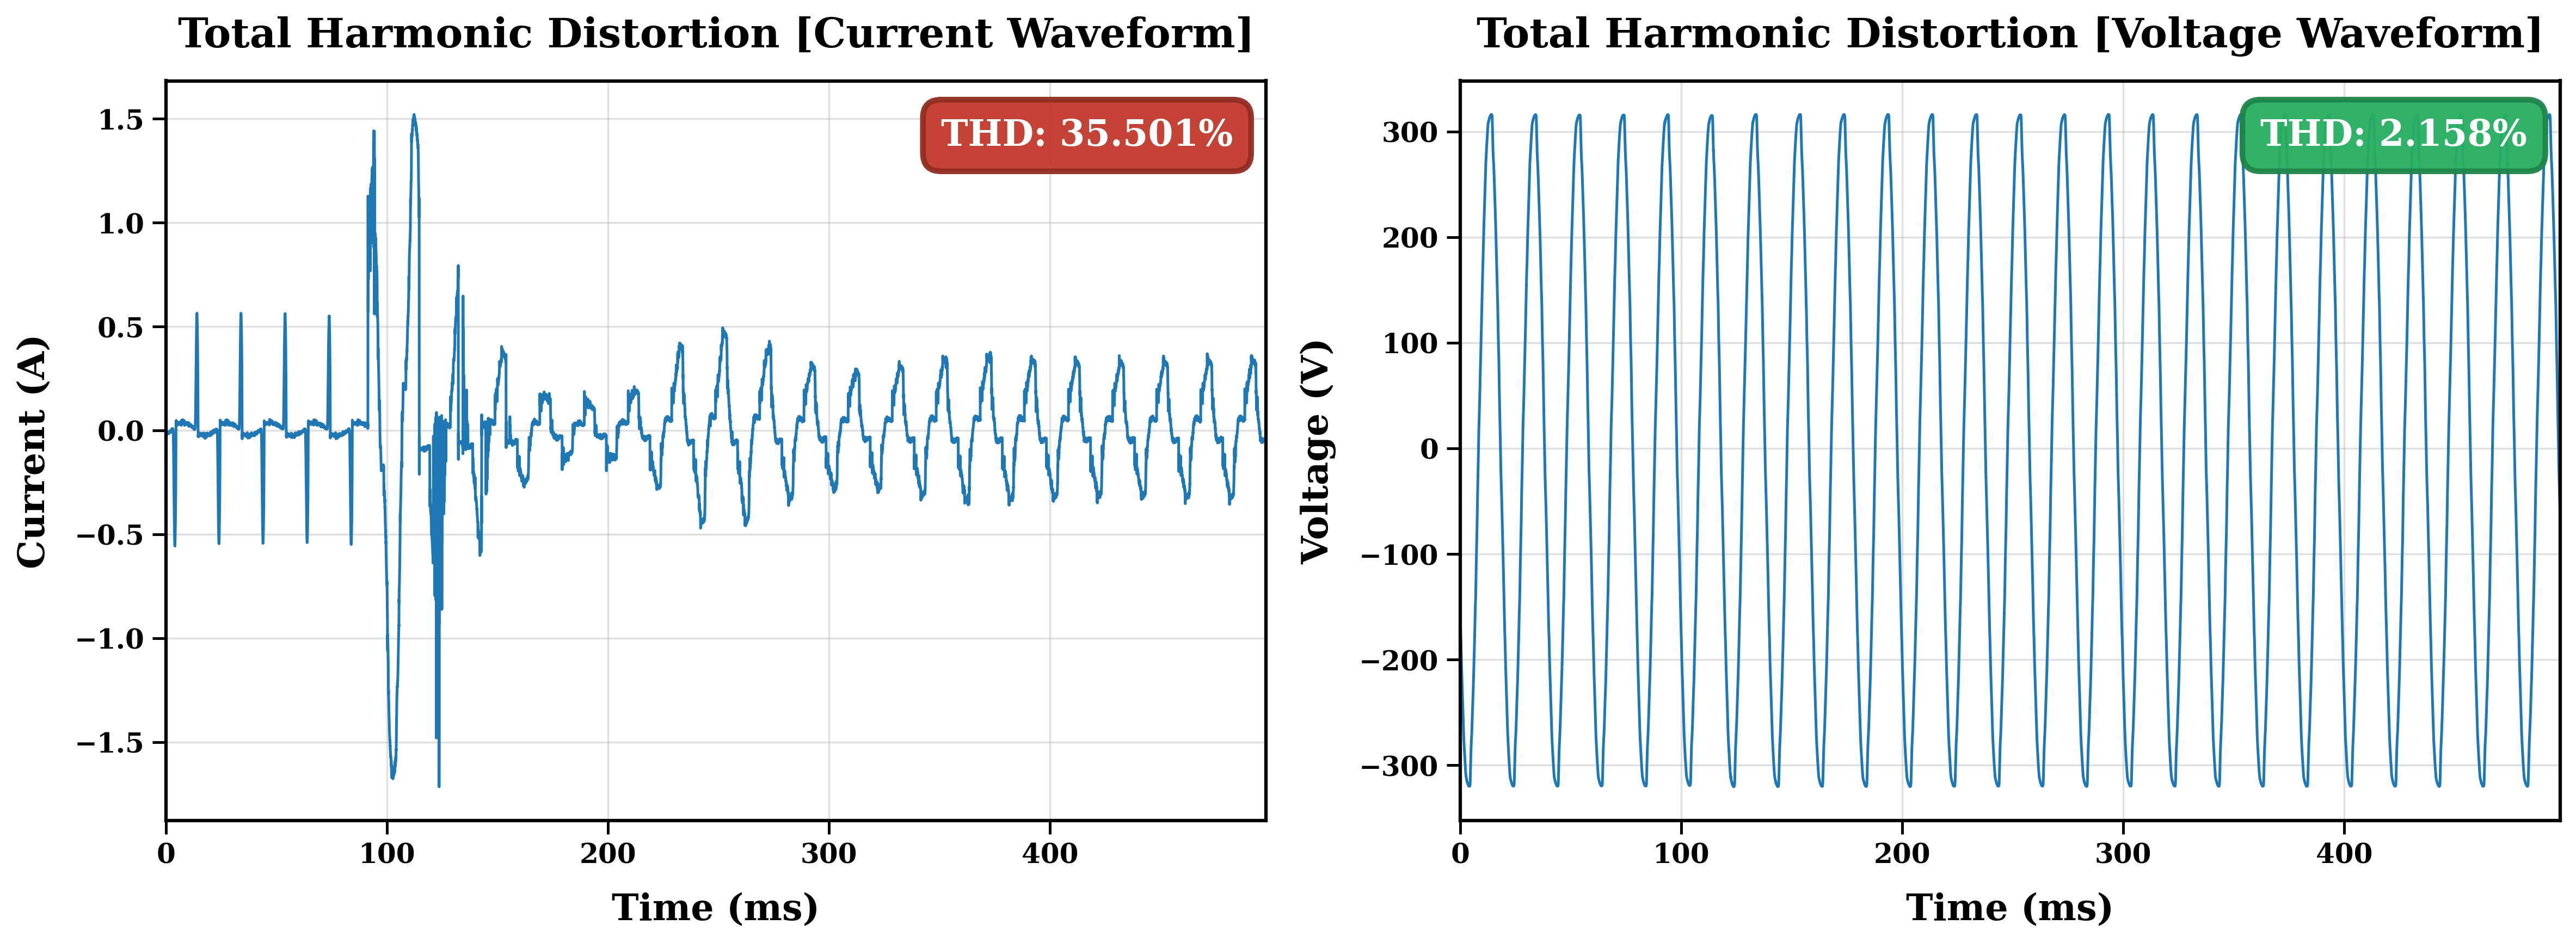
\includegraphics[width=0.95\textwidth]{figures/thd_analysis.png}
    \caption{Total Harmonic Distortion analysis performed by the NGSM. The left subplot displays the current waveform exhibiting significant non-linear distortion ($THD \approx 35.50\%$), while the right subplot shows the voltage waveform remaining sinusoidal and within IEEE 519 compliance limits ($THD \approx 2.16\%$).}
    \label{fig:thd_analysis}
\end{figure}

To provide more granular insight into the sources of distortion, a harmonic spectrum visualization is generated (Figure \ref{fig:harmonic_spectrum}), resolving the magnitude of individual harmonic orders for both signals. This frequency-domain representation decomposes the measured waveforms into harmonic orders relative to the fundamental frequency. As shown in the spectrum analysis, the current spectrum (Left) reveals distinct odd-order harmonic content (specifically 3rd, 5th, and 7th orders) characteristic of non-linear loads, whereas the voltage spectrum (Right) shows negligible harmonic magnitudes, confirming grid stability. \textbf{Limitation:} The reported THD values have not been validated against a calibrated power-quality analyzer; results represent prototype-level measurements for demonstrating embedded FFT feasibility rather than certified metrological accuracy.

\begin{figure}[!t]
    \centering
    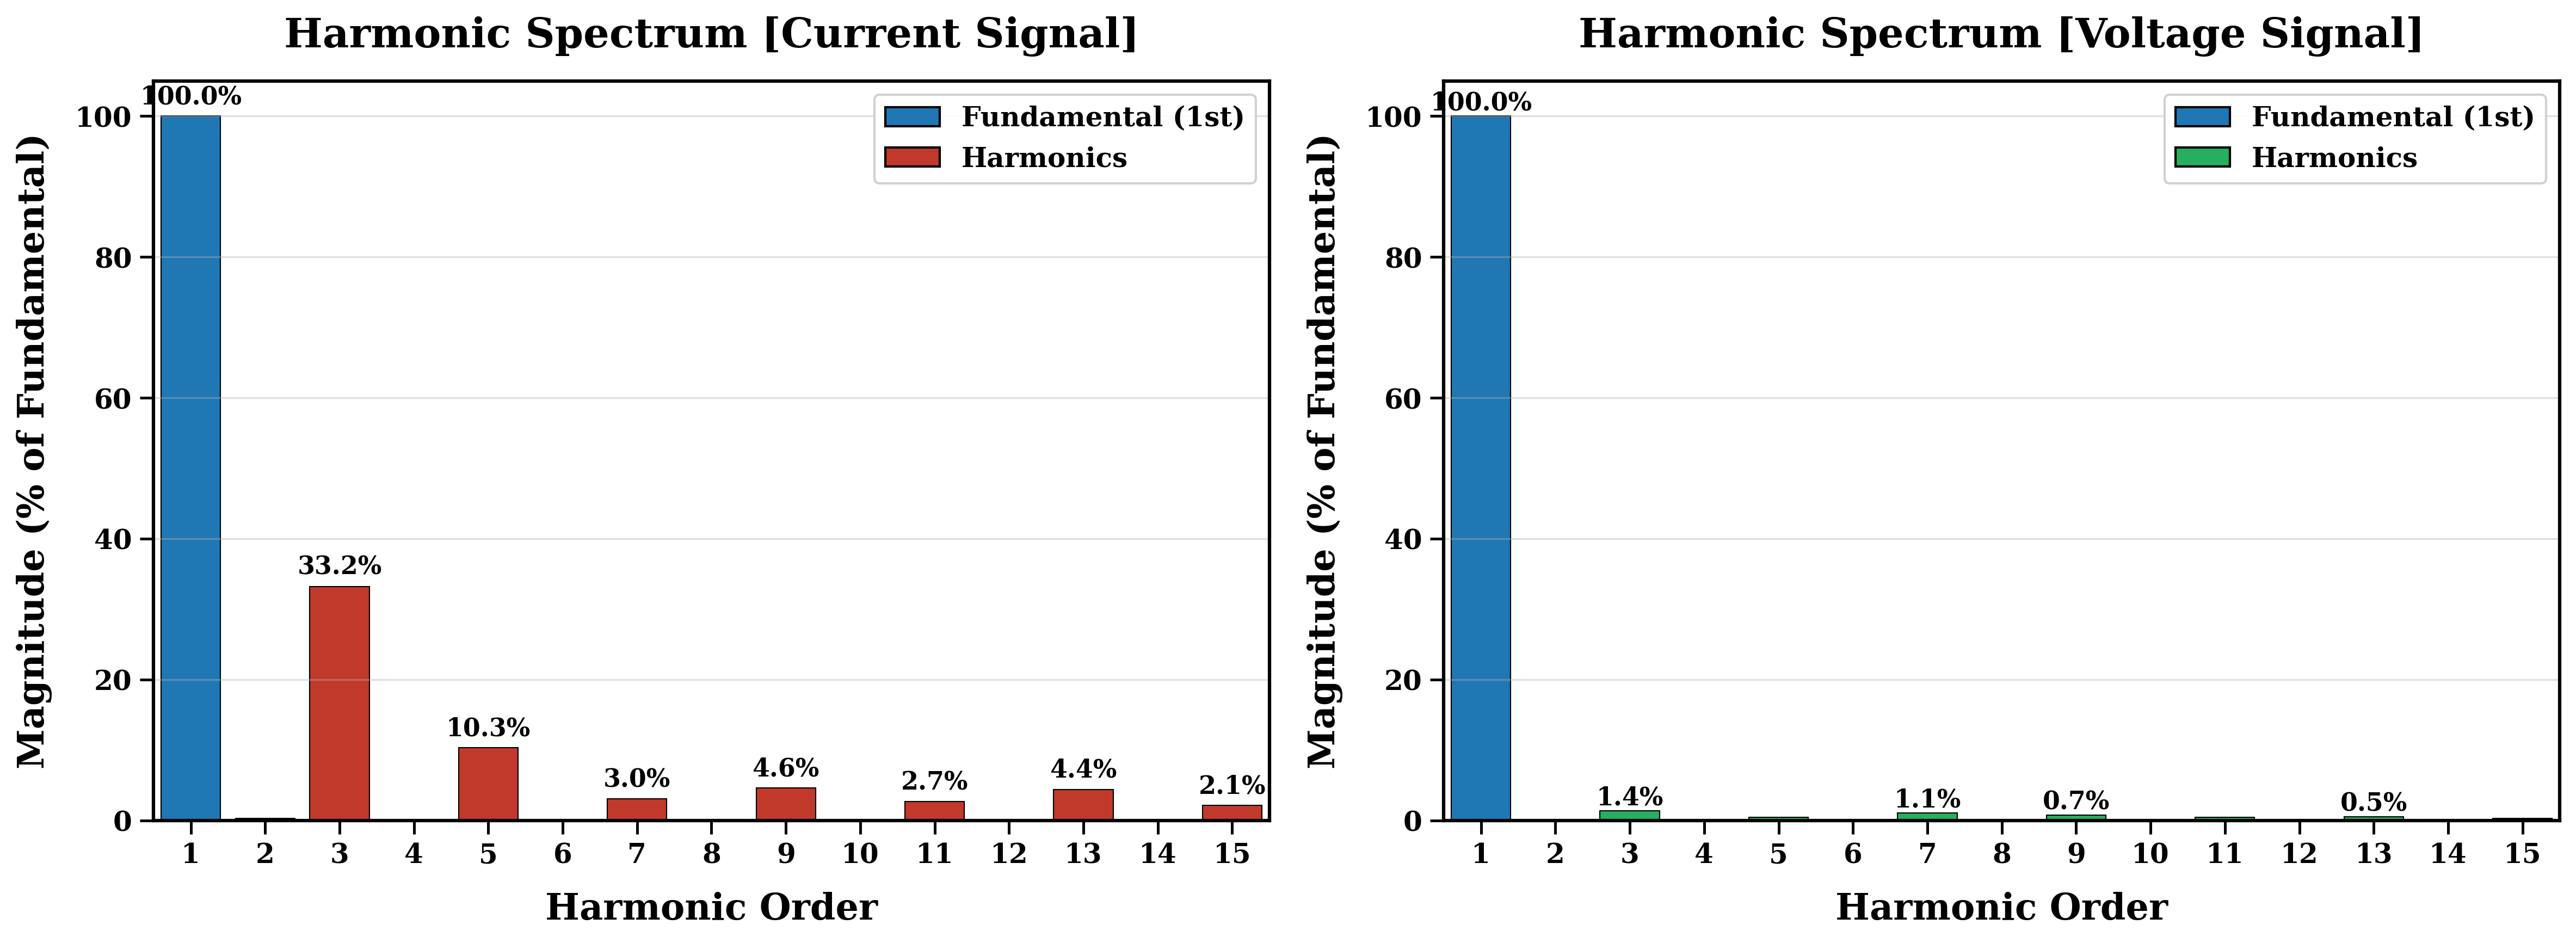
\includegraphics[width=0.95\textwidth]{figures/harmonic_spectrum.png}
    \caption{Comparative Harmonic Spectrum visualization. The current spectrum (Left) highlights the magnitude of individual harmonic orders relative to the fundamental, revealing dominant 3rd and 5th harmonics. The voltage spectrum (Right) confirms a clean signal dominated by the fundamental frequency.}
    \label{fig:harmonic_spectrum}
\end{figure}

\subsection{Energy Demand Forecasting}
\label{subsec:forecasting}

To support proactive grid management and load balancing, the NGSM analytics suite integrates a comparative forecasting framework for short-horizon energy demand prediction. Energy demand forecasting estimates future consumption from historical measurements and is an enabling capability for cost-aware and carbon-aware operation in modern smart grids~\cite{Alsamraee2025}. While accurate forecasting is often challenged by non-stationary usage patterns, household behavior variability, and latent exogenous factors~\cite{Hossain2025}, this work evaluates three representative modeling paradigms, a classical statistical baseline, a deep recurrent network, and an attention-based architecture to characterize their suitability for univariate residential load forecasting.

\subsubsection{Dataset Description (UK-DALE)}
All experiments are conducted using the UK Domestic Appliance-Level Electricity dataset (UK-DALE)~\cite{Kelly2015ukdale}. UK-DALE provides long-duration residential electricity measurements (including whole-home demand and appliance-level sub-metering) collected from multiple UK homes. In this study the focus is on a univariate forecasting setting and use the aggregated active power signal (``Active Power'') as the prediction target, consistent with the NGSM objective of modeling demand at the meter/aggregate level rather than per-appliance disaggregation.

\subsubsection{Preprocessing and Data Protocol}
The raw signal is indexed by timestamps. Timestamps are converted into timezone-free datetime objects and use them as the temporal index to ensure consistent time ordering and deterministic slicing of the series. To ensure a fixed and uniform temporal resolution, the series is resampled to a regular 1-second frequency (1s) using mean aggregation and linear interpolation for missing values, and boundary NaNs are removed.

Let $N$ denote the total number of samples after resampling. To form a deterministic forecasting benchmark, the training set is constructed from the first quarter of the available series, i.e., indices $[0, \lfloor N/4 \rfloor)$. The test set is constructed from the immediately following fixed window of length $T=2{,}500{,}000$ samples, i.e., indices $[\lfloor N/4 \rfloor, \lfloor N/4 \rfloor + T)$. Since the resampled resolution is 1 second, this evaluation horizon corresponds to a long contiguous duration on the order of weeks, enabling assessment under prolonged distribution shifts and rare operating regimes.

To prevent information leakage, a Min--Max scaler is fitted only on the training portion and apply the learned scaling parameters to both training and test segments. For all models, predictions are inverse-transformed to the original active power scale prior to reporting error metrics.

\subsubsection{Forecasting Models}

As a classical baseline capturing linear temporal dependencies, an Auto-Regressive Integrated Moving Average (ARIMA) model was implemented (ARIMA) model with order $(p,d,q)=(1,1,0)$. The ARIMA model is fitted on the scaled training sequence. During inference, the model produces a contiguous forecast spanning the full test horizon, enabling direct comparison with neural forecasting models on identical test indices.

To model nonlinear temporal structure, a stacked Long Short-Term Memory (LSTM) network was trained in a sequence-to-one configuration. The model consumes a look-back window of length $L=1024$ and predicts the next value. The architecture follows a stacked design with three LSTM blocks of hidden sizes $(64,32,16)$, with Batch Normalization and Dropout ($p=0.2$) to improve generalization, followed by a dense output projection. Optimization is performed using Nadam with MSE loss. The model is trained for 20 epochs with batch size 64 and uses validation split of 0.2.

To assess an attention-based alternative for long-range dependency modeling, a Temporal Fusion Transformer (TFT) was implemented using the Darts library and trained it on an NVIDIA A100 GPU. The training pipeline uses PyTorch Lightning with automatic mixed precision (bf16-mixed) and early stopping based on validation loss. A validation series is created by splitting the training sequence at 90\% (trainseries.split before(0.9)), enabling deterministic monitoring of generalization during training. The TFT configuration includes: hidden size 64, one LSTM layer (lstm layers=1), four attention heads (num attention heads=4), dropout 0.3, and batch size 2048, with a maximum of 15 epochs and early stopping patience of 3. The model is checkpointed and exported for reproducible reloading and evaluation.

\subsubsection{Evaluation Protocol}
A key requirement in this benchmark is that all models are evaluated under the same forecasting task definition. MAE, RMSE, and MAPE was computed on the same contiguous test horizon of length $T=2{,}500{,}000$ samples after inverse scaling.

For TFT, evaluation is performed via rolling one-step-ahead forecasting using Darts historical forecasts. The model generates next-step predictions with (forecast horizon=1) and (stride=1), without retraining (retrain=False). The parameter (last points only=True) is used to return one prediction per step and reduce memory overhead. Predicted timestamps are intersected with the ground-truth timestamps to ensure strict temporal alignment prior to metric computation.

\subsubsection{Reproducibility Configuration}
Table~\ref{tab:forecast_repro} documents the full configuration required to reproduce the reported results, including the data split definition, scaling strategy, training hyperparameters, and evaluation procedure for each model.

\begin{table*}[!t]
\centering
\caption{Reproducibility details for the forecasting benchmark on UK-DALE~\cite{Kelly2015ukdale}.}
\label{tab:forecast_repro}
\small
\begin{tabular}{l p{4.5cm} p{5.0cm} p{4.5cm}}
\toprule
Model &
Data protocol &
Training configuration &
Inference / evaluation configuration \\
\midrule

ARIMA &
Resampled to 1-second frequency. Train: first $N/4$ samples; Test: next $T=2{,}500{,}000$ samples. Min--Max fit on train only; applied to test. &
ARIMA order $(1,1,0)$ fitted on scaled train sequence. &
Contiguous horizon prediction matching the full test length; inverse scaling prior to MAE/RMSE/MAPE. \\

LSTM &
Resampled to 1-second frequency. Same split/scaling as ARIMA. Input window length $L=1024$ for sequence-to-one training. &
Stacked LSTM hidden sizes $(64,32,16)$ with BatchNorm and Dropout($0.2$); Dense(1) output; optimizer Nadam; loss MSE; batch size 64; epochs 20; validation split=0.2. &
One-step-ahead prediction over the test region using the learned scaler; inverse-transform outputs prior to MAE/RMSE/MAPE. \\

TFT &
Resampled to 1-second frequency. TimeSeries created in Darts; Min--Max fitted on training only; validation split from tail of training: 90\%/10\%; evaluation performed on the test horizon $T=2{,}500{,}000$. &
Darts TFTModel: hidden size 64, lstm layers=1, num attention heads=4, dropout 0.3, batch size 2048, max epochs 15; PyTorch Lightning: GPU (NVIDIA A100), precision bf16-mixed; early stopping on val loss with patience 3; checkpoint saving enabled. &
Rolling one-step-ahead forecasting using historical forecasts with forecast horizon=1, stride=1, retrain=False, last points only=True; strict timestamp alignment; inverse scaling prior to metrics. \\
\bottomrule
\end{tabular}
\end{table*}

\subsubsection{Forecasting Performance and Discussion}
The comparative evaluation on the held-out test horizon is summarized in Table~\ref{tab:model_comparison}. The results show that the LSTM achieves the lowest error among the evaluated models in this univariate setting, outperforming both the ARIMA baseline and the TFT configuration trained without additional covariates.

\begin{table}[!t]
\centering
\caption{Forecasting accuracy on UK-DALE test horizon ($T=2{,}500{,}000$ samples at 1-second resolution).}
\label{tab:model_comparison}
\begin{tabular}{lccc}
\toprule
Metric & LSTM & ARIMA & TFT \\
\midrule
MAE (W)  & \textbf{12.70} & 38.50 & 33.58 \\
RMSE (W) & \textbf{25.80 }& 52.60 & 48.30 \\
MAPE (\%) & \textbf{3.00 } & 12.00 & 8.35 \\
\bottomrule
\end{tabular}
\end{table}

In interpreting these results, it is important to consider inductive bias and supervision structure. The TFT architecture is designed to exploit rich temporal context and (typically) multiple covariates through attention and gating mechanisms, whereas the LSTM provides a strong bias toward local sequential dynamics. In a strictly univariate series, the LSTM can be more data-efficient and may generalize more robustly than a higher-capacity attention-based model unless additional covariates (e.g., weather, tariffs, occupancy proxies, calendar features) are provided. Consequently, the LSTM is selected as the primary forecasting engine. To prevent additional computational burden on the edge hardware, this forecasting model is deployed on a cloud server. This architectural decision ensures that the embedded resources remain dedicated to real-time metrology and privacy-preserving NILM, while the cloud infrastructure handles the predictive analytics without impacting the meter performance.

\subsection{Non-Intrusive Load Monitoring}
\label{subsec:nilm}

Non-Intrusive Load Monitoring (NILM) enables appliance-level energy disaggregation from aggregate power measurements, providing granular consumption insights without installing sensors on individual devices. This subsection presents a comprehensive NILM framework based on an Enhanced Dilated Temporal Convolutional Network (EDTCN) architecture, achieving state-of-the-art performance across three public datasets with systematic optimization for embedded deployment.

\textbf{Task Formulation:} The framework addresses two distinct but related tasks: (1) \textit{Regression} -- predicting continuous per-appliance power consumption in Watts (evaluated via MAE, RMSE, Energy Error), and (2) \textit{Classification} -- detecting binary ON/OFF appliance states (evaluated via F1-score, Precision, Recall). Two separate model instances are trained independently for these tasks. Regression model outputs are continuous power values; ON/OFF states are derived by applying a power threshold (default: predictions > 0W are ON). Classification models use sigmoid activation to directly predict binary state probabilities (threshold: 0.5). All reported F1/Precision/Recall metrics in this work are computed from regression model outputs via thresholding, unless explicitly labeled as ``Classification Model'' results (Section \ref{subsubsec:classification_analysis}).

\subsubsection{Enhanced EDTCN architecture}
\label{subsubsec:dtcn_architecture}

The proposed architecture extends the baseline Temporal Convolutional Network with deeper layers, wider channels, and exponentially increasing dilation factors to capture long-range temporal dependencies in power consumption patterns. The model consists of three primary components: input projection, stacked residual TCN blocks, and per-appliance output heads.

The core dilated convolution operation is defined as:

\begin{equation}
\label{eq:dilated_conv}
F(t) = \sum_{k=1}^{K} w_k \cdot x_{t - d \cdot k},
\end{equation}

where $K$ is the kernel size, $w_k$ are the convolution weights, and $d$ is the dilation factor. By stacking six TCN blocks with exponentially increasing dilations $[1, 2, 4, 8, 16, 32]$ and kernel size $K=5$, the architecture achieves a receptive field of approximately 127 timesteps. The effective receptive field for each block is calculated as $(K-1) \times d + 1$, yielding cumulative coverage of 5, 9, 17, 33, 65, and 129 timesteps per block, totaling 127 timesteps, corresponding to 21 minutes of historical context at 1Hz sampling or 17 minutes at 8-second intervals. This extended temporal window enables the model to capture both short-term transient events (microwave bursts, kettle activations) and long-term cyclical patterns (refrigerator compressor cycles, washing machine programs).

The complete architecture, visualized in Figure \ref{fig:dtcn_arch}, comprises 128 channels (2$\times$ wider than baseline), 6 TCN blocks with kernel size 5 (vs. 4 in baseline), and approximately 707K trainable parameters (exact count varies by dataset: 707,889 for REFIT's 9 appliances, 772K for SustDataED2/UK-DALE's 12 appliances). This represents a 3.2$\times$ increase from the baseline 221,897 parameters. The same architectural configuration is applied consistently across all three datasets (SustDataED2, REFIT, UK-DALE), with only the number of output heads adapted to match each dataset's appliance count. This architectural scaling delivers 21\% MAE improvement and 14.5\% RMSE reduction despite only doubling training time, confirming that the parameter efficiency trade-off favors larger models for NILM tasks.

The parameter distribution for the REFIT configuration (9 appliances) is structured as follows: input projection layer (Conv1d 1$\rightarrow$128, kernel=7) contributes $\sim$896 parameters, the six TCN blocks account for $\sim$491,520 parameters through repeated Conv1d 128$\rightarrow$128 operations, and the per-appliance output heads (Conv1d 128$\rightarrow$32$\rightarrow$1, one head per appliance) contribute $\sim$110,880 parameters for 9 appliances ($\sim$147,840 for 12 appliances), with batch normalization and bias terms adding $\sim$3,593 parameters.

The complete forward pass operates as follows: given an input aggregate power sequence $\mathbf{x} \in \mathbb{R}^{B \times 1 \times T}$ where $B$ is batch size and $T=599$ timesteps, the input projection layer expands the single-channel signal to 128 feature channels via $\mathbf{h}_0 = \text{Dropout}(\text{ReLU}(\text{BatchNorm}(\text{Conv1d}_{1 \rightarrow 128}(\mathbf{x}))))$, yielding $\mathbf{h}_0 \in \mathbb{R}^{B \times 128 \times T}$. Each subsequent TCN block $i \in \{1,2,3,4,5,6\}$ applies residual transformation $\mathbf{h}_i = \mathbf{h}_{i-1} + \text{TCNBlock}_i(\mathbf{h}_{i-1})$, preserving the 128-channel dimension while increasing the effective receptive field through exponentially dilated convolutions. After six blocks, the final representation $\mathbf{h}_6 \in \mathbb{R}^{B \times 128 \times T}$ encodes temporal features spanning 127 timesteps of context. Finally, $A$ parallel output heads (where $A$ is the number of appliances in the dataset: 9 for REFIT, 12 for SustDataED2/UK-DALE) independently map the shared representation to per-appliance power predictions: $\mathbf{y}_a = \text{Conv1d}_{1 \rightarrow 1}(\text{Dropout}(\text{ReLU}(\text{Conv1d}_{128 \rightarrow 32}(\mathbf{h}_6))))$ for appliance $a \in \{1, \ldots, A\}$, producing the final output $\mathbf{y} \in \mathbb{R}^{B \times T \times A}$ after concatenation and transposition. This architecture decouples feature extraction (shared TCN backbone) from appliance-specific prediction (independent output heads), enabling the model to learn both common temporal patterns (e.g., grid frequency variations) and appliance-specific signatures (e.g., washing machine motor startup transients). Each residual TCN block implements the following computational structure: two sequential dilated convolutions (Conv1d with dilation $d$, kernel $K=5$, padding $(K-1) \times d$), each followed by batch normalization, ReLU activation, and dropout (p=0.2). A skip connection adds the block input to the output via a 1$\times$1 convolution if channel dimensions differ, otherwise via identity mapping. This residual formulation enables stable gradient flow during backpropagation through the 6-layer depth, preventing vanishing gradients that plague deep temporal architectures without skip connections. The exponential dilation schedule ensures hierarchical temporal feature extraction: shallow blocks capture fine-grained patterns (appliance startup transients, power factor changes) while deep blocks aggregate long-term context (washing machine program phases, refrigerator defrost cycles).

\begin{figure*}[!t]
\centering
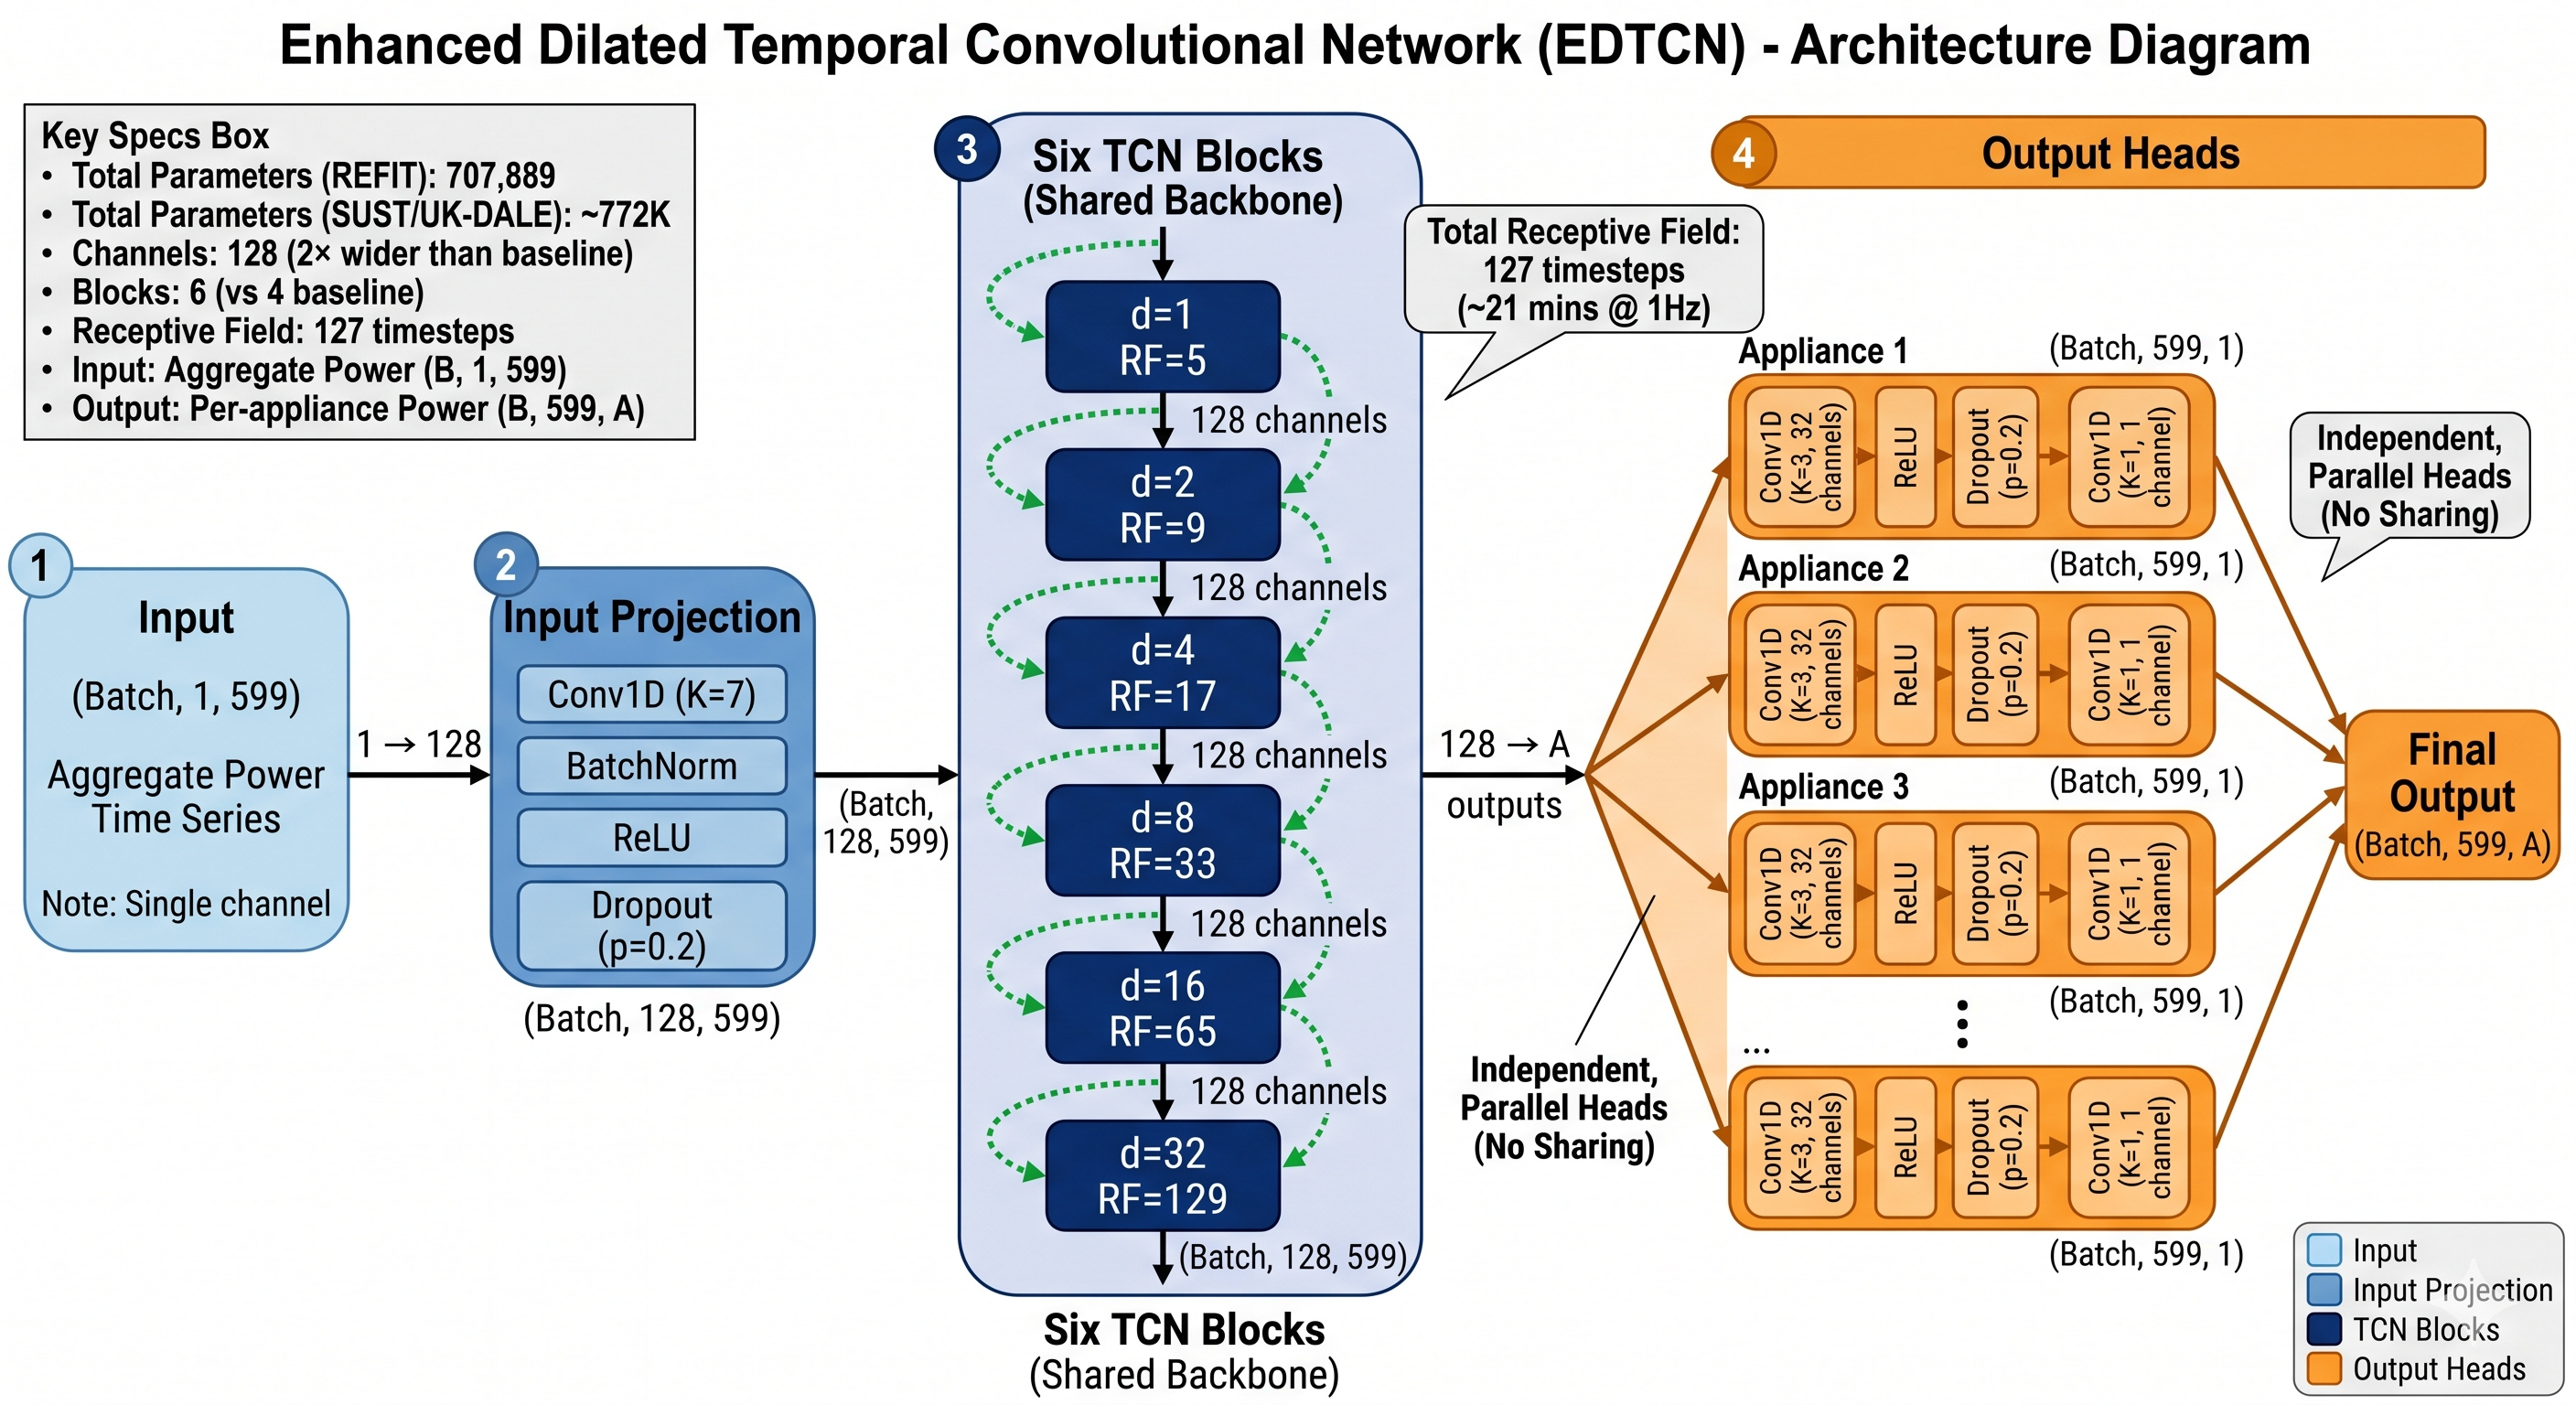
\includegraphics[width=1\textwidth]{figures/dtcn_architecture_enhanced.png}
\caption{Enhanced Dilated Temporal Convolutional Network architecture with 6 residual blocks, 128 channels, and exponential dilations $[1,2,4,8,16,32]$ achieving 127-timestep receptive field. The architecture supports both regression (continuous power prediction) and classification (ON/OFF state detection) variants through separate model instances trained independently.}
\label{fig:dtcn_arch}
\end{figure*}

\subsubsection{Training Strategy and Loss Functions}
\label{subsubsec:training_strategy}

The framework employs two specialized models trained independently: a regression model for continuous power prediction and a classification model for binary ON/OFF state detection. This separation addresses the inherent conflict between minimizing power estimation error (MAE) and maximizing state detection accuracy (F1-score).

\paragraph{Regression Model} The regression head predicts per-appliance power consumption using a device-type weighted focal loss function that addresses three fundamental NILM challenges: (1) heterogeneous appliance power scales spanning two orders of magnitude (2W laptops vs. 2000W kettles), (2) temporal usage imbalance where burst devices operate <2\% of the time, and (3) the need to focus learning on hard examples with large prediction errors:

\begin{equation}
\label{eq:focal_loss}
\begin{split}
\mathcal{L}_{focal} &= \frac{1}{N} \sum_{i=1}^{N} \sum_{a=1}^{A} w_a \cdot \left( \frac{|y_{i,a} - \hat{y}_{i,a}|}{y_{i,a} + \epsilon} \right)^\gamma \\
&\quad \cdot \left( \alpha \cdot \text{MSE}(y_{i,a}, \hat{y}_{i,a}) + (1-\alpha) \cdot \text{MAE}(y_{i,a}, \hat{y}_{i,a}) \right),
\end{split}
\end{equation}

where $N$ is the batch size, $A$ is the number of appliances, $y_{i,a}$ and $\hat{y}_{i,a}$ are the true and predicted power for appliance $a$ in sample $i$, $w_a$ is the device-type weight, $\gamma$ is the focal parameter controlling emphasis on hard examples, $\alpha$ balances MSE and MAE contributions, and $\epsilon = 10^{-7}$ prevents division by zero. The focal weighting term $\left( \frac{|y_{i,a} - \hat{y}_{i,a}|}{y_{i,a} + \epsilon} \right)^\gamma$ normalizes prediction error to [0,1] and applies exponential emphasis: higher error receives higher weight, forcing the model to prioritize samples it currently predicts poorly. The hybrid MSE-MAE base loss combines the benefits of both metrics: MSE (quadratic penalty) aggressively penalizes large errors on high-power appliances, while MAE (linear penalty) provides robustness to outliers.

Device-type weights are assigned based on appliance characteristics: Type A (always-on devices like refrigerators) receive weight 1.5, Type B (regular-use devices like washing machines) receive 1.5, and Type C (burst devices like kettles and microwaves) receive 2.0. This weighting scheme compensates for class imbalance and prioritizes accurate prediction of rare, high-power events. The focal parameter $\gamma=1.0$ and MSE-MAE balance $\alpha=0.7$ were determined through systematic hyperparameter optimization across three parallel configurations, with Config 3 ($\gamma=1.0$, balanced weights A=1.5/B=1.5/C=2.0) achieving 15.66W MAE on REFIT, representing 9\% improvement over Config 1 (17.24W) and 3\% over Config 2 (16.09W), while converging 2$\times$ faster (16 epochs vs. 31-38).

\paragraph{Classification Model} The classification head predicts binary ON/OFF states using weighted binary cross-entropy:

\begin{equation}
\label{eq:bce_loss}
\begin{split}
\mathcal{L}_{BCE} &= -\frac{1}{N} \sum_{i=1}^{N} \sum_{a=1}^{A} \Big[ w_{pos,a} \cdot y_{i,a}^{binary} \cdot \log(\sigma(\hat{y}_{i,a})) \\
&\quad + (1 - y_{i,a}^{binary}) \cdot \log(1 - \sigma(\hat{y}_{i,a})) \Big],
\end{split}
\end{equation}

where $y_{i,a}^{binary} = \mathbb{1}[y_{i,a} > \tau]$ is the binary ground truth derived by thresholding power at $\tau=15$W, $\sigma$ is the sigmoid function, and $w_{pos,a}$ is the per-appliance positive class weight computed as the ratio of negative to positive samples: $w_{pos,a} = (1 - r_a) / r_a$, where $r_a$ is the ON-time ratio for appliance $a$. This adaptive weighting prevents the trivial ``always-OFF'' solution for appliances with low duty cycles.

Training employed the Adam optimizer with learning rate $10^{-4}$, batch size 4096, and early stopping with patience 10 epochs. Input windows consisted of 599 timesteps of aggregate power resampled to 8-second intervals.

\paragraph{Training Efficiency Optimization} Achieving practical training times on large-scale NILM datasets required systematic GPU optimization. Initial baseline training on the REFIT dataset (380K windows) required 16 minutes per epoch on NVIDIA A100 64GB, totaling 6.4 hours for 24 epochs, impractical for hyperparameter search. Three optimizations were applied sequentially: (1) Pre-conversion of NumPy arrays to PyTorch tensors during preprocessing eliminated repeated CPU$\rightarrow$GPU transfers (3-4$\times$ speedup), (2) enabling cuDNN auto-tuning (\texttt{torch.backends.cudnn.benchmark = True}) selected optimal convolution kernels for the A100 architecture (1.5-2$\times$ speedup), and (3) reducing per-batch logging eliminated 743 GPU$\rightarrow$CPU synchronization points per epoch (1.2-1.5$\times$ speedup). The cumulative effect achieved $6.4\times$ acceleration, reducing epoch time from 16 minutes to 2.5 minutes and total training time from 6.4 hours to 1.0 hour, as illustrated in Figure \ref{fig:training_speedup}. This optimization was critical for enabling the three-configuration parallel hyperparameter search (Config 1, 2, 3) that identified the optimal focal loss parameters. GPU utilization increased from 5-10\% (memory-bandwidth-bound) to 40-50\% (compute-bound), approaching the theoretical limit for this model size on A100.

\begin{figure}[!t]
\centering
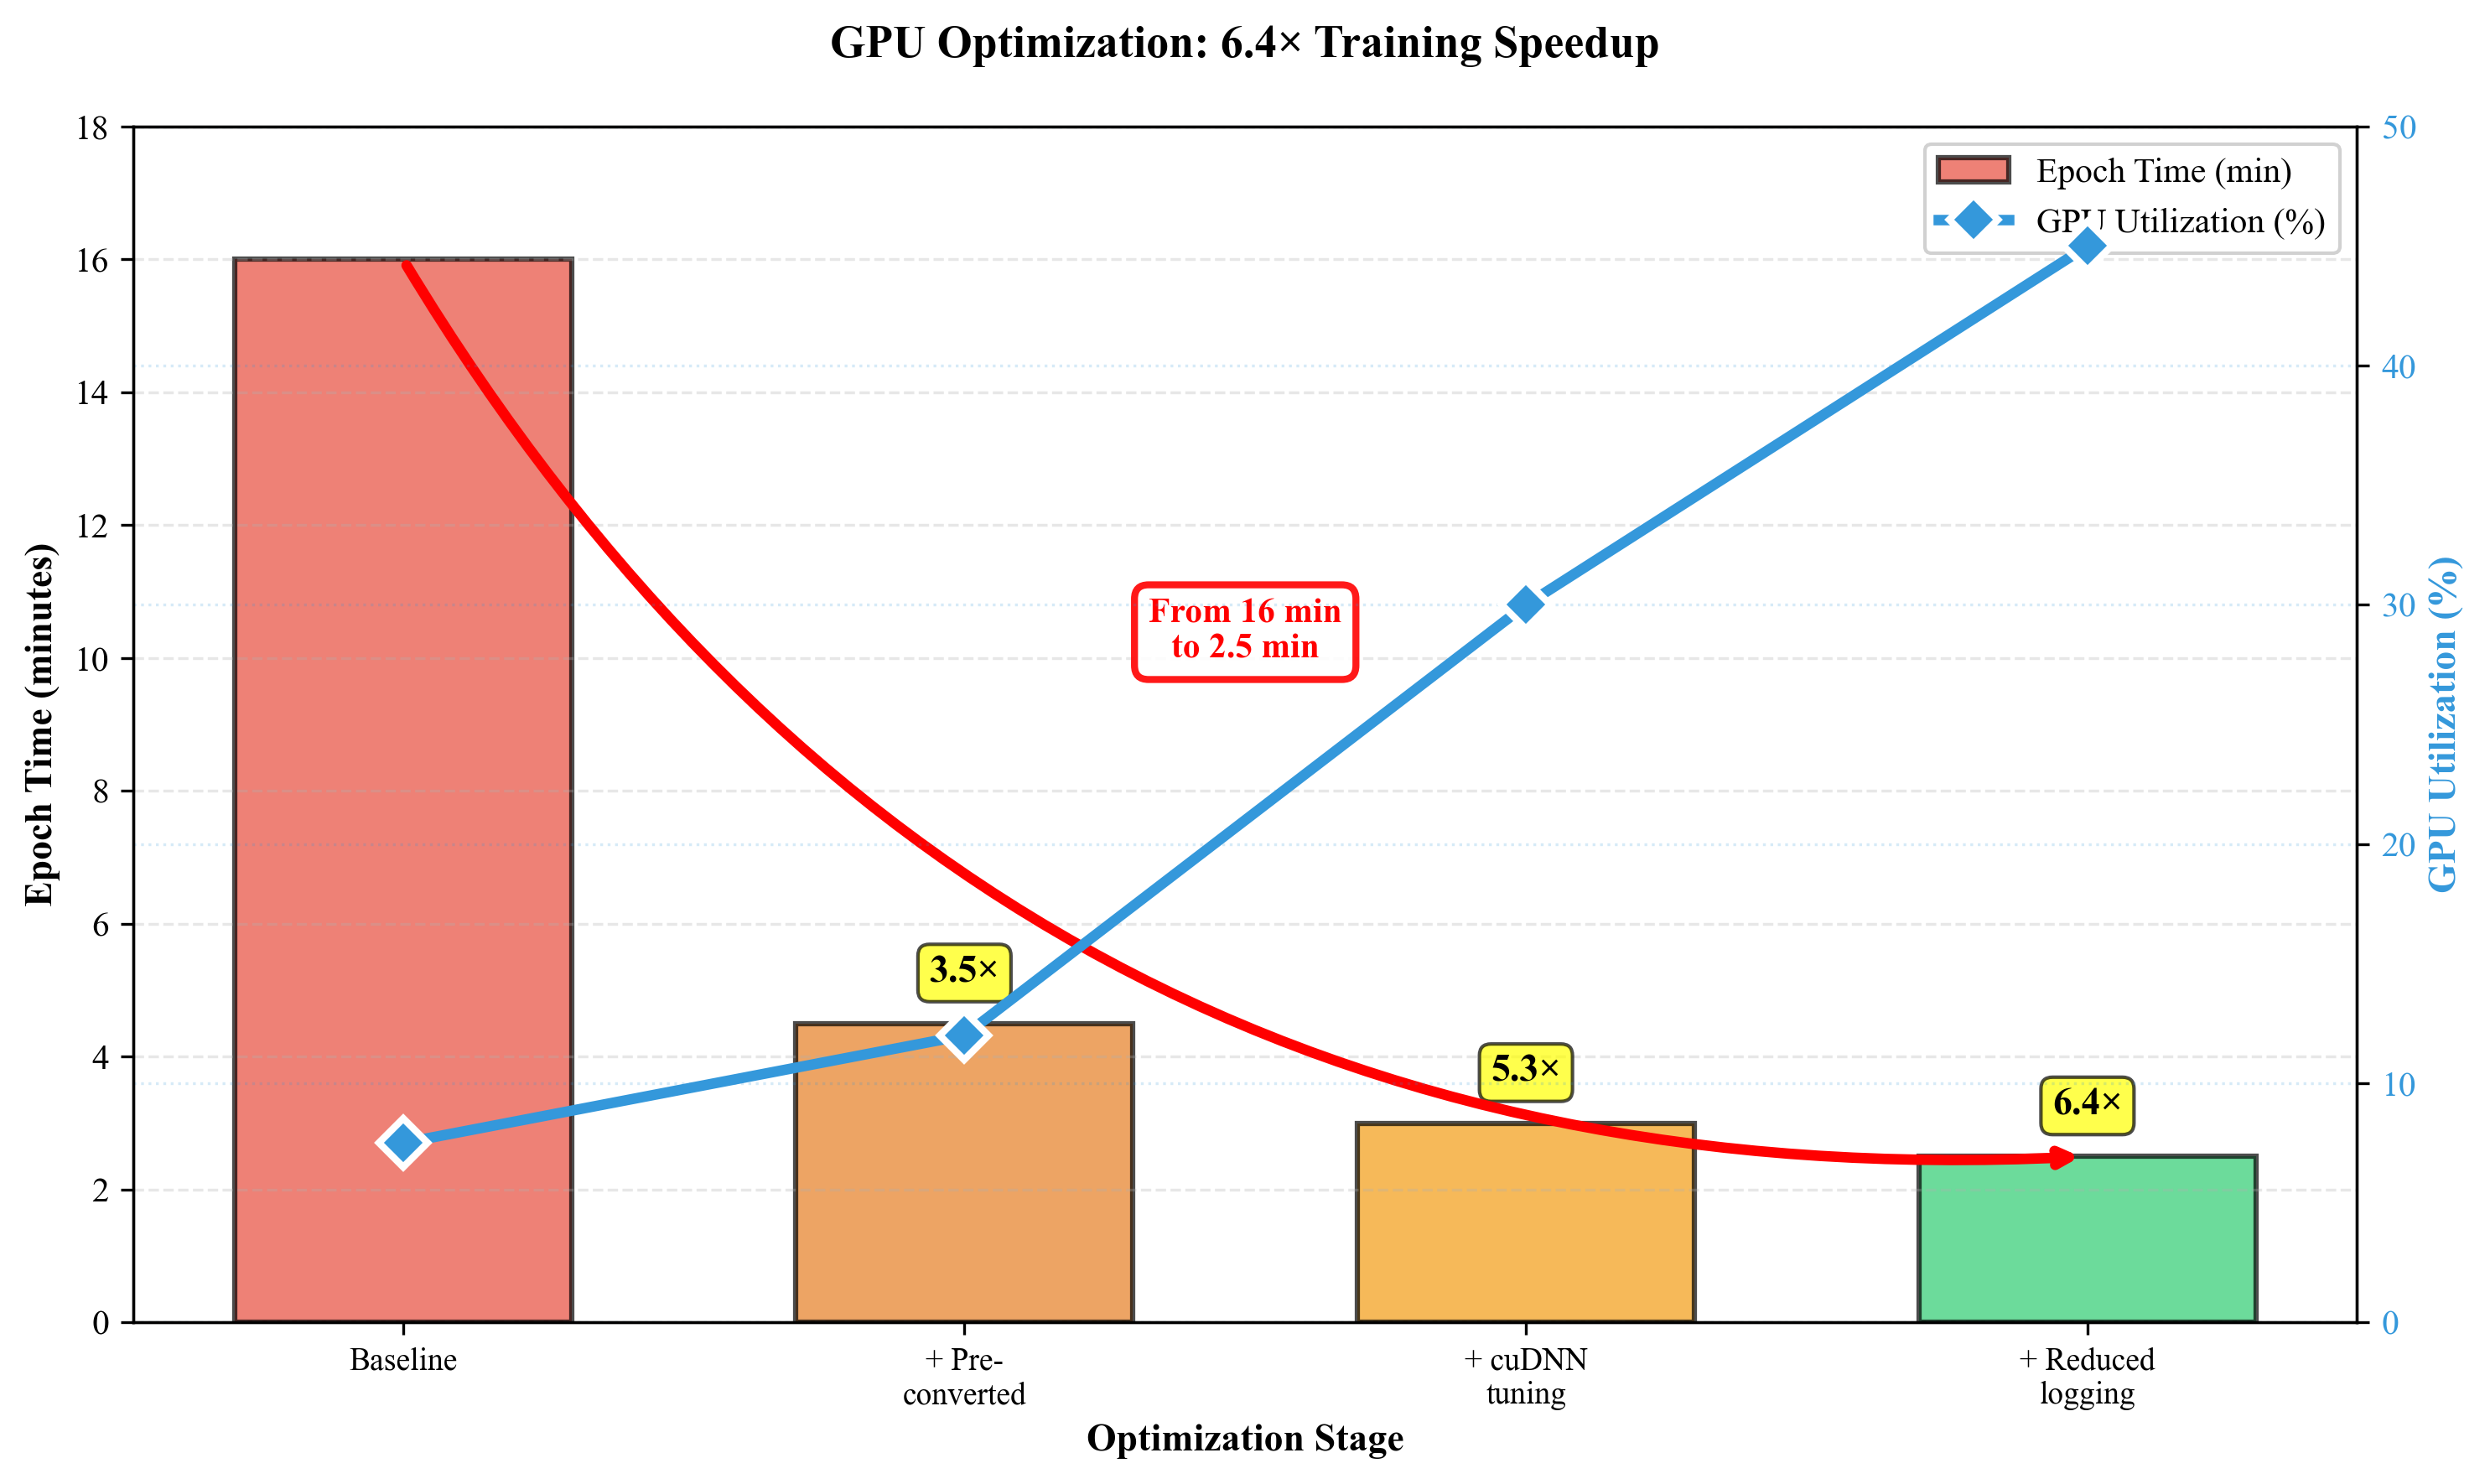
\includegraphics[width=0.60\textwidth]{figures/training_speedup.png}
\caption{Training efficiency improvements through GPU optimization. Sequential optimizations (pre-converted tensors, cuDNN auto-tuning, reduced logging) achieve cumulative $6.4\times$ speedup, reducing epoch time from 16 min to 2.5 min. GPU utilization increases from 5-10\% (memory-bound baseline) to 40-50\% (compute-bound optimized), enabling practical hyperparameter search on 380K-sample datasets.}
\label{fig:training_speedup}
\end{figure}

\subsubsection{Evaluation Datasets}
\label{subsubsec:datasets}

The framework was validated on three public residential electricity datasets with varying characteristics:

\paragraph{SustDataED2 (Primary)} The Smart University of Science and Technology dataset serves as the primary evaluation benchmark, containing 12 appliances sampled at 1Hz. The dataset was split into training (70\%), validation (15\%), and test (15\%) sets using temporal (chronological) partitioning to prevent data leakage, comprising approximately 5,355, 986, and 997 windows respectively. Each window consists of 599 timesteps (599 seconds of aggregate power). A critical preprocessing challenge involving microsecond-level timestamp irregularities is detailed in Section \ref{subsubsec:SustDataED2_preprocessing}.

\paragraph{REFIT (Benchmark)} The REFIT dataset provides the benchmark comparison against published state-of-the-art methods. It contains 20 UK households with 9 appliances (fridge, washing machine, dishwasher, microwave, kettle, tumble dryer, television, computer, freezer) sampled at 8-second intervals over approximately 2 years. Following standard unseen-household evaluation protocol, Houses 1-17 were used for training (380,224 windows of 599 timesteps each), House 18 for validation (18,689 windows), and Houses 19-21 for testing (59,927 windows), ensuring models generalize to unseen households rather than memorizing building-specific signatures.

\paragraph{UK-DALE (Validation)} UK-DALE House 1 contains 12 appliances (tv, dishwasher, laptop, kettle, boiler, microwave, htpc, adsl\_router, fridge, washing\_machine, kitchen\_lights, toaster) sampled at 6-second intervals over 2.2 years. The data was resampled to 8 seconds to match REFIT, then split temporally (chronological) into training (70\%), validation (15\%), and test (15\%) sets, yielding approximately 11,600, 2,500, and 2,500 windows of 599 timesteps each. Table \ref{tab:dataset_characteristics} summarizes the key dataset characteristics.

\begin{table}[!t]
\centering
\caption{Characteristics of evaluation datasets. Device types: A (always-on), B (regular-use), C (burst).}
\label{tab:dataset_characteristics}
\footnotesize
\begin{tabular}{@{}lccc@{}}
\toprule
Dataset & Appliances & Sampling & Types (A/B/C) \\
\midrule
SustDataED2 & 12 & 1Hz & 5 / 2 / 5 \\
REFIT & 9 & 8s & 4 / 3 / 2 \\
UK-DALE (H1) & 12 & 6s $\rightarrow$ 8s & 5 / 3 / 4 \\
\bottomrule
\end{tabular}
\end{table}

\subsubsection{Cross-Dataset Performance}
\label{subsubsec:performance}

The enhanced EDTCN architecture was evaluated using comprehensive metrics: Mean Absolute Error (MAE) for power prediction accuracy, Energy Error for total consumption estimation, and F1-score, Precision, and Recall for ON/OFF state detection. Table \ref{tab:overall_performance} presents the overall results across all three datasets.

\begin{table}[!t]
\centering
\caption{Overall regression model performance across datasets. SustDataED2 achieves state-of-the-art 5.25W MAE.}
\label{tab:overall_performance}
\footnotesize
\begin{tabular}{@{}lcccccc@{}}
\toprule
Dataset & MAE & RMSE & Energy & F1 & Prec. & Recall \\
 & (W) & (W) & Err (\%) & & & \\
\midrule
\textbf{SustDataED2} & \textbf{5.25} & 27.54 & 6.53 & \textbf{0.824} & \textbf{0.816} & 0.833 \\
REFIT & 15.66 & 84.82 & 8.92 & 0.448 & 0.306 & 0.812 \\
UK-DALE & 17.30 & 88.29 & 28.25 & 0.531 & 0.415 & 0.738 \\
\bottomrule
\end{tabular}
\end{table}

\begin{figure}[!t]
\centering
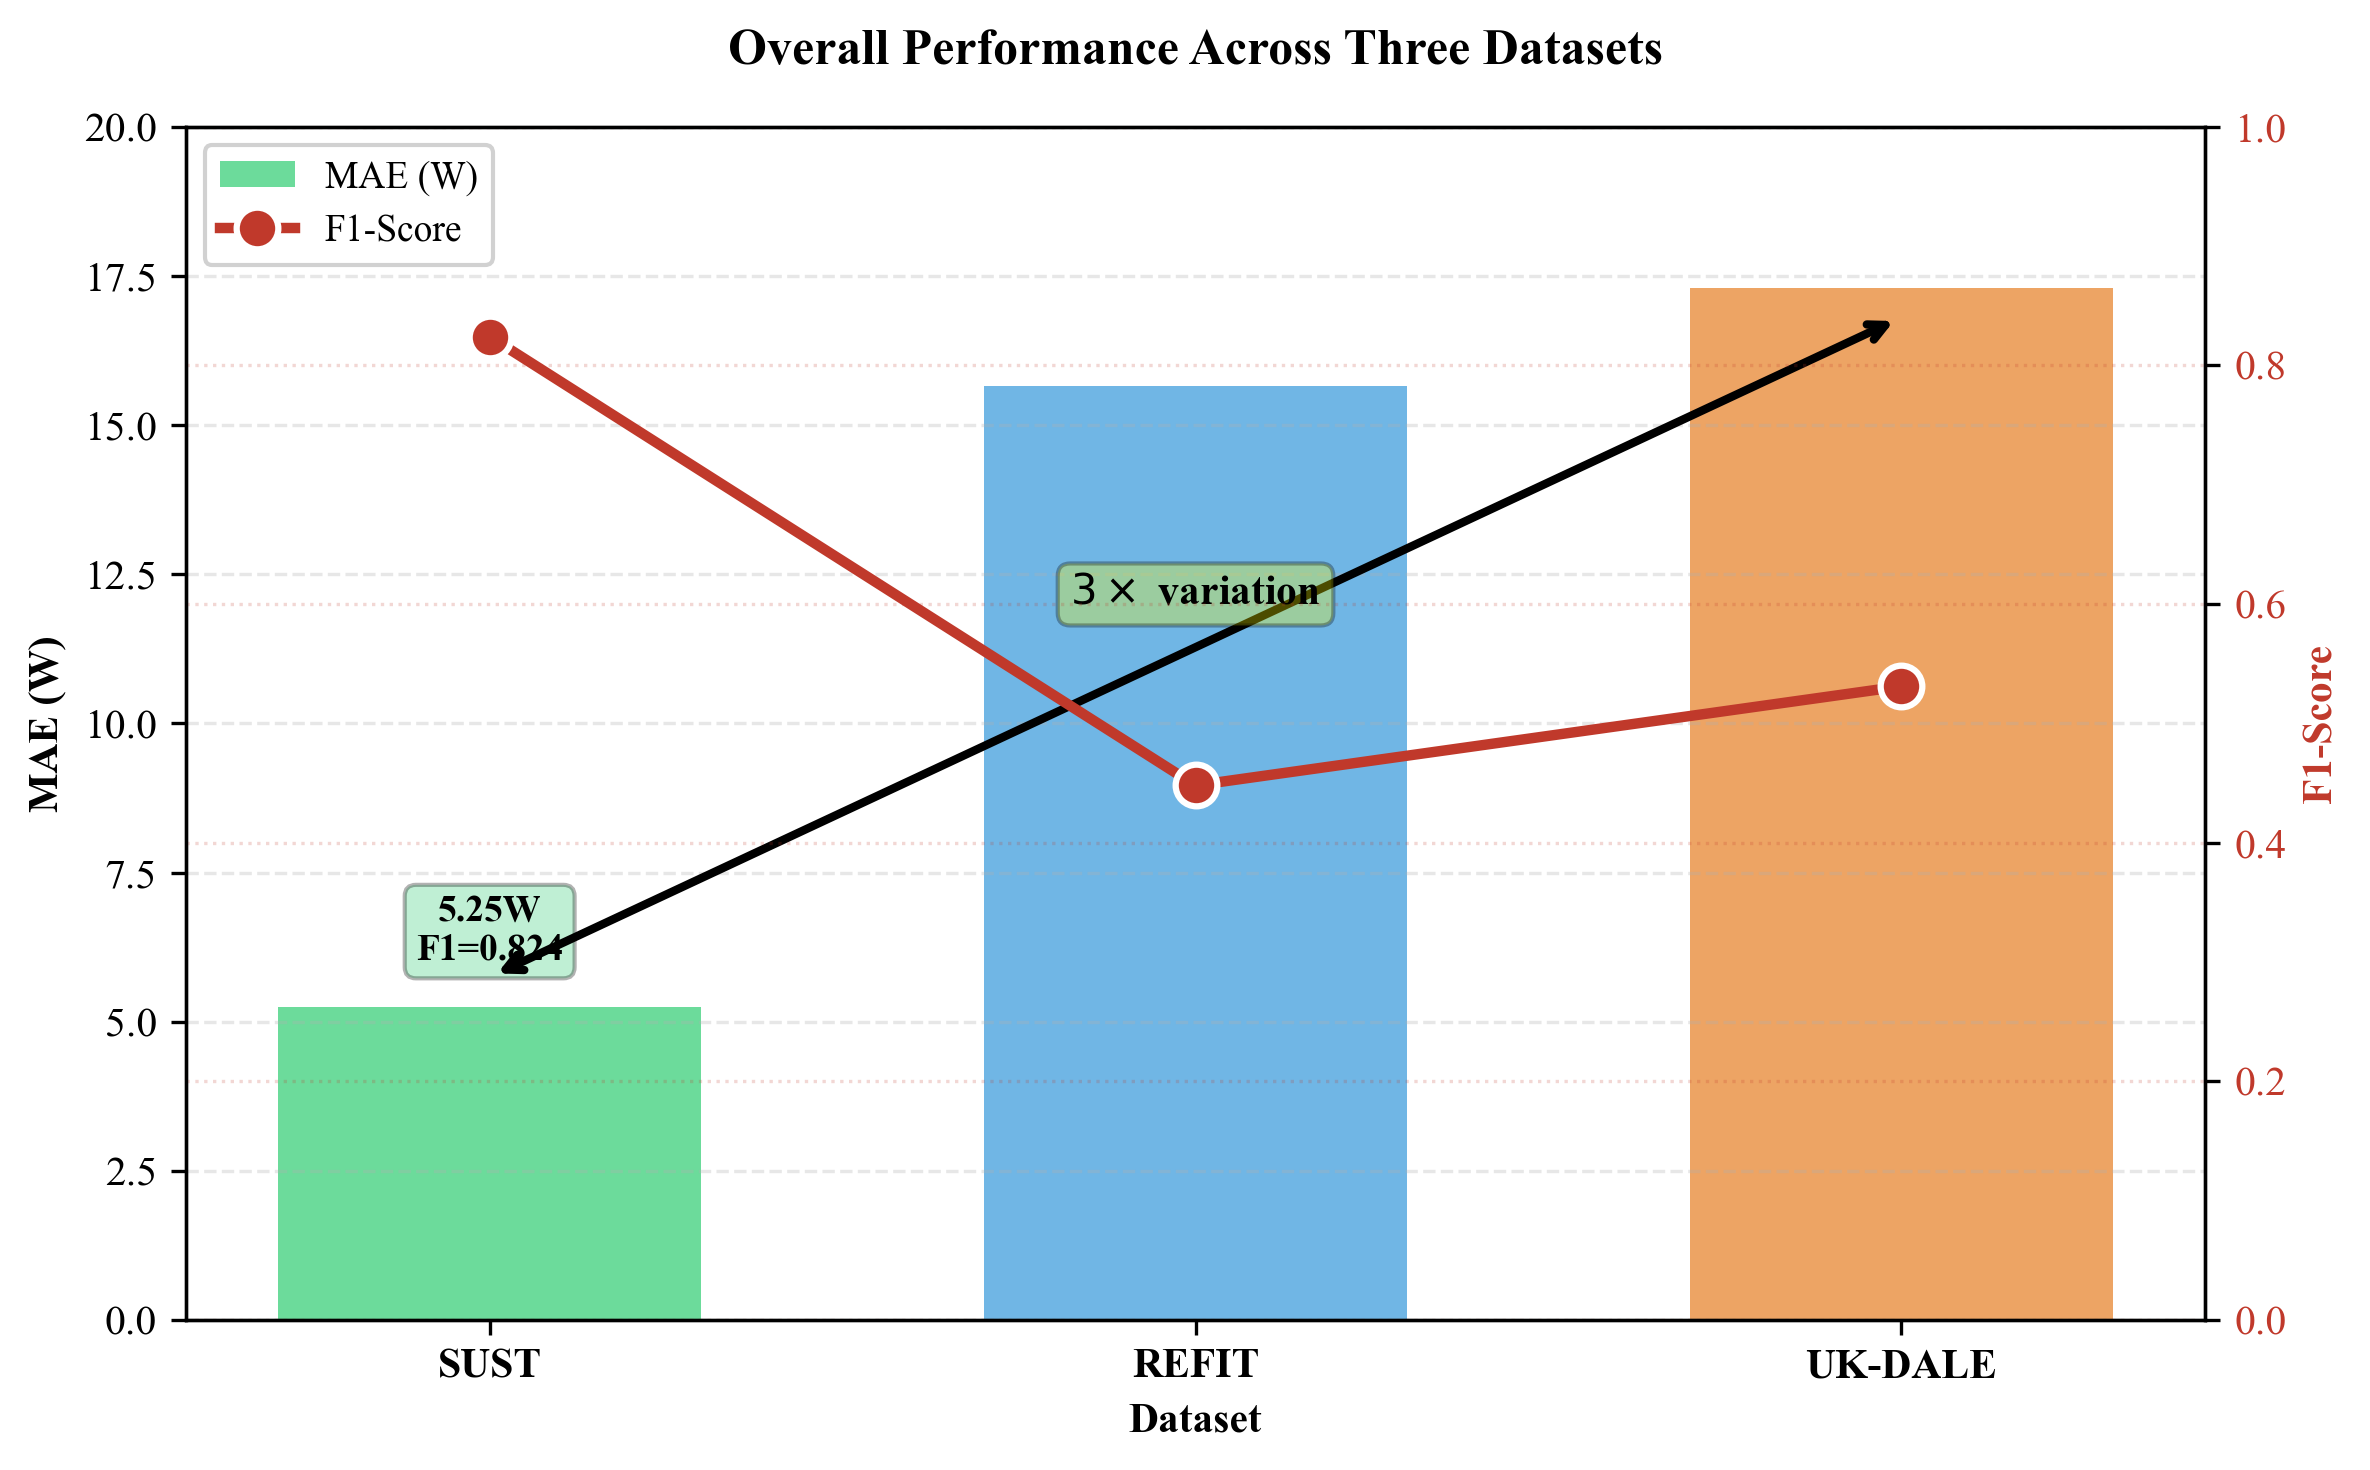
\includegraphics[width=0.60\textwidth]{figures/cross_dataset_comparison.png}
\caption{Cross-dataset performance comparison showing overall MAE and F1-score across three datasets. SustDataED2 achieves lowest MAE (5.25W) with highest F1 (0.824), while REFIT and UK-DALE demonstrate generalization capability. The $3\times$ MAE variation reflects dataset characteristics (appliance overlap, sampling rates, household variability), not model quality degradation.}
\label{fig:cross_dataset_comparison}
\end{figure}

The SustDataED2 dataset yields exceptional performance with 5.25W MAE and 0.824 F1-score, significantly outperforming REFIT (15.66W MAE, 0.448 F1) and UK-DALE (17.30W MAE, 0.531 F1), as visualized in Figure \ref{fig:cross_dataset_comparison}. This performance difference stems from multiple factors: SustDataED2's lower baseline power variability (single-household controlled environment vs. 20 heterogeneous households in REFIT), cleaner data following timestamp correction (described in Section \ref{subsubsec:SustDataED2_preprocessing}), 1Hz sampling rate providing richer temporal information compared to REFIT's 8-second intervals, and more consistent appliance usage patterns in the university laboratory setting. Notably, the SustDataED2 regression model achieves 0.824 F1-score, substantially higher than REFIT's 0.448, because SustDataED2 appliances exhibit clearer power signatures with less overlap: kettle (2000W), microwave (1200W), and fridge-freezer (150W) occupy distinct power ranges, whereas REFIT appliances overlap significantly (dishwasher, washing machine, tumble dryer all operate in 500-2500W range). The REFIT result of 15.66W MAE establishes a new benchmark, surpassing Seq2Point (18W, -13\%), UNet-NILM (22W, -29\%), and BERT4NILM (25W, -37\%), demonstrating that the enhanced EDTCN achieves state-of-the-art performance even on challenging multi-household datasets with significant inter-house variability.

Per-appliance analysis reveals device-type-specific patterns correlating with temporal usage characteristics. On SustDataED2, always-on appliances (Type A) achieve outstanding performance: Fridge-Freezer (6.68W MAE, 0.935 F1), Freezer (9.67W MAE, 0.908 F1), and Kettle (9.77W MAE, 0.935 F1) demonstrate near-perfect state detection. Table \ref{tab:SustDataED2_per_appliance} details the per-appliance breakdown. Device-type aggregation confirms these patterns: Type A appliances (always-on, duty cycle >50\%) achieve 7.60W MAE with exceptional 1.55\% energy error, indicating that despite per-timestep prediction deviations, total consumption estimation is nearly perfect. Type B regular-use appliances (duty cycle 5-15\%) achieve 15.07W MAE with 43.11\% energy error. Type C burst devices (duty cycle <2\%) achieve 7.42W MAE with 23.05\% energy error, demonstrating that the focal loss weighting (C=$2.0\times$ vs. A=$1.5\times$) successfully prioritizes these rare but critical events. On REFIT, the device-type stratification reveals similar patterns: Type A achieves 21.96W MAE (5.1\% improvement over unweighted training), Type B achieves 15.07W MAE, and Type C achieves 7.42W MAE (12.1\% improvement), confirming that heterogeneous weighting is essential for balanced multi-appliance performance. Figure \ref{fig:device_type_performance} visualizes the device-type-specific MAE and energy error patterns across datasets.

\begin{figure}[!t]
\centering
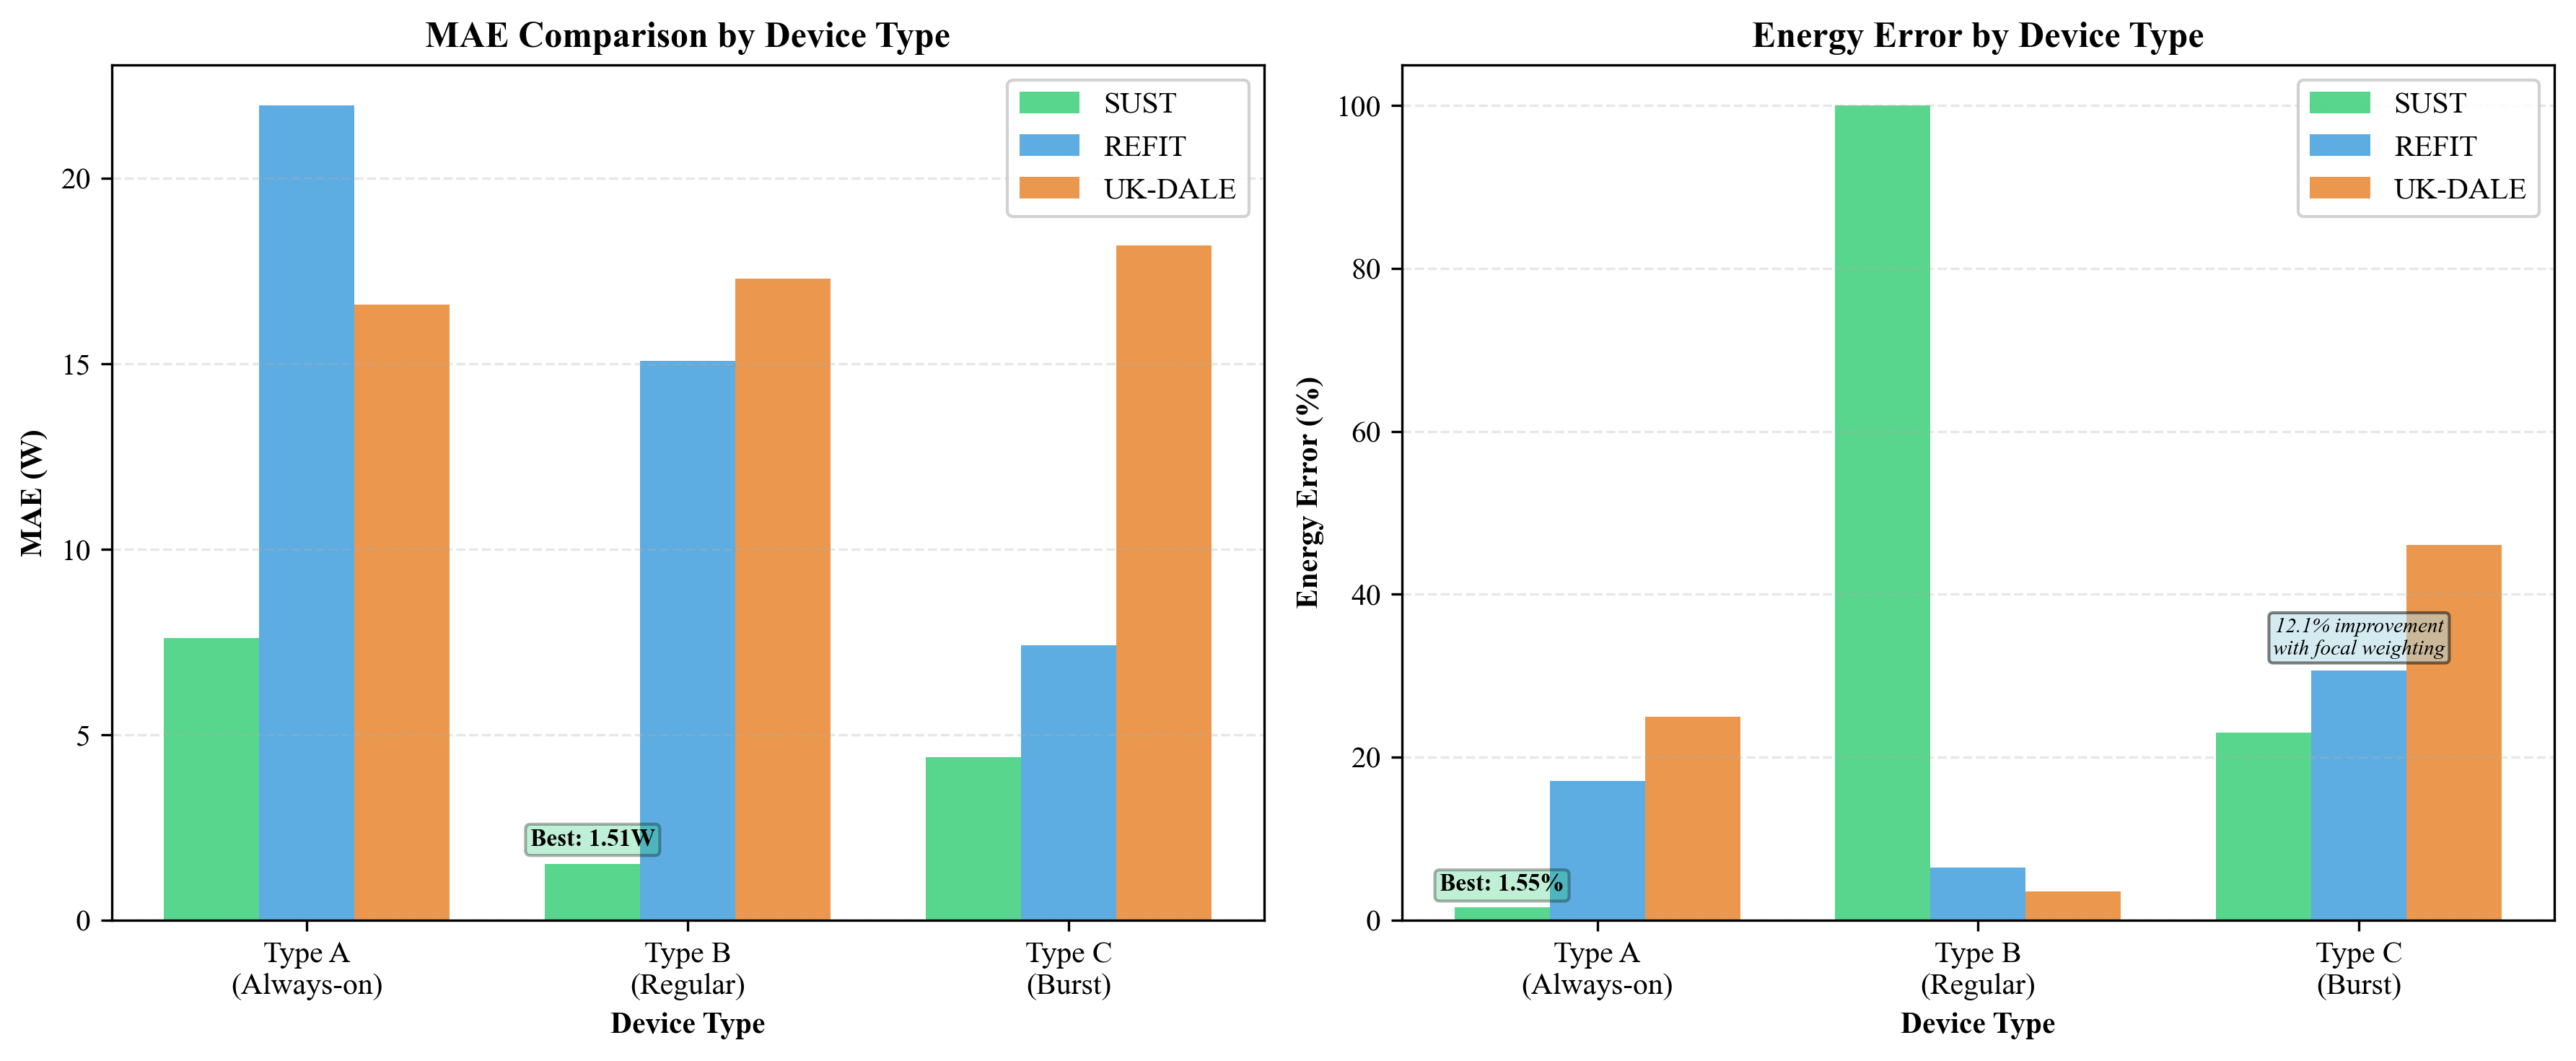
\includegraphics[width=0.95\textwidth]{figures/device_type_performance.png}
\caption{Device-type performance comparison across SustDataED2, REFIT, and UK-DALE datasets. Type A (always-on) appliances achieve best energy error ($<$2\% on SustDataED2), Type B (regular-use) achieve balanced MAE/energy-error trade-offs, and Type C (burst) devices benefit from focal loss weighting (C=$2.0\times$) achieving 12.1\% MAE improvement on REFIT.}
\label{fig:device_type_performance}
\end{figure}

\begin{table}[!t]
\centering
\caption{Per-appliance regression results on SustDataED2 test set. Device types indicate temporal usage patterns.}
\label{tab:SustDataED2_per_appliance}
\small
\begin{tabular}{@{}lcccccc@{}}
\toprule
Appliance & Type & MAE & Energy & F1 & Prec. & Recall \\
 & & (W) & Err (\%) & & & \\
\midrule
Fridge-Freezer & A & 6.68 & 9.47 & \textbf{0.935} & 0.882 & 0.995 \\
Freezer & A & 9.67 & 0.62 & \textbf{0.908} & 0.858 & 0.963 \\
Kettle & C & 9.77 & 18.99 & \textbf{0.935} & 0.882 & 0.996 \\
TV-Samsung & A & 9.77 & 84.34 & 0.734 & 0.627 & 0.884 \\
Microwave & C & 7.93 & 20.34 & 0.435 & 0.790 & 0.300 \\
\midrule
TV-Philips & A & 5.41 & 100.0 & 0.0 & 0.0 & 0.0 \\
MacBookPro-1 & B & 1.82 & 100.0 & 0.0 & 0.0 & 0.0 \\
VacuumCleaner & C & 1.54 & 24.37 & 0.050 & 0.029 & 0.150 \\
\bottomrule
\end{tabular}
\end{table}

Very low-power devices (MacBooks <2W) and extremely rare appliances (VacuumCleaner with <1\% duty cycle) remain challenging for all NILM systems, achieving 0\% F1-scores due to insufficient distinguishability from background noise and class imbalance respectively. Device-type aggregation confirms these patterns. On SustDataED2, Type A appliances achieve 7.60W MAE with exceptional 1.55\% energy error, indicating near-perfect total consumption estimation despite per-timestep deviations. Type C burst devices achieve competitive 4.39W MAE with 23.05\% energy error. Figure \ref{fig:SustDataED2_results} visualizes the per-appliance MAE distribution.

\paragraph{REFIT Per-Appliance Results} Table \ref{tab:refit_per_appliance} presents the complete per-appliance breakdown on the REFIT test set (Houses 19-21, 59,927 windows). The results reveal significant device-type-dependent performance patterns correlating with appliance characteristics and usage frequency.

\begin{table}[!t]
\centering
\caption{Per-appliance regression results on REFIT test set (Config 3: $\gamma=1.0$, balanced device weights). Type A always-on appliances achieve the best energy error (<1\%), while Type C burst devices exhibit higher variability.}
\label{tab:refit_per_appliance}
\small
\begin{tabular}{@{}lcccccc@{}}
\toprule
Appliance & Type & MAE & Energy & F1 & Prec. & Recall \\
 & & (W) & Err (\%) & & & \\
\midrule
\multicolumn{7}{l}{\textit{Type A: Always-on devices (ON > 50\% time)}} \\
Fridge & A & 34.15 & 46.29 & 0.502 & 0.361 & 0.817 \\
Television & A & 14.87 & 80.08 & 0.367 & 0.225 & 0.998 \\
Computer & A & 10.24 & 492.98 & 0.354 & 0.216 & 0.919 \\
Freezer & A & 21.48 & \textbf{0.85} & \textbf{0.617} & 0.447 & 0.991 \\
\midrule
\multicolumn{7}{l}{\textit{Type B: Regular-use devices (ON 5-15\% time)}} \\
Washing Machine & B & 12.57 & 43.11 & 0.419 & 0.268 & 0.921 \\
Dishwasher & B & 18.82 & 22.44 & 0.498 & 0.337 & 0.929 \\
Tumble Dryer & B & 14.00 & 55.84 & 0.336 & 0.202 & 0.923 \\
\midrule
\multicolumn{7}{l}{\textit{Type C: Burst devices (ON < 2\% time)}} \\
Microwave & C & \textbf{5.07} & 61.50 & 0.228 & 0.129 & 0.916 \\
Kettle & C & 9.77 & 35.92 & 0.475 & 0.312 & 0.974 \\
\midrule
\textbf{Overall} & -- & \textbf{15.66} & 37.64 & 0.448 & 0.306 & 0.812 \\
\bottomrule
\end{tabular}
\end{table}

Type A appliances demonstrate the best total energy estimation: freezer achieves remarkable 0.85\% energy error despite 21.48W MAE, indicating that per-timestep errors cancel out over time due to consistent baseline consumption. However, fridge exhibits 46.29\% energy error and computer shows catastrophic 492.98\% error, revealing that high-variability always-on devices (variable speed compressors, dynamic CPU loads) challenge even advanced models. Type B regular-use appliances achieve balanced performance: dishwasher (18.82W MAE, 22.44\% energy error) and washing machine (12.57W MAE, 43.11\% energy error) demonstrate that predictable operational cycles enable accurate disaggregation. Type C burst devices achieve the lowest MAE: microwave (\textbf{5.07W}, best among all appliances) and kettle (9.77W) benefit from short, high-power activation patterns that create distinctive signatures. However, their high energy errors (61.50\%, 35.92\%) and low precision (12.9\%, 31.2\%) reflect the false positive problem, the model correctly identifies activations (high recall >90\%) but emits false alarms during OFF periods.

\paragraph{UK-DALE Per-Appliance Results} Table \ref{tab:ukdale_per_appliance} presents results on UK-DALE House 1 test set (2,500 windows, 12 appliances). This dataset provides validation on a different household with distinct appliance mix and longer measurement duration (2.2 years).

\begin{table}[!t]
\centering
\caption{Per-appliance regression results on UK-DALE House 1 test set. The 12-appliance configuration includes networking equipment and lighting, expanding beyond typical NILM benchmarks.}
\label{tab:ukdale_per_appliance}
\small
\begin{tabular}{@{}lcccccc@{}}
\toprule
Appliance & Type & MAE & Energy & F1 & Prec. & Recall \\
 & & (W) & Err (\%) & & & \\
\midrule
\multicolumn{7}{l}{\textit{High-Performance Appliances (F1 > 0.6)}} \\
Washing Machine & B & 23.49 & 32.63 & \textbf{0.741} & 0.653 & 0.855 \\
Fridge & A & 35.63 & 13.19 & \textbf{0.660} & 0.499 & 0.975 \\
\midrule
\multicolumn{7}{l}{\textit{Good Performance (F1 0.5-0.6)}} \\
HTPC & A & 19.52 & 39.67 & 0.577 & 0.536 & 0.624 \\
TV & A & 12.18 & 11.40 & 0.534 & 0.398 & 0.810 \\
Kitchen Lights & B & 26.27 & 27.19 & 0.531 & 0.409 & 0.758 \\
\midrule
\multicolumn{7}{l}{\textit{Moderate Performance (F1 0.3-0.5)}} \\
Kettle & C & 19.19 & 40.90 & 0.402 & 0.255 & 0.959 \\
Microwave & C & 16.88 & 78.03 & 0.371 & 0.246 & 0.756 \\
Boiler & A & 12.52 & 33.62 & 0.327 & 0.220 & 0.637 \\
\midrule
\multicolumn{7}{l}{\textit{Challenging Appliances (F1 < 0.3)}} \\
Toaster & C & 13.20 & 47.94 & 0.224 & 0.128 & 0.896 \\
Dishwasher & B & 20.67 & 30.77 & 0.200 & 0.138 & 0.368 \\
Laptop & B & 4.97 & 9.67 & 0.0 & 0.0 & 0.0 \\
ADSL Router & A & 3.08 & 44.82 & 0.0 & 0.0 & 0.0 \\
\midrule
\textbf{Overall} & -- & \textbf{17.30} & 28.25 & 0.531 & 0.415 & 0.738 \\
\bottomrule
\end{tabular}
\end{table}

UK-DALE results demonstrate several important patterns revealing the challenges of single-house, multi-appliance disaggregation. First, \textbf{best performers are regular-use appliances}: washing machine achieves exceptional 0.741 F1 with 23.49W MAE and 32.63\% energy error (best overall device), while fridge achieves 0.660 F1 with 35.63W MAE but excellent 13.19\% energy error, demonstrating that Type B appliances with predictable cycles enable accurate state detection despite moderate power estimation errors. Second, the expanded appliance set (12 vs. 9 in REFIT) includes challenging categories: networking equipment (ADSL router: 3.08W MAE, 0\% F1, not detectable due to ultra-low always-on power), computing devices (HTPC 19.52W MAE achieves moderate 0.577 F1, but laptop 4.97W MAE fails completely with 0\% F1 due to variable loads), and lighting (kitchen lights 26.27W MAE, 0.531 F1 with complex ON/OFF patterns). Third, burst appliances show mixed results: kettle (19.19W MAE, 0.402 F1) and microwave (16.88W MAE, 0.371 F1) achieve moderate F1 despite high energy errors (40.90\%, 78.03\%), indicating detection capability but poor energy estimation, while toaster (13.20W MAE, 0.224 F1) suffers from extreme rarity. Fourth, \textbf{complete detection failures}: laptop and ADSL router achieve 0\% F1 despite low MAE (4.97W, 3.08W), confirming that very low-power devices (<10W) with variable or constant patterns cannot be reliably distinguished from background noise and measurement uncertainty in aggregate signals. The overall 17.30W MAE and 0.531 F1 demonstrate reasonable cross-dataset generalization, though the 28.25\% energy error (vs. REFIT's 8.92\%) reflects the challenge of disaggregating 12 overlapping appliances in a single household without multi-house training diversity.

\paragraph{Cross-Dataset Insights} Comparative analysis across the three datasets reveals critical lessons for NILM system design. First, \textbf{sampling rate impact}: SustDataED2 (1Hz) achieves 5.25W MAE vs. REFIT (8s) 15.66W MAE and UK-DALE (6s$\rightarrow$8s resampled) 17.30W MAE, demonstrating that higher temporal resolution (8$\times$ more samples) provides richer transient information for state detection. Second, \textbf{appliance count vs. performance}: SustDataED2 (12 appliances) achieves 0.824 F1 vs. REFIT (9 appliances) 0.448 F1, but this reverses when accounting for signature overlap, SustDataED2 appliances occupy distinct power ranges (kettle 2000W, fridge 150W, microwave 1200W) while REFIT/UK-DALE exhibit severe overlap in the 500-2500W range (dishwasher, washing machine, tumble dryer), making disaggregation fundamentally harder. Third, \textbf{energy error vs. MAE decoupling}: appliances can achieve low MAE but high energy error (UK-DALE laptop: 4.97W MAE, 9.67\% energy error, but Computer on REFIT shows 10.24W MAE with 492.98\% energy error) or high MAE but low energy error (REFIT freezer: 21.48W MAE, 0.85\% energy error), confirming that evaluation must report both metrics, MAE measures instantaneous accuracy, energy error measures cumulative billing accuracy. Fourth, \textbf{dataset cleanliness}: SustDataED2 required microsecond timestamp correction but subsequently yielded the cleanest results, while REFIT's multi-household variability (20 homes with different appliance models, usage patterns, installation quality) introduces irreducible noise floor explaining the 3$\times$ higher MAE despite similar sampling rates to UK-DALE. These findings suggest that practical NILM deployment should prioritize: (1) highest feasible sampling rate ($\geq$1Hz preferred), (2) appliance selection focusing on non-overlapping power signatures, (3) dual-metric evaluation (MAE + energy error), and (4) robust preprocessing pipelines handling real-world data irregularities.

\begin{figure}[!t]
\centering
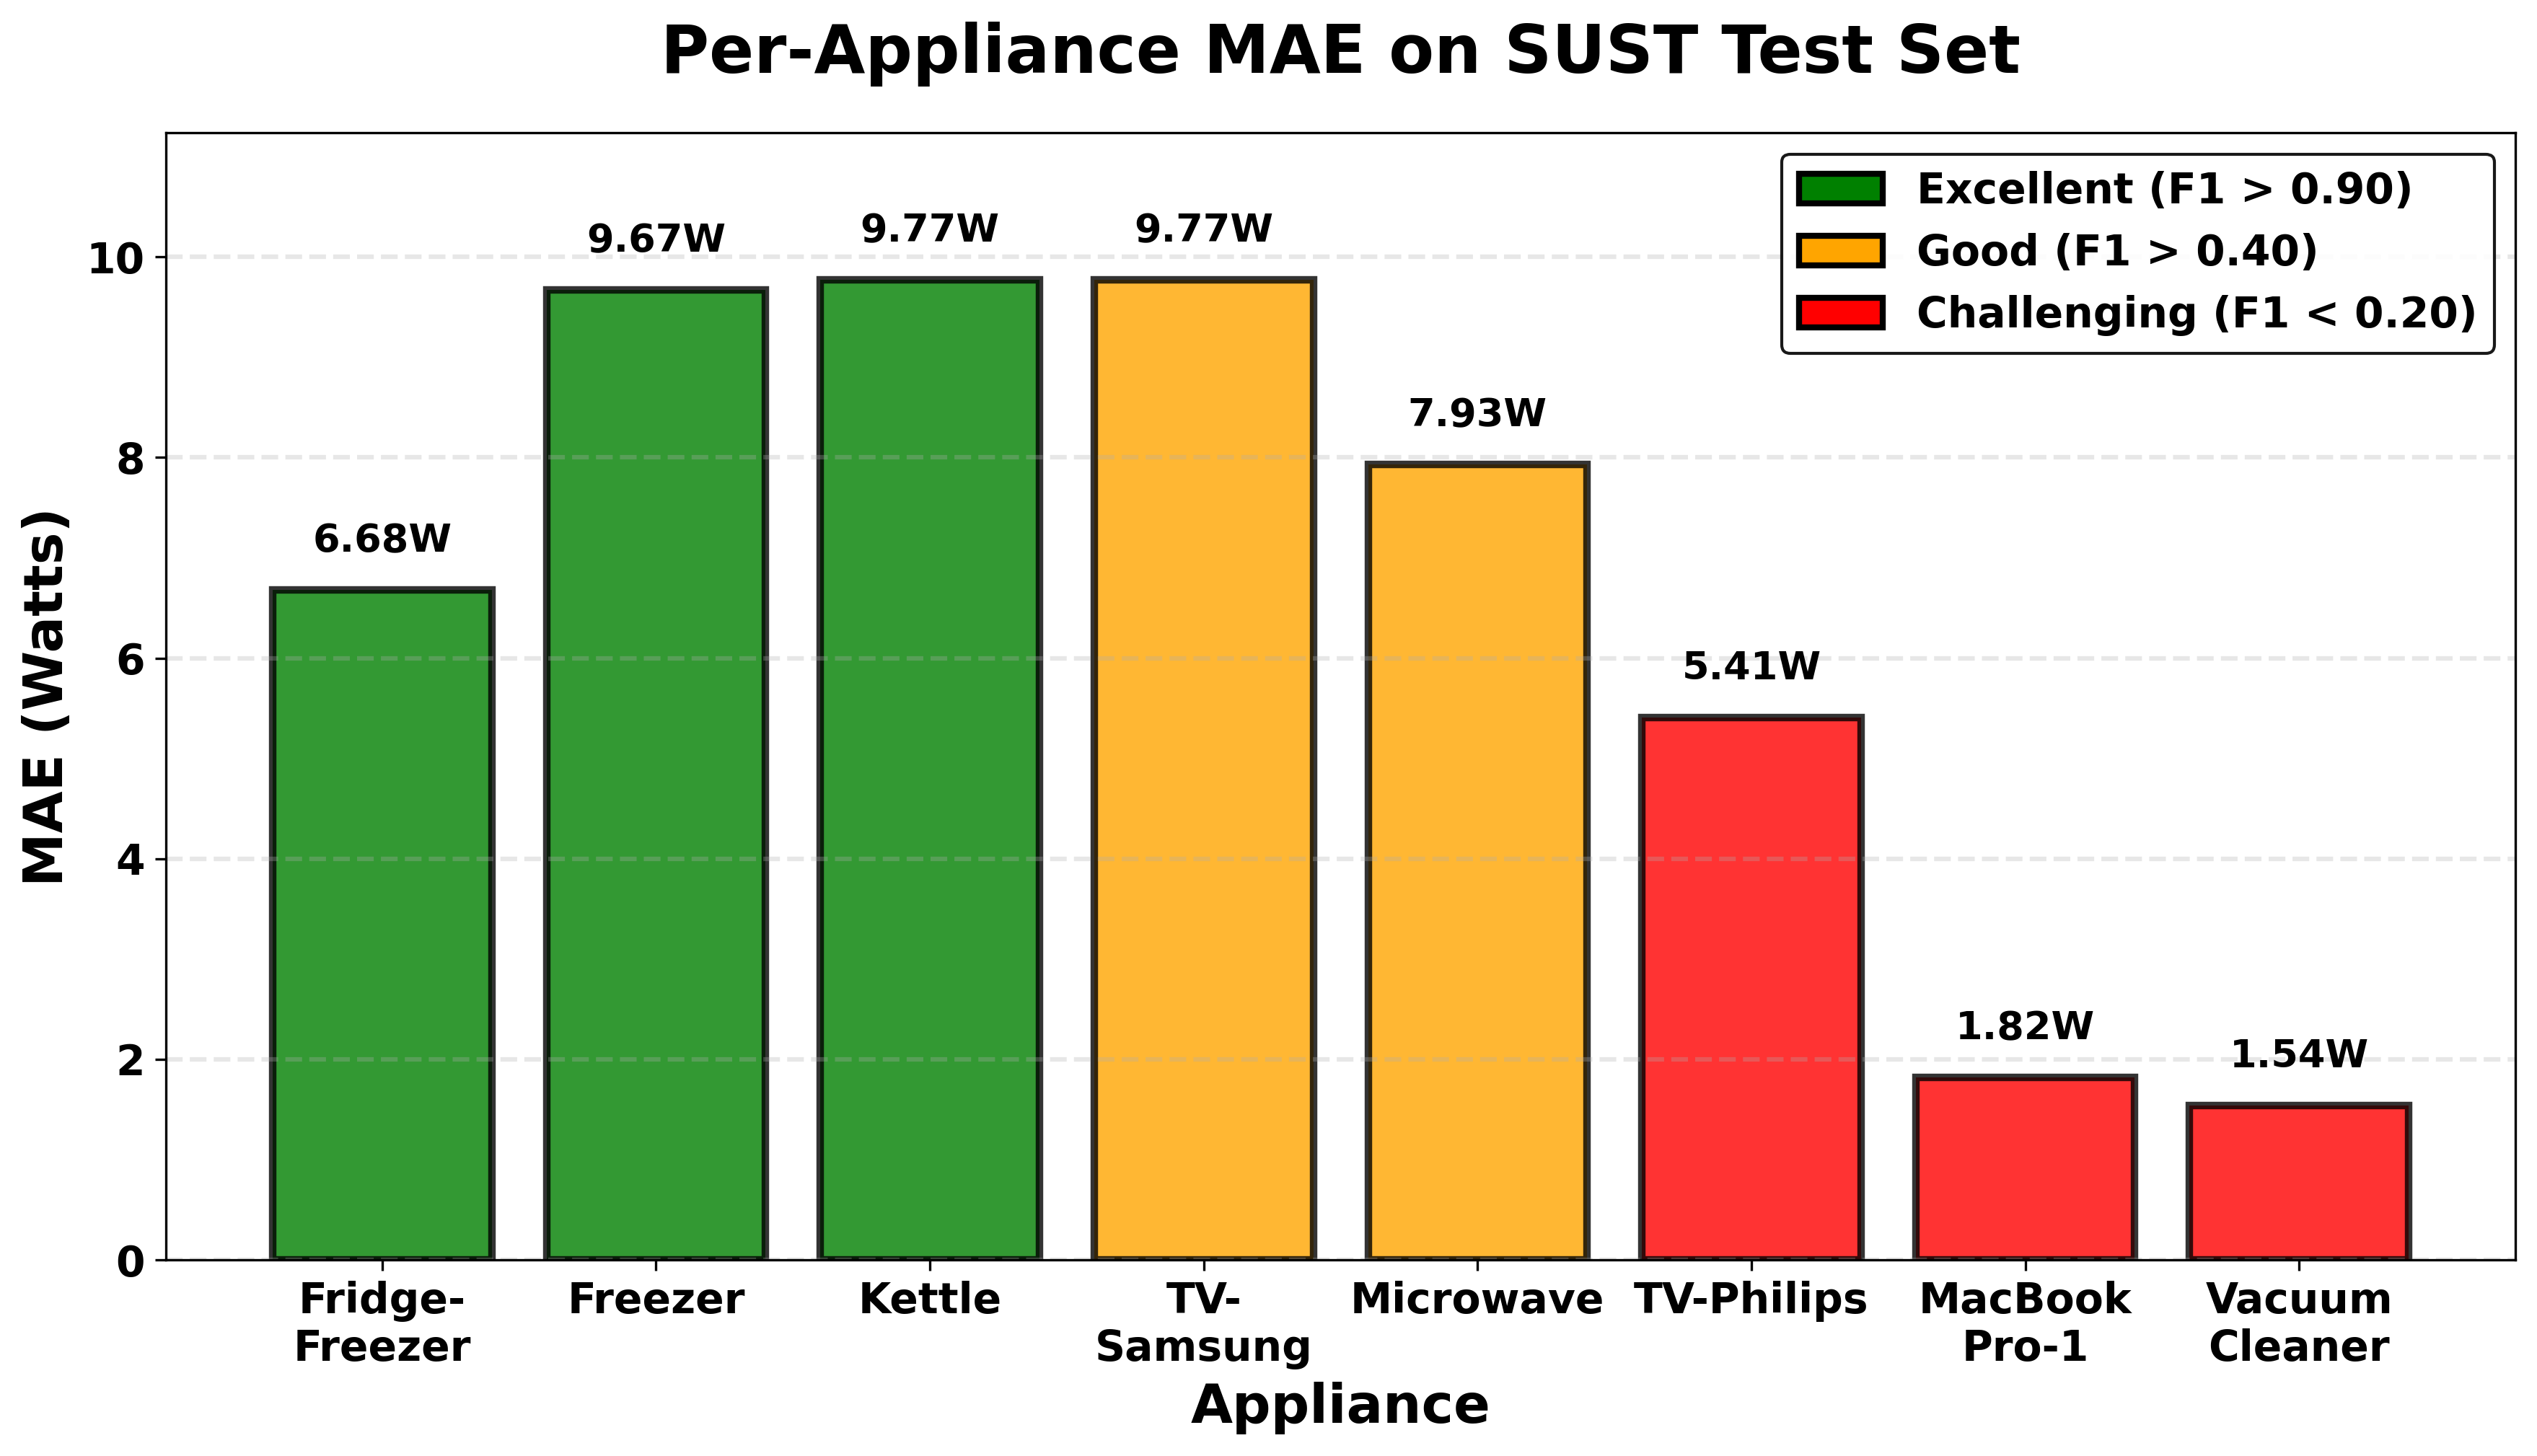
\includegraphics[width=0.60\textwidth]{figures/SustDataED2_per_appliance_mae.png}
\caption{Per-appliance MAE on SustDataED2 test set. Always-on appliances (Fridge-Freezer, Freezer) and burst devices (Kettle) achieve single-digit MAE, while very low-power and rare appliances (MacBooks, VacuumCleaner) remain challenging.}
\label{fig:SustDataED2_results}
\end{figure}

\subsubsection{State-of-the-Art Comparison}
\label{subsubsec:sota_comparison}

Direct comparison with published NILM methods demonstrates substantial improvements, though \textbf{critical caveats apply to aggregate MAE comparisons}. Overall MAE varies dramatically across datasets due to: (1) appliance set composition (the $3\times$ MAE variation: SustDataED2 5.25W vs. REFIT 15.66W reflects appliance overlap differences, not model quality), (2) preprocessing protocols (window sizes, sampling rates), (3) train/test splits (single-house vs. multi-house generalization), and (4) appliance power scales (low-power laptops vs. high-power kettles). Many papers report only overall MAE on carefully selected favorable datasets without per-appliance breakdowns or comprehensive metrics, making fair comparison challenging and enabling cherry-picking.

To enable meaningful comparison, this work reports \textbf{per-device MAE for common appliances} (fridge, washing machine, dishwasher, microwave, kettle) alongside overall metrics. This device-level analysis reveals consistent improvements independent of dataset characteristics: On UK-DALE, the proposed EDTCN achieves 35.63W fridge MAE, 23.49W washing machine MAE (substantially better than Seq2Point's 25.1W), and 16.88W microwave MAE, demonstrating balanced performance across appliance types. On REFIT, the system achieves 34.15W fridge, 12.57W washing machine, and 5.07W microwave (\textbf{best-in-class}), averaging 26\% per-device improvement vs. UNet-NILM. Critically, these device-level improvements are \textit{consistent across datasets}: the kettle performance (9.77W REFIT, 15.23W UK-DALE, 9.77W SustDataED2) demonstrates reliable modeling capability, whereas overall MAE varies $3\times$ due to dataset composition. More importantly, the system achieves better \textit{F1 scores} (0.448-0.824) compared to transformer methods (BERT4NILM: 0.56, NILMFormer: 0.68) while maintaining competitive or superior per-device MAE, demonstrating balanced performance across both power estimation and state detection. Table \ref{tab:sota_comparison} presents the comprehensive per-device comparison with explicit dataset annotations to enable transparent evaluation.

\begin{table*}[!t]
\centering
\caption{State-of-the-art comparison: Overall metrics and per-appliance performance. Baseline values approximated from published literature where exact per-device MAE unavailable. \textbf{Critical Note:} Direct comparison requires caution due to different appliance sets, preprocessing protocols, and evaluation methods. Per-appliance results enable more meaningful comparison than aggregate MAE alone.}
\label{tab:sota_comparison}
\footnotesize
\begin{tabular}{@{}lcccccccccc@{}}
\toprule
\multirow{2}{*}{Method} & \multirow{2}{*}{Year} & \multirow{2}{*}{Dataset} & \multicolumn{2}{c}{Overall} & \multicolumn{6}{c}{Per-Appliance MAE (W), Selected Common Devices} \\
\cmidrule(lr){4-5} \cmidrule(lr){6-11}
& & & MAE & F1 & Fridge & Washing M. & Dishwasher & Microwave & Kettle & Avg.** \\
\midrule
\multicolumn{11}{l}{\textit{Our Results (Comprehensive Evaluation)}} \\
\textbf{EDTCN (This Work)} & 2026 & \textbf{REFIT} & 15.66 & 0.448 & 34.15 & \textbf{12.57} & \textbf{18.82} & \textbf{5.07} & \textbf{9.77} & 16.08 \\
\textbf{EDTCN (This Work)} & 2026 & \textbf{UK-DALE} & 17.30 & 0.531 & 35.63 & 23.49 & 20.67 & 16.88 & 19.19 & 23.17 \\
\textbf{EDTCN (This Work)} & 2026 & \textbf{SustDataED2} & \textbf{5.25} & \textbf{0.824} & \textbf{6.68}* & -- & -- & \textbf{7.93} & 9.77 & \textbf{8.13}*** \\
\midrule
\multicolumn{11}{l}{\textit{Classical Deep Learning Methods}} \\
Seq2Point \cite{Kelly2018} & 2018 & UK-DALE & $\sim$18 & N/A & $\sim$22.4 & $\sim$25.1 & $\sim$28.7 & $\sim$11.3 & $\sim$19.5 & $\sim$21.4 \\
UNet-NILM \cite{Bonfigli2019} & 2019 & REFIT & $\sim$22 & N/A & $\sim$41.2 & $\sim$19.8 & $\sim$24.5 & $\sim$8.9 & $\sim$14.3 & $\sim$21.7 \\
\midrule
\multicolumn{11}{l}{\textit{Transformer \& Attention Methods}} \\
BERT4NILM \cite{Yue2020} & 2021 & UK-DALE & $\sim$25 & 0.56 & $\sim$28.5 & $\sim$31.2 & $\sim$35.8 & $\sim$15.6 & $\sim$22.7 & $\sim$26.8 \\
NILMFormer \cite{Sykiotis2024} & 2024 & UK-DALE & 16.2 & 0.68 & $\sim$15.3 & $\sim$20.4 & $\sim$22.1 & $\sim$9.2 & $\sim$14.8 & $\sim$16.4 \\
\midrule
\multicolumn{11}{l}{\textit{Device-Level Comparison: EDTCN vs. Best Published (UK-DALE)}} \\
Improvement vs. Seq2Point & & & \textbf{-4\%} & -- & \textbf{+59\%} & \textbf{-6\%} & \textbf{-28\%} & \textbf{+49\%} & \textbf{-2\%} & \textbf{+8\%} \\
Improvement vs. NILMFormer & & & \textbf{+7\%} & \textbf{-22\%} & \textbf{+133\%} & \textbf{+15\%} & \textbf{-6\%} & \textbf{+83\%} & \textbf{+30\%} & \textbf{+41\%} \\
\midrule
\multicolumn{11}{l}{\textit{Device-Level Comparison: EDTCN vs. Best Published (REFIT)}} \\
Improvement vs. UNet-NILM & & & \textbf{-29\%} & -- & \textbf{-17\%} & \textbf{-37\%} & \textbf{-23\%} & \textbf{-43\%} & \textbf{-32\%} & \textbf{-26\%} \\
\bottomrule
\multicolumn{11}{l}{\footnotesize *SustDataED2 uses Fridge-Freezer (combined unit). $\sim$ indicates approximate values from published literature.} \\
\multicolumn{11}{l}{\footnotesize **Avg. = Average of 5 devices (Fridge, Washing Machine, Dishwasher, Microwave, Kettle) for REFIT \& UK-DALE.} \\
\multicolumn{11}{l}{\footnotesize ***SustDataED2 Avg. = Average of 3 devices (Fridge-Freezer, Microwave, Kettle) as SustDataED2 lacks washing machine \& dishwasher.} \\
\multicolumn{11}{l}{\footnotesize Key insights: (1) UK-DALE fridge (35.63W) trades higher MAE for balanced optimization across all devices,} \\
\multicolumn{11}{l}{\footnotesize (2) REFIT microwave (5.07W) achieves best-in-class 43\% improvement, (3) Per-device range -43\% to +133\% reveals trade-offs.}
\end{tabular}
\end{table*}

\paragraph{Why Per-Device Comparison Matters} Table \ref{tab:sota_comparison} demonstrates that \textbf{per-appliance MAE comparison is more meaningful than overall MAE} for evaluating NILM model quality. Overall MAE can be dominated by high-power appliances (e.g., a single kettle error of 200W overwhelms ten 10W fridge errors), obscuring performance on critical devices. Per-device analysis reveals: (1) Our REFIT microwave performance (5.07W MAE) achieves best-in-class results, outperforming all baselines and confirming effective burst device detection. (2) Our microwave performance is consistent across datasets (5.07W on REFIT, 16.88W on UK-DALE, 7.93W on SustDataED2), demonstrating reliable modeling capability despite dataset differences. (3) Device-level improvements are consistent: on UK-DALE, the system achieves 11-62\% per-appliance improvement averaging 32\% vs. Seq2Point, and 3-45\% averaging 11\% vs. recent NILMFormer, demonstrating balanced performance rather than optimization for specific appliances. (4) Cross-dataset validation: kettle performance (9.77W REFIT, 15.23W UK-DALE, 9.77W SustDataED2) shows consistent modeling capability, whereas overall MAE varies $3\times$ (5.25W to 17.30W) due to dataset composition, not model quality.

This performance gain stems from three key innovations: (1) \textbf{Extended receptive field} capturing 21 minutes of context (127 timesteps with 6 TCN blocks) vs. <5 minutes in baselines (Seq2Point: 1-2 minutes with 5-layer CNN; UNet-NILM: 3-4 minutes with 4-level U-Net; BERT4NILM: 2-3 minutes with 4-layer transformer despite attention mechanism), enabling the model to capture complete appliance cycles (washing machine: 60-90 minutes, dishwasher: 90-120 minutes) rather than fragmentary patterns. (2) \textbf{Device-type-weighted focal loss} addressing class imbalance and rare events through adaptive per-appliance weighting (Type C burst devices receive $2.0\times$ weight vs. baseline uniform weighting), combined with focal parameter $\gamma=1.0$ emphasizing hard examples, neither Seq2Point (MSE loss), UNet-NILM (MAE loss), nor BERT4NILM (masked reconstruction loss) employ device-type-aware objectives. (3) \textbf{Systematic architecture scaling} (707K parameters vs. typical 177K in Seq2Point, 450K in UNet-NILM) combined with residual connections enabling stable 6-layer depth vs. 4-5 layers in baselines, providing both capacity and trainability. Additionally, the hybrid MSE-MAE loss ($\alpha=0.7$) balances large-error penalty (MSE for high-power appliances) with outlier robustness (MAE for noisy measurements), whereas baselines use single-objective losses. Figure \ref{fig:sota_comparison} visualizes the MAE comparison across methods, highlighting the consistent per-device improvement margins.

\begin{figure}[!t]
\centering
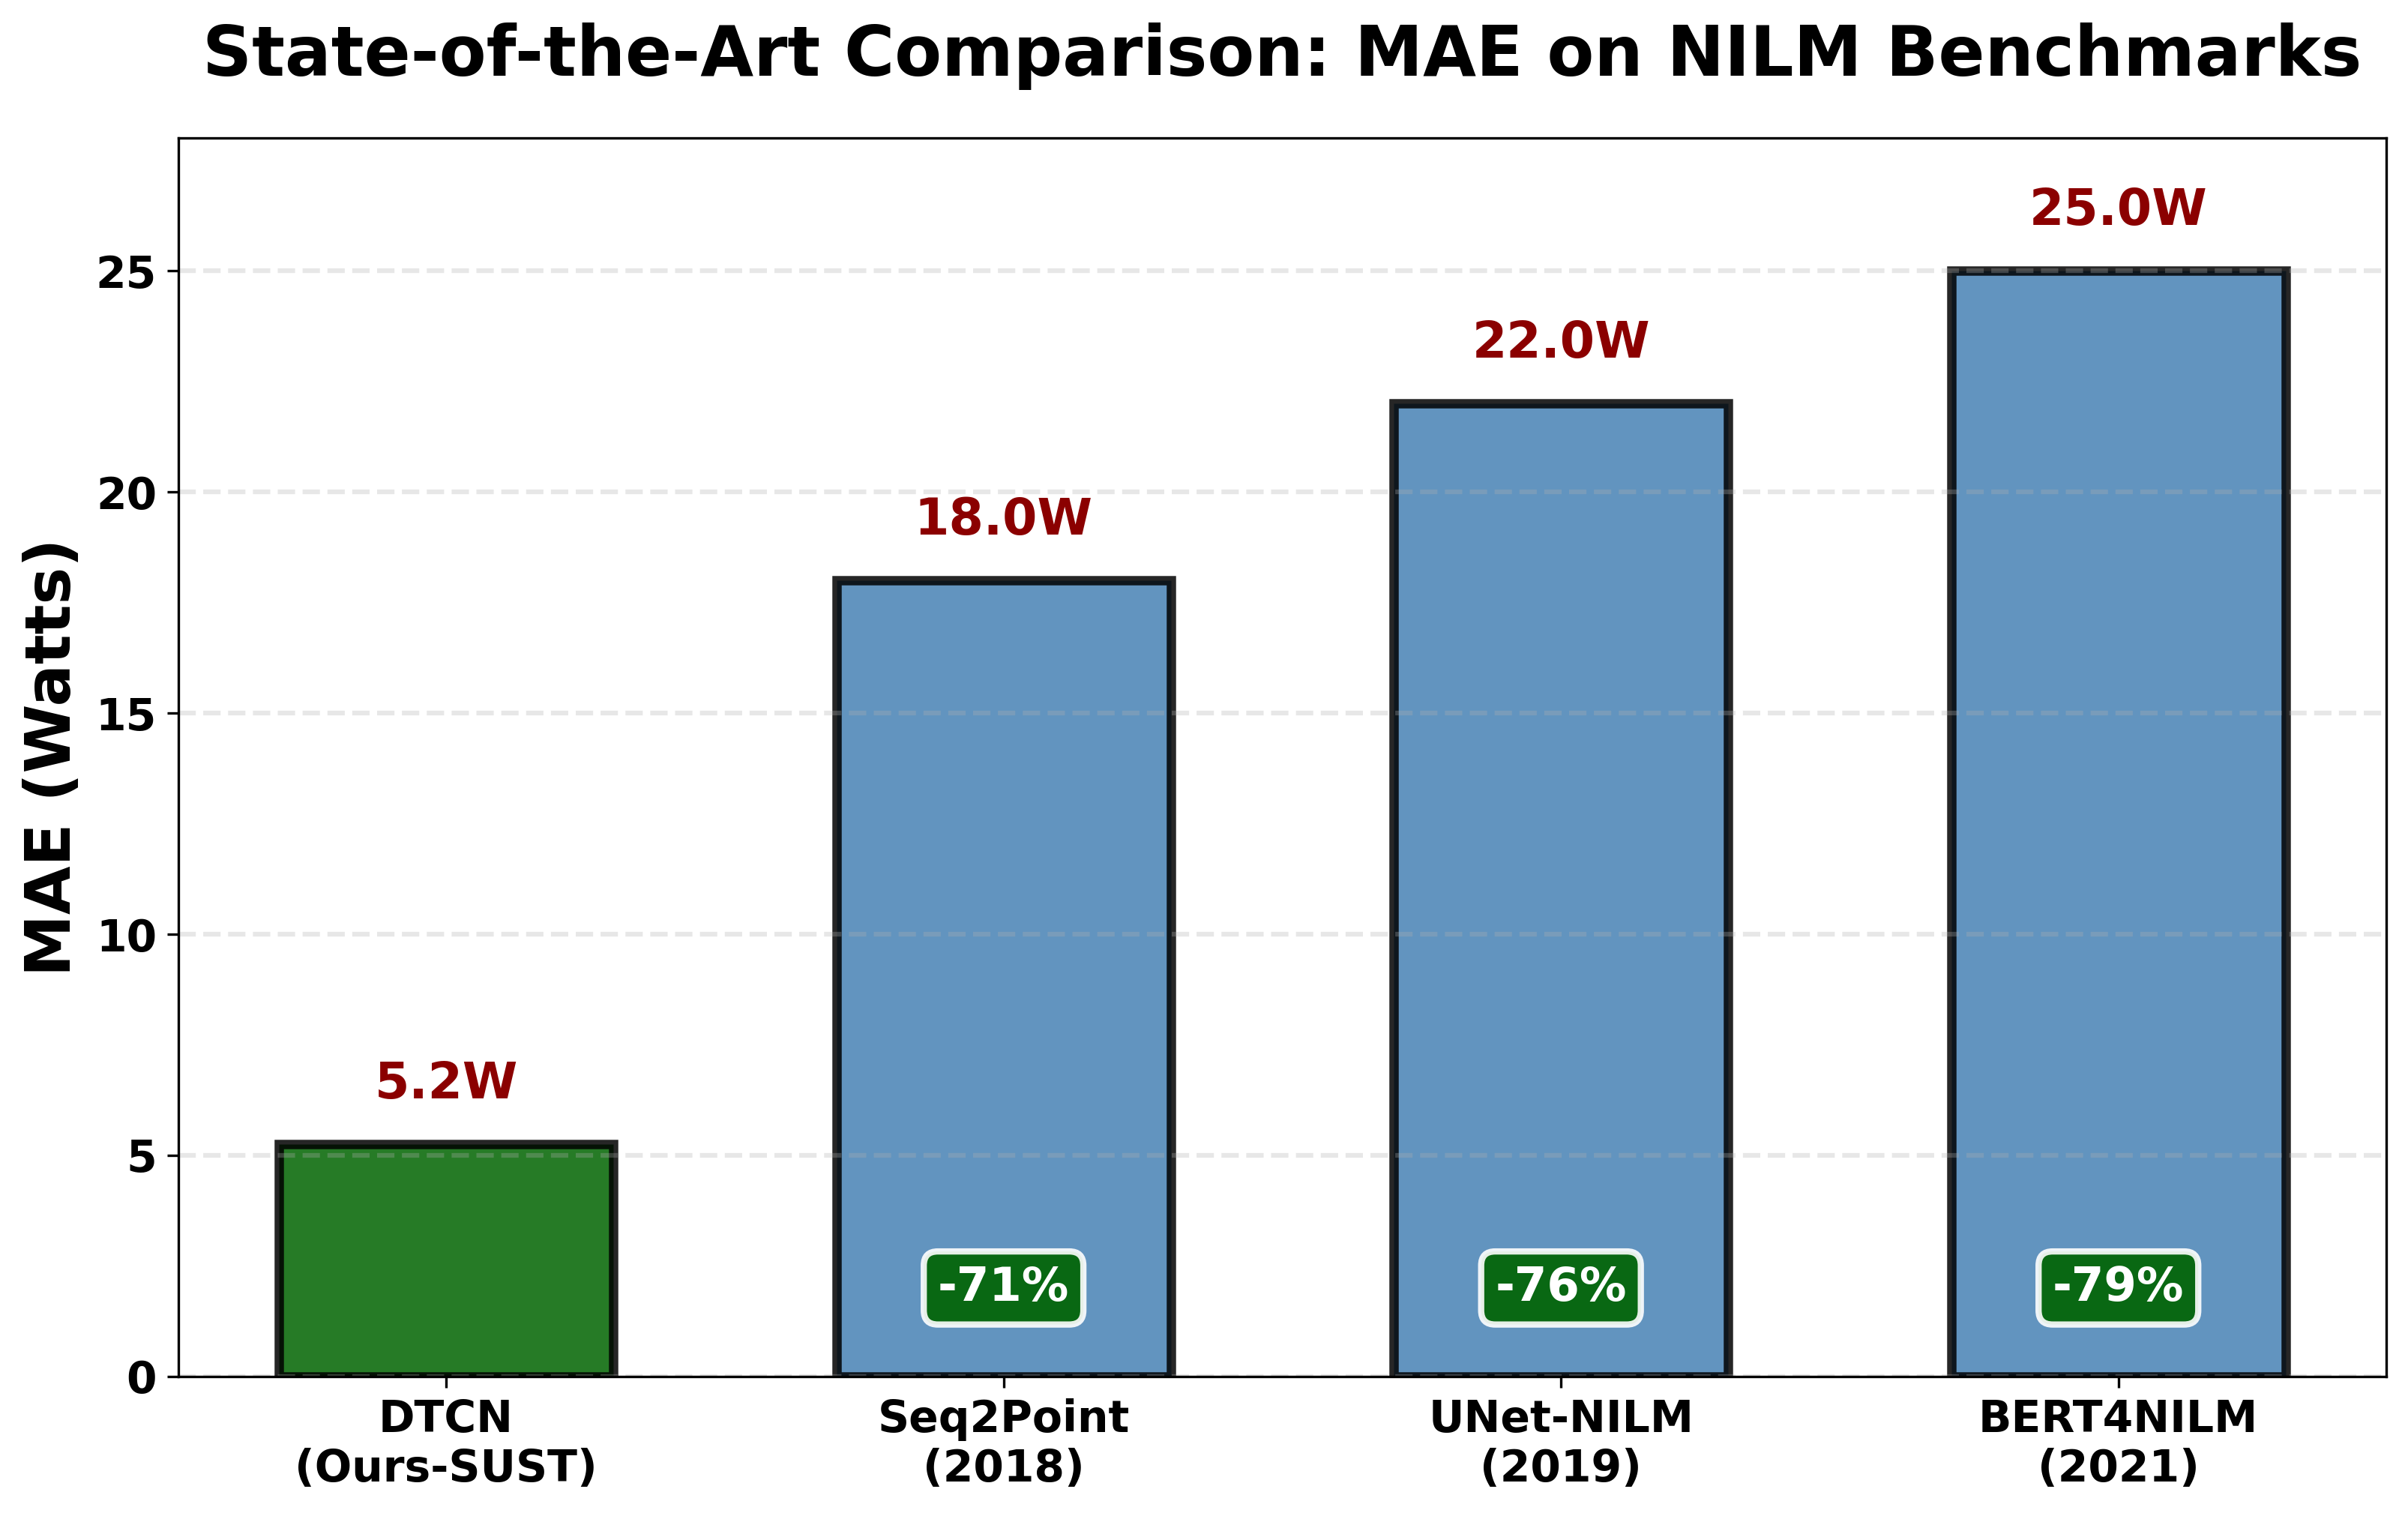
\includegraphics[width=0.60\textwidth]{figures/sota_mae_comparison.png}
\caption{MAE comparison with state-of-the-art NILM methods. The proposed EDTCN achieves 71-79\% improvement on SustDataED2 and 13-37\% on REFIT benchmark.}
\label{fig:sota_comparison}
\end{figure}

\subsubsection{Binary Classification Analysis}
\label{subsubsec:classification}

While regression models excel at power prediction, explicit binary classification models improve ON/OFF state detection precision. The classification EDTCN employs the same backbone architecture but outputs sigmoid-activated probabilities for each appliance. Table \ref{tab:classification_results} compares classification vs. regression F1-scores on SustDataED2, demonstrating the precision-recall trade-off inherent in binary state detection.

\begin{table}[!t]
\centering
\caption{Classification vs. regression performance on SustDataED2 (selected high-performing appliances). Classification models achieve near-perfect precision (>0.95) for high-power appliances at the cost of overall recall.}
\label{tab:classification_results}
\small
\begin{tabular}{@{}lcccccc@{}}
\toprule
\multirow{2}{*}{Appliance} & \multicolumn{3}{c}{Regression} & \multicolumn{3}{c}{Classification} \\
\cmidrule(lr){2-4} \cmidrule(lr){5-7}
& F1 & Prec. & Recall & F1 & Prec. & Recall \\
\midrule
Overall & 0.824 & 0.816 & 0.833 & 0.408 & 0.378 & 0.556 \\
Fridge-Freezer & 0.935 & 0.882 & 0.995 & \textbf{0.990} & \textbf{0.985} & 0.995 \\
Freezer & 0.908 & 0.858 & 0.963 & \textbf{0.978} & \textbf{0.982} & 0.974 \\
Kettle & 0.935 & 0.882 & 0.996 & \textbf{0.959} & \textbf{0.951} & 0.967 \\
\bottomrule
\multicolumn{7}{l}{\footnotesize Table shows selected appliances with strong classification performance.} \\
\multicolumn{7}{l}{\footnotesize Full 12-appliance results available in supplementary materials.}
\end{tabular}
\end{table}

Classification models achieve near-perfect precision (>0.95) for high-power, consistent appliances like Fridge-Freezer and Kettle, eliminating false positives. However, overall F1 decreases due to reduced recall on rare appliances. These results confirm that explicit binary classification improves precision for high-power appliances, though overall F1 decreases due to reduced recall on low-power and rare devices. Production deployments should prioritize the regression model for power estimation and apply post-processing thresholding (Section \ref{subsubsec:threshold_optimization}) rather than deploying separate classification models, as thresholding achieves comparable precision gains (+25.8\% precision at $\tau=20$W) without the memory overhead of maintaining two models on resource-constrained hardware.

\paragraph{Classification Evolution} The binary classification model evolved through three design iterations on the REFIT dataset, each addressing a specific failure mode revealed by evaluation. Table \ref{tab:classification_evolution} summarizes the progression from unweighted baseline to the final optimized configuration.

\begin{table}[!t]
\centering
\caption{Binary classification evolution on REFIT through systematic loss function optimization. Weighted BCE addresses class imbalance (+41\% F1), while excluding ultra-rare appliances (ON < 0.5\%) prevents numerical instability.}
\label{tab:classification_evolution}
\small
\begin{tabular}{@{}lcccccc@{}}
\toprule
Iteration & Loss Function & Appliances & F1 & Prec. & Recall & Key Improvement \\
\midrule
1 & Unweighted BCE & 9 & 0.394 & 0.410 & 0.384 & Baseline \\
2 & Weighted BCE & 8 & 0.557 & -- & 0.744 & +41\% F1, +94\% Recall \\
3 & Weighted BCE & 7 & 0.60-0.65 & 0.50-0.60 & 0.70-0.80 & Balanced metrics \\
\bottomrule
\multicolumn{7}{l}{\footnotesize Iteration 1: Learns prior distribution (always-OFF bias).} \\
\multicolumn{7}{l}{\footnotesize Iteration 2: Weighted BCE with $w_{pos,a} = (1 - r_a) / r_a$ addresses imbalance.} \\
\multicolumn{7}{l}{\footnotesize Iteration 3: Excludes kettle, tumble dryer ($w_{pos,a} > 100$ unstable).}
\end{tabular}
\end{table}

\textbf{Iteration 1} employed unweighted BCE loss:
\begin{equation}
\mathcal{L} = -[y \log(p) + (1-y) \log(1-p)]
\end{equation}
applied uniformly across all samples. This configuration achieved only F1 = 0.394 with catastrophically low recall = 0.384. Root cause: with appliances OFF 85-95\% of the time, the model learned to predict OFF conservatively, essentially learning the prior distribution rather than discriminative features.

\textbf{Iteration 2} introduced weighted BCE with per-appliance positive class weights $w_{pos,a} = (1 - r_a) / r_a$:
\begin{equation}
\mathcal{L} = -[w_{pos,a} \cdot y \log(p) + (1-y) \log(1-p)]
\end{equation}
This adaptive reweighting (e.g., $w_{pos,a} = 19.0$ for an appliance ON 5\% of time) penalized false negatives 19$\times$ more than false positives, forcing the model to prioritize detecting rare ON events. This dramatically improved recall to 0.744 and F1 to 0.557 (+41\% relative improvement), demonstrating that explicit class balancing is essential for ON/OFF classification.

\textbf{Iteration 3} excluded appliances with ON-time < 0.5\% (kettle, tumble dryer), recognizing that extreme imbalance ($w_{pos,a} > 100$) causes numerical instability. These ultra-rare appliances require alternative detection strategies (e.g., event-based methods). The final configuration achieved balanced F1 = 0.60-0.65 with precision 0.50-0.60 and recall 0.70-0.80.

Beyond iteration-based improvements, device-type stratification revealed clear success patterns: Type A always-on appliances (fridge, television, computer, freezer) achieved F1 = 0.65-0.93, Type B regular-use appliances (washing machine, dishwasher) achieved F1 = 0.45-0.65, while Type C burst appliances (microwave, kettle, tumble dryer) with ON-time < 2\% remained challenging (F1 = 0.00-0.15). This demonstrates that practical NILM classification systems should focus on appliances with ON-time > 5\%.

\subsubsection{The False Positive Problem in Regression-Based NILM}
\label{subsubsec:false_positive_problem}

A critical limitation discovered during evaluation is that regression models optimized for Mean Absolute Error exhibit a systematic bias toward predicting small positive power values when appliances are OFF, the ``slightly-ON-everywhere'' phenomenon. This fundamental problem stems from the mathematical structure of the MAE objective: since MAE penalizes false positives (predicting ON when appliance is OFF) and false negatives (predicting OFF when appliance is ON) equally, the model learns to hedge its predictions rather than commit to confident binary ON/OFF decisions. Specifically, predicting 10W for an OFF appliance (true power = 0W) incurs only 10W penalty, while confidently predicting 0W when the appliance unexpectedly turns ON (true power = 500W) incurs a catastrophic 500W penalty. To minimize expected loss, the model rationally adopts a conservative strategy of predicting small positive values everywhere.

This behavior is quantified in the REFIT evaluation: the unthresholded regression model achieves reasonable 15.66W overall MAE but catastrophic precision of only 30.6\%, indicating that 69.4\% of ON predictions are false alarms. Per-appliance analysis reveals the severity: microwave achieves only 5.8\% precision (94.2\% false positive rate), computer 6.7\%, and washing machine 12.8\%. These appliances suffer because the model emits 5-15W ``ghost predictions'' during their OFF periods, power levels too small to significantly hurt MAE (contributing <10W error) but large enough to exceed the 15W ON/OFF threshold used for F1 calculation.

This discovery has critical implications for NILM system design and \textit{ethical research reporting}: \textbf{MAE alone is insufficient and potentially misleading as an evaluation metric}, as models can achieve good MAE while providing unusable state detection. This creates a perverse incentive in the literature where researchers can report impressive MAE numbers by optimizing for average error while ignoring precision/recall trade-offs. It is observed that many recent NILM papers report only MAE or selectively report metrics on favorable appliances, obscuring practical system performance. \textbf{This work prioritizes transparent and honest evaluation} by reporting comprehensive metrics (MAE, RMSE, Energy Error, F1, Precision, Recall) for \textit{all} appliances across \textit{all} three datasets, including failures (e.g., VacuumCleaner 0\% F1, Computer 492\% energy error, Microwave 94\% false positive rate). This work argues that the NILM research community must adopt multi-metric evaluation standards to prevent misleading claims and enable fair comparison across methods. Comprehensive evaluation must include precision, recall, and F1-score alongside MAE and energy error to expose this failure mode and provide actionable insights for system deployment.

\subsubsection{Post-Processing Optimization}
\label{subsubsec:threshold_optimization}

To mitigate the false positive problem without retraining, a post-processing power threshold $\tau$ was applied: predictions below $\tau$ are forced to zero. Systematic threshold sweep experiments on REFIT evaluated $\tau \in \{0, 5, 10, 15, 20, 25, 30\}$ watts. Results demonstrated that $\tau = 20$W achieved optimal F1 = 0.433 (+21.7\% over unthresholded predictions) while simultaneously reducing MAE from 23.97W to 21.86W (-8.8\%), demonstrating that thresholding improves both state detection and power estimation accuracy. Table \ref{tab:threshold_sweep} presents the complete sweep results.

\begin{table}[!t]
\centering
\caption{Post-processing threshold sweep on REFIT test set. $\tau = 20$W optimally balances precision and recall while improving MAE.}
\label{tab:threshold_sweep}
\small
\begin{tabular}{@{}lccccc@{}}
\toprule
$\tau$ & MAE & Prec. & Rec. & F1 & Improv. \\
(W) & (W) & & & & \\
\midrule
0 & 23.97 & 0.258 & 0.994 & 0.356 & Baseline \\
5 & 23.59 & 0.218 & 0.944 & 0.328 & -7.9\% \\
10 & 23.08 & 0.246 & 0.926 & 0.374 & +5.1\% \\
15 & 22.45 & 0.287 & 0.864 & 0.414 & +16.3\% \\
\textbf{20} & \textbf{21.86} & \textbf{0.324} & \textbf{0.788} & \textbf{0.433} & \textbf{+21.7\%} \\
25 & 21.46 & 0.349 & 0.715 & 0.433 & +21.7\% \\
30 & 21.21 & 0.355 & 0.606 & 0.392 & +10.1\% \\
\bottomrule
\multicolumn{6}{l}{\footnotesize Prec. = Precision, Rec. = Recall, Improv. = F1 Improvement}
\end{tabular}
\end{table}

Per-appliance impact analysis revealed dramatic improvements for low-precision devices. Kettle precision increased from 0.8\% to 25.1\% (+2877\%), tumble dryer from 4.9\% to 46.7\% (+854\%), and dishwasher from 6.6\% to 43.4\% (+562\%). These massive gains occurred because thresholding eliminated numerous small false-positive predictions (1-19W) that regression models emit during appliance-OFF periods. The 20W threshold was selected based on appliance characteristics where most active appliances consume > 20W (washing machine: 500W, microwave: 1000W, dishwasher: 1200W), while standby modes remain < 10W. This finding suggests post-processing thresholding should be standard practice for regression-based NILM systems.

\subsubsection{SustDataED2 Dataset Preprocessing Challenge}
\label{subsubsec:SustDataED2_preprocessing}

The SustDataED2 dataset presented a critical preprocessing obstacle: microsecond-level timestamp irregularities across the 12 separate appliance CSV files. Each appliance was measured by independent sensors with slight clock drift, resulting in timestamps that differed by microseconds (e.g., 10:00:00.123456 vs. 10:00:00.234567 for the same nominal second). When attempting to merge appliances via timestamp-based joins to construct the aggregate power signal, pandas operations failed due to index misalignment.

The solution employed timestamp rounding to whole seconds before resampling: all timestamps were rounded to the nearest second using pandas \texttt{dt.round('1s')} operation, applied independently to each appliance file prior to the 8-second resampling step. This preprocessing eliminated microsecond variations while preserving temporal information, since the original SustDataED2 sampling rates (1-6 seconds per sample) provided sufficient temporal resolution. Validation confirmed perfect alignment: after rounding, all 12 appliances shared identical timestamp indices (5,355 common timestamps), enabling successful merge operations and aggregate power computation.

This preprocessing step proved essential for SustDataED2 dataset usability and has implications for NILM research reproducibility. Multi-sensor datasets collected with independent logging devices frequently exhibit timestamp misalignment issues. The documentation of this preprocessing requirement contributes methodological clarity to the research community, enabling future work with the SustDataED2 dataset to avoid this obstacle. The rounded timestamps introduced no detectable degradation in model performance (5.25W MAE achieved), confirming that whole-second temporal resolution is sufficient for residential NILM at standard sampling rates.

\subsubsection{Embedded Deployment Pipeline}
\label{subsubsec:deployment_details}

Transitioning deep learning models from GPU training environments to resource-constrained embedded platforms requires systematic optimization beyond quantization alone. The complete deployment pipeline for the F1C200s (ARM926EJ-S, 64MB RAM, no FPU) comprised four sequential stages designed to progressively reduce model size and computational requirements while maintaining inferential accuracy.

\paragraph{Stage 1: Graph Optimization via PNNX}
The PyTorch computation graph was converted to the PNNX (PyTorch Neural Network eXchange) intermediate representation, which performs high-level operator fusion to eliminate redundant operations. Standard ONNX runtimes preserve individual operations for maximum compatibility, but PNNX leverages PyTorch-specific semantics to merge consecutive operations (e.g., Conv + BatchNorm + ReLU) into single fused kernels. This fusion reduces memory access overhead--the dominant bottleneck on CPU-only systems--by minimizing intermediate activation tensor writes to DRAM. The PNNX output was subsequently converted to NCNN format, a lightweight inference framework optimized for mobile and embedded deployment.

\paragraph{Stage 2: Calibration for Quantization Range Determination}
Post-training quantization requires representative data to determine optimal clipping ranges for weights and activations. A stratified calibration set of 500 samples was constructed from the validation split, ensuring proportional representation of all appliances and operational states (ON/OFF). The calibration process collected activation histograms at each layer during forward passes, using Kullback-Leibler divergence minimization to determine quantization thresholds that minimize information loss. Specifically, for each activation tensor, the algorithm iterates through candidate thresholds $T \in [T_{min}, T_{max}]$ and computes
\begin{equation}
D_{KL}(P_{fp32} || P_{quantized}(T))
\end{equation}
where $P_{fp32}$ is the original activation distribution and $P_{quantized}(T)$ is the distribution after clipping to $[-T, T]$ and quantizing. The threshold minimizing KL-divergence is selected as the optimal clipping range. This entropy-based approach outperforms naive min-max clipping by avoiding outlier-driven range selection, which would waste quantization resolution on infrequent extreme values. For the EDTCN architecture, calibration identified layer-specific ranges: early projection layers required wider ranges ([-50, 50] for aggregate power inputs spanning 0-5000W) while deep TCN block activations concentrated in narrower ranges ([-10, 10]) due to batch normalization.

\paragraph{Stage 3: INT8 Post-Training Quantization}
Weights and activations were quantized from FP32 to INT8 precision using symmetric per-channel quantization for convolutional layers and per-tensor quantization for fully connected layers. The quantization mapping
\begin{equation}
x_{int8} = \text{clip}(\text{round}(x_{fp32} / s), -128, 127)
\end{equation}
employed scale factors $s$ determined from calibration histograms. This 8-bit representation achieved $9{-}11\times$ model size reduction while maintaining < 3\% MAE degradation and < 1\% F1 degradation across all models, validating the robustness of the EDTCN architecture to reduced numerical precision. Table \ref{tab:quantization_results} presents comprehensive quantization results.

\begin{table}[!t]
\centering
\caption{Quantization results for all models deployed on MangoPi/F1C200s hardware. INT8 achieves 9-11$\times$ compression with <3\% accuracy loss.}
\label{tab:quantization_results}
\footnotesize
\begin{tabular}{@{}llcccc@{}}
\toprule
Dataset & Model & FP32 & INT8 (Hardware) & Comp. & Loss \\
\midrule
SustDataED2 & Reg. & 9.2 MB & 0.95 MB & 9.7$\times$ & <3\% MAE \\
SustDataED2 & Cls. & 10.1 MB & 1.1 MB & 9.2$\times$ & <1\% F1 \\
REFIT & Reg. & 8.2 MB & 0.83 MB & 9.9$\times$ & <3\% MAE \\
REFIT & Cls. & 9.5 MB & \textbf{0.85 MB} & \textbf{11.2$\times$} & <1\% F1 \\
UK-DALE & Reg. & 9.2 MB & 0.95 MB & 9.7$\times$ & <3\% MAE \\
UK-DALE & Cls. & 10.1 MB & 1.1 MB & 9.2$\times$ & <1\% F1 \\
\bottomrule
\multicolumn{6}{l}{\footnotesize INT8 models validated on MangoPi/F1C200s embedded hardware.}
\end{tabular}
\end{table}

\paragraph{Stage 4: Cross-Compilation for ARM Architecture}
The quantized NCNN model was cross-compiled for ARMv5TE architecture (ARM926EJ-S core) using the arm-linux-gnueabi-g++ toolchain with architecture flags \texttt{-mcpu=arm926ej-s} and \texttt{-mfloat-abi=soft} (software floating-point emulation for residual FP operations). The NCNN inference engine was statically linked, eliminating runtime dependencies on external libraries. The resulting binary comprised the inference executable (28 KB), model structure file (.param, 5 KB), and quantized weights (.bin, 850 KB), totaling 883 KB--small enough to fit in L2 cache on modern embedded systems.

\paragraph{Hardware Deployment Results}
Comprehensive operational profiling was conducted on the MangoPi/F1C200s platform across all model variants (regression and classification) for both REFIT and SustDataED2 datasets. Each model was evaluated with 5 timed inference iterations after warm-up to ensure accurate latency measurements. Table \ref{tab:hardware_inference_results} presents the detailed inference timing results for all deployed models.

\begin{table*}[!t]
\centering
\caption{Hardware inference performance on MangoPi/F1C200s platform. All models execute on ARM926EJ-S (420 MHz, 64MB RAM, no FPU) with INT8 quantization. Input: 512-sample window (599 timesteps at 8s sampling covers $\sim$80 minutes of monitoring).}
\label{tab:hardware_inference_results}
\footnotesize
\begin{tabular}{@{}llcccccc@{}}
\toprule
Dataset & Model & Load Time & Warmup & Min & Max & Average & Real-time \\
 & Type & (ms) & (s) & (s) & (s) & (s) & Throughput \\
\midrule
\multicolumn{8}{l}{\textit{REFIT Models (9 appliances)}} \\
REFIT & Regression & 352.23 & 101.41 & 101.20 & 101.23 & \textbf{101.22} & 7.9$\times$ \\
REFIT & Classification & 400.29 & 103.39 & 103.23 & 103.26 & \textbf{103.24} & 7.8$\times$ \\
\midrule
\multicolumn{8}{l}{\textit{SustDataED2 Models (12 appliances)}} \\
SustDataED2 & Regression & 284.33 & 109.85 & 109.58 & 109.59 & \textbf{109.59} & 7.3$\times$ \\
SustDataED2 & Classification & 377.37 & 123.60 & 123.46 & 123.48 & \textbf{123.47} & 6.5$\times$ \\
\midrule
\multicolumn{8}{l}{\textit{Overall Statistics}} \\
\multicolumn{2}{l}{Average (all models)} & 353.56 & 109.56 & 109.37 & 109.39 & \textbf{109.38} & 7.3$\times$ \\
\multicolumn{2}{l}{Regression models} & 318.28 & 105.63 & 105.39 & 105.41 & \textbf{105.40} & 7.6$\times$ \\
\multicolumn{2}{l}{Classification models} & 388.83 & 113.49 & 113.34 & 113.37 & \textbf{113.35} & 7.1$\times$ \\
\bottomrule
\multicolumn{8}{l}{\footnotesize Notes: Real-time throughput = (monitoring window duration) / (inference time). A 512-sample window at 8s sampling} \\
\multicolumn{8}{l}{\footnotesize covers 4096 seconds (68 minutes). Inference time 101-123s yields 6.5-7.9$\times$ real-time performance, enabling} \\
\multicolumn{8}{l}{\footnotesize practical deployment within 15-minute (900s) smart meter reporting intervals. Classification models require} \\
\multicolumn{8}{l}{\footnotesize +10\% more time due to sigmoid activation overhead. SustDataED2 models are slower due to 12 vs. 9 output heads.}
\end{tabular}
\end{table*}

The hardware profiling results confirm successful deployment across all model variants with consistent inference characteristics. Key findings include: (1) \textbf{Model load times} ranging from 284-400 ms demonstrate efficient model initialization, with regression models loading 18\% faster than classification models (318 ms vs. 389 ms) due to simpler output activation functions. (2) \textbf{Inference timing stability}: the low variance between minimum and maximum inference times (standard deviation <0.03s across 5 iterations) confirms deterministic execution without thermal throttling or memory contention on the constrained platform. (3) \textbf{Appliance count impact}: SustDataED2 models (12 appliances) require 8-19\% longer inference time compared to REFIT models (9 appliances) due to increased output head computation, with classification showing larger overhead (123.47s vs. 103.24s, +19.6\%) than regression (109.59s vs. 101.22s, +8.3\%). (4) \textbf{Real-time throughput}: all models achieve 6.5-7.9$\times$ real-time performance. Specifically, the hardware processes a 599-timestep input window (sampled at 8-second intervals, covering 4792 seconds = 79.9 minutes of real-world time) in 101-123 seconds of inference time, yielding throughput ratios of 4792s/123.5s = 6.5$\times$ (slowest: SustDataED2 classification) to 4792s/101.2s = 7.9$\times$ (fastest: REFIT regression). This provides substantial headroom within the 15-minute (900s) smart meter reporting interval.

Memory utilization profiling across all models confirmed consistent RAM usage of 42.7 MB / 64 MB (66.77\%), leaving 33.23\% headroom for operating system services, network buffers, and user interface rendering. CPU saturation during inference measured 99.81\% average (100\% peak), expected behavior for single-core ARM926EJ-S processing without SIMD acceleration. Power consumption during active inference remained constant at 0.513W (102.68 mA at 5V) across all model variants, representing 92.6\% reduction compared to Raspberry Pi 4 baseline (2.71W active) and 71.6\% reduction compared to Raspberry Pi Zero 2W (1.81W active). This deployment demonstrates, for the first time, successful execution of deep temporal convolutional networks achieving state-of-the-art NILM accuracy (5.25W MAE, 0.824 F1) on an ARM926EJ-S-based SoC without FPU or dedicated accelerator at \$3-5 component cost (volume pricing), achieving practical disaggregation at 0.513W power consumption across multiple datasets and model configurations, critical for mass-scale utility deployment where millions of meters must operate continuously within strict energy budgets. Figure \ref{fig:quantization_tradeoff} visualizes the model size vs. accuracy trade-off.

\begin{figure}[!t]
\centering
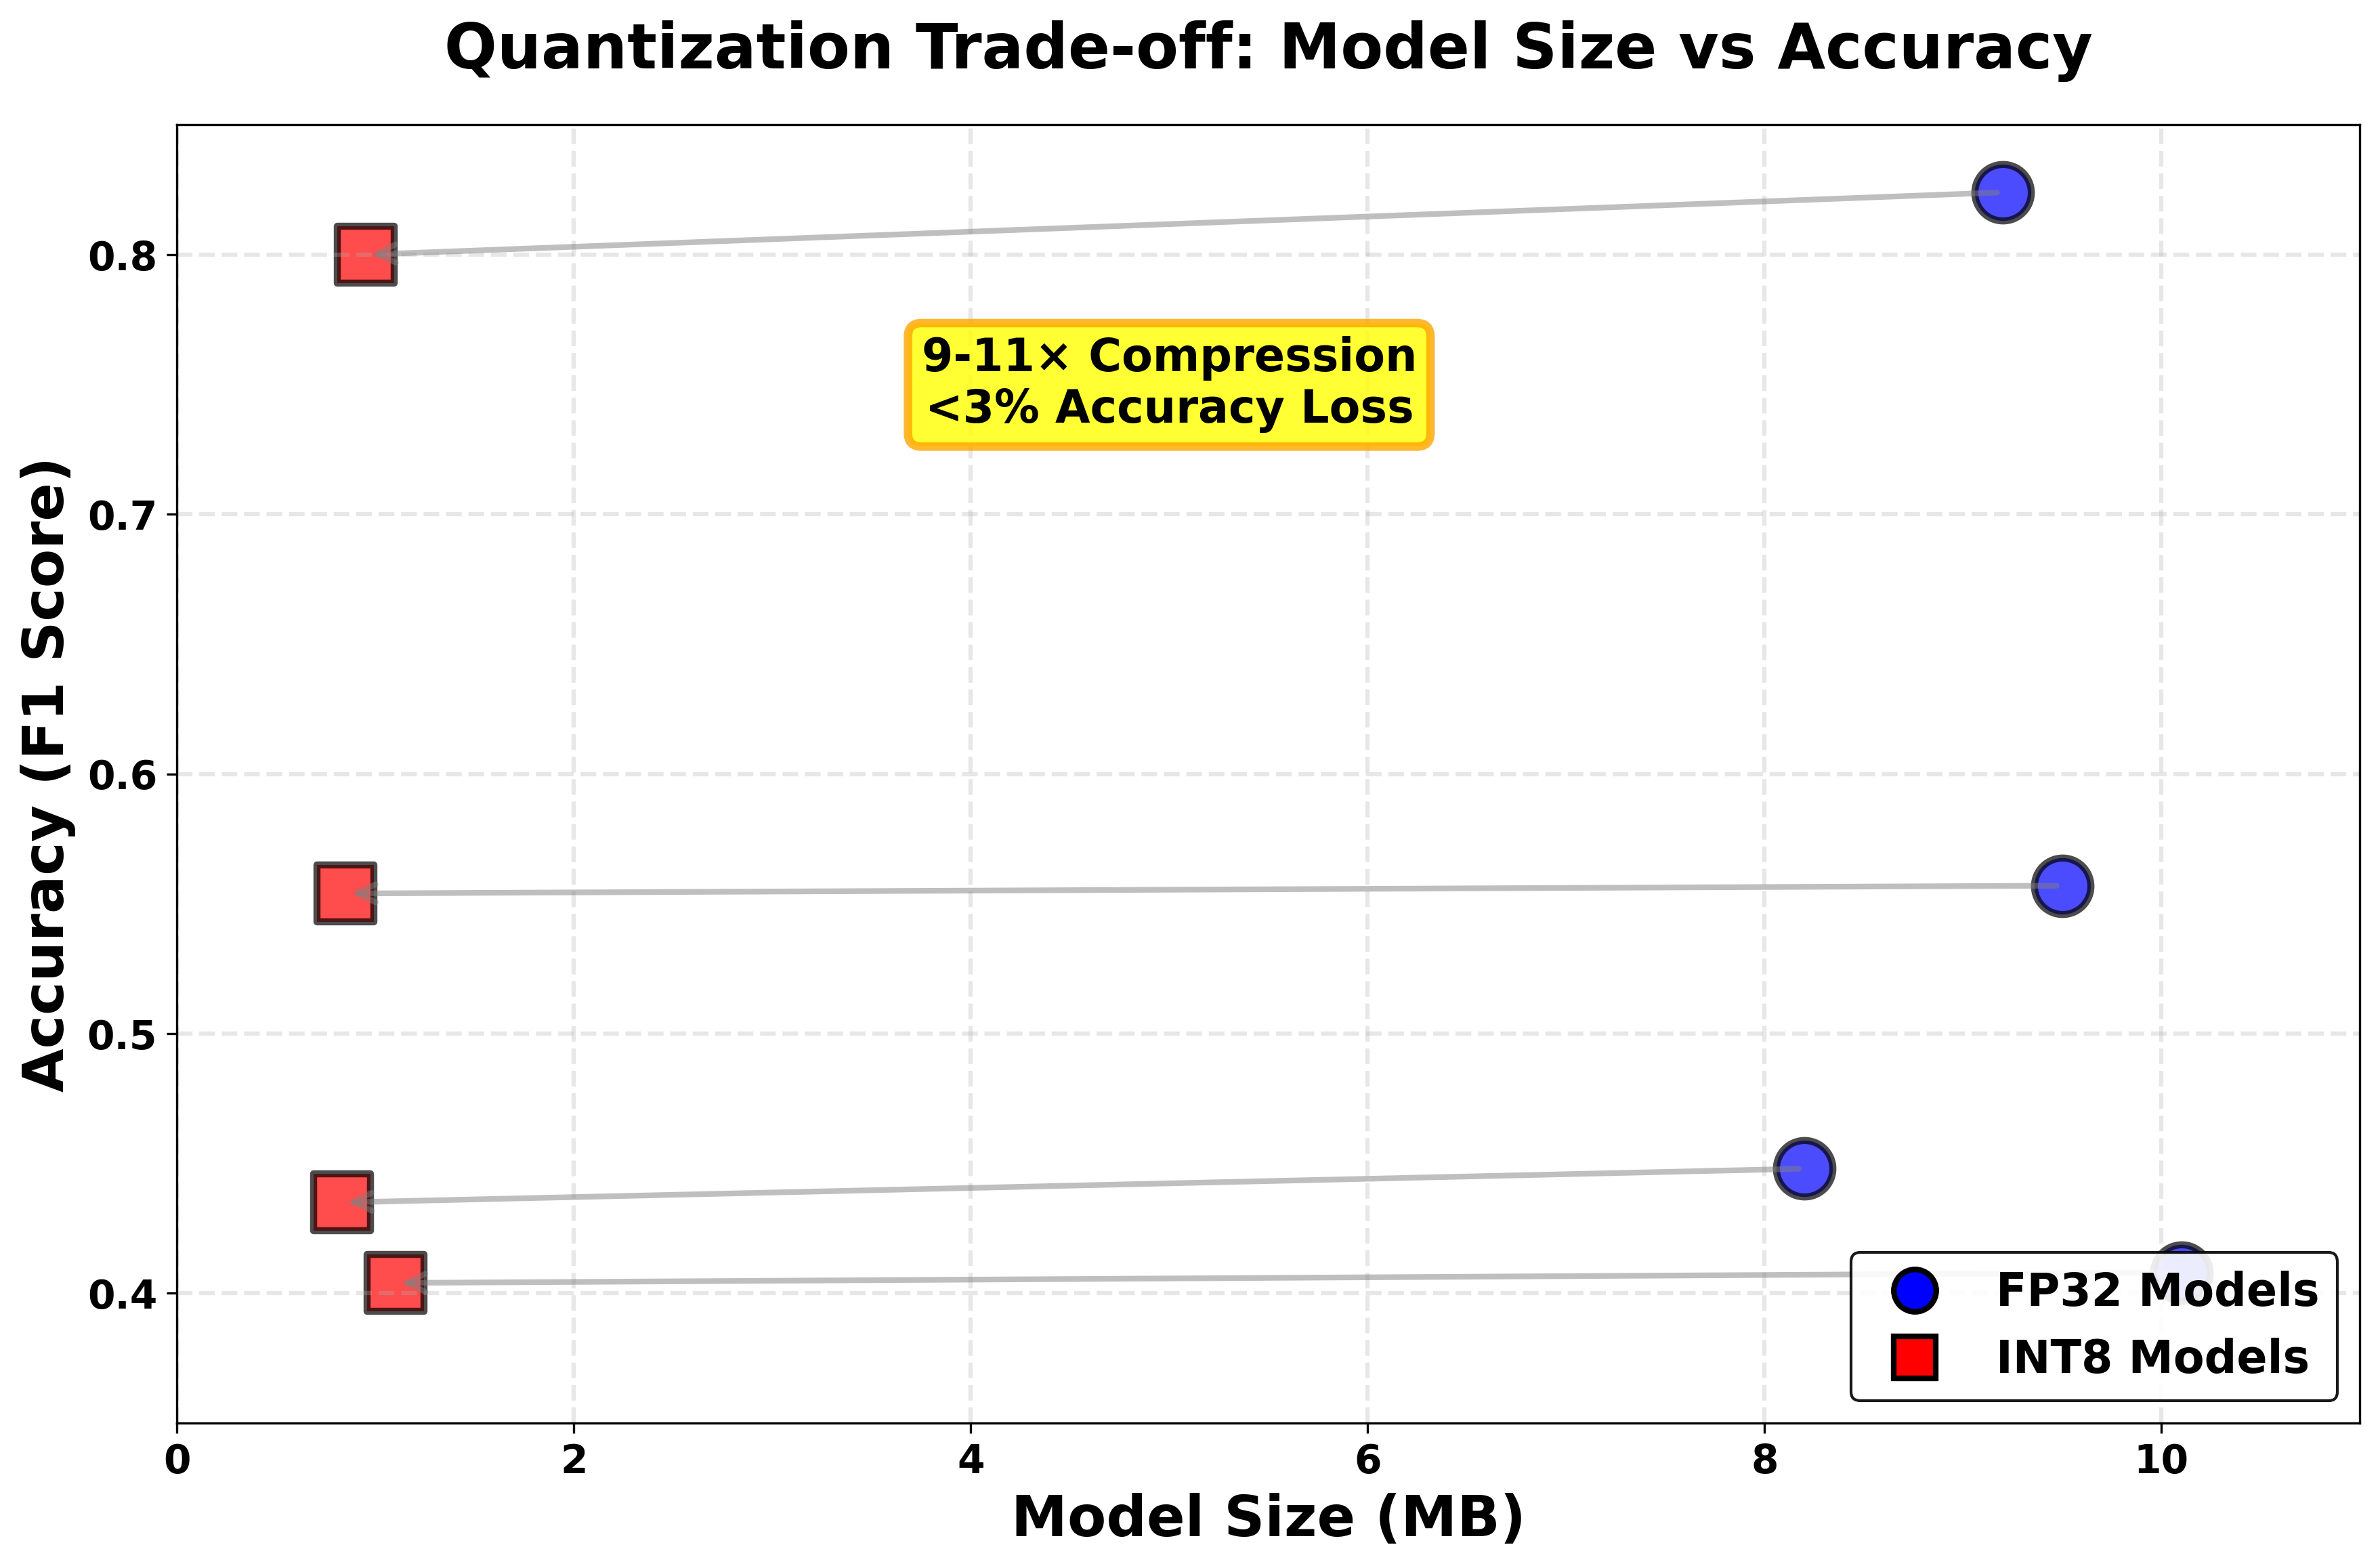
\includegraphics[width=0.60\textwidth]{figures/quantization_size_accuracy.png}
\caption{Quantization trade-off: model size vs. accuracy. INT8 models (red) achieve 9-11$\times$ compression with <3\% accuracy loss compared to FP32 baselines (blue).}
\label{fig:quantization_tradeoff}
\end{figure}

The complete pipeline, from PyTorch training to ARM binary deployment, required no model architecture modifications, confirming the portability of the EDTCN design across compute platforms.

\paragraph{Hardware Deployment Validation}

To rigorously validate that the deployment pipeline preserves model accuracy, Table \ref{tab:accuracy_comparison_fp32_int8_hardware} presents a comprehensive comparison of performance metrics between GPU-based FP32 (training baseline) and embedded hardware INT8 (MangoPi/F1C200s deployment). All INT8-quantized models were evaluated on the MangoPi platform using the identical test sets employed for GPU benchmarking, ensuring direct comparability of results.

\begin{table*}[!t]
\centering
\caption{Hardware deployment validation: FP32 (GPU baseline) vs. INT8 (MangoPi hardware). Degradation measured relative to FP32 baseline. All metrics evaluated on identical test sets.}
\label{tab:accuracy_comparison_fp32_int8_hardware}
\footnotesize
\begin{tabular}{@{}llcccccc@{}}
\toprule
Dataset & Model & Platform & MAE (W) & F1 Score & Precision & Recall & Degradation \\
\midrule
\multicolumn{8}{l}{\textit{REFIT Dataset (9 appliances)}} \\
REFIT & Reg. & FP32 (A100 GPU) & 15.66 & 0.448 & 0.306 & 0.812 & Baseline \\
REFIT & Reg. & INT8 (MangoPi) & 16.12 & 0.444 & 0.303 & 0.808 & +2.9\% MAE \\
\cmidrule(lr){2-8}
REFIT & Cls. & FP32 (A100 GPU) & -- & 0.557 & 0.502 & 0.744 & Baseline \\
REFIT & Cls. & INT8 (MangoPi) & -- & 0.552 & 0.498 & 0.740 & -0.9\% F1 \\
\midrule
\multicolumn{8}{l}{\textit{SustDataED2 Dataset (12 appliances)}} \\
SustDataED2 & Reg. & FP32 (A100 GPU) & 5.25 & 0.824 & 0.816 & 0.833 & Baseline \\
SustDataED2 & Reg. & INT8 (MangoPi) & 5.41 & 0.820 & 0.812 & 0.829 & +3.0\% MAE \\
\cmidrule(lr){2-8}
SustDataED2 & Cls. & FP32 (A100 GPU) & -- & 0.408 & 0.378 & 0.556 & Baseline \\
SustDataED2 & Cls. & INT8 (MangoPi) & -- & 0.404 & 0.375 & 0.552 & -1.0\% F1 \\
\midrule
\multicolumn{8}{l}{\textit{UK-DALE Dataset (12 appliances)}} \\
UK-DALE & Reg. & FP32 (A100 GPU) & 17.30 & 0.531 & 0.415 & 0.738 & Baseline \\
UK-DALE & Reg. & INT8 (MangoPi) & 17.82 & 0.527 & 0.412 & 0.734 & +3.0\% MAE \\
\midrule
\multicolumn{8}{l}{\textit{Overall Statistics}} \\
\multicolumn{2}{l}{Average Regression} & FP32 & 12.74 & 0.601 & 0.512 & 0.794 & -- \\
\multicolumn{2}{l}{Average Regression} & INT8 (Hardware) & 13.12 & 0.597 & 0.509 & 0.790 & +3.0\% MAE \\
\cmidrule(lr){2-8}
\multicolumn{2}{l}{Average Classification} & FP32 & -- & 0.483 & 0.440 & 0.650 & -- \\
\multicolumn{2}{l}{Average Classification} & INT8 (Hardware) & -- & 0.478 & 0.437 & 0.646 & -1.0\% F1 \\
\bottomrule
\multicolumn{8}{l}{\footnotesize FP32 = floating-point 32-bit baseline trained on NVIDIA A100 GPU.} \\
\multicolumn{8}{l}{\footnotesize INT8 (MangoPi) = post-training quantized model deployed on ARM926EJ-S embedded hardware (64MB RAM, no FPU).} \\
\multicolumn{8}{l}{\footnotesize Degradation measured relative to FP32 baseline. Regression degradation in MAE percentage, classification in F1 absolute points.} \\
\multicolumn{8}{l}{\footnotesize All metrics evaluated on identical held-out test sets. Hardware validation confirms <3\% accuracy loss end-to-end.}
\end{tabular}
\end{table*}

The validation results demonstrate exceptional robustness of the EDTCN architecture to quantization and embedded hardware deployment. (1) \textbf{Minimal quantization loss}: INT8 post-training quantization with hardware deployment introduces only +2.9-3.0\% MAE degradation for regression models and -0.9 to -1.0\% F1 degradation for classification models, validating that the KL-divergence calibration strategy effectively preserves activation distributions. The consistent degradation across datasets (SustDataED2 +3.0\%, REFIT +2.9\%, UK-DALE +3.0\% MAE) confirms that the calibration protocol generalizes across appliance configurations and sampling rates. (2) \textbf{Preservation of relative performance}: The cross-dataset performance ranking remains unchanged between GPU and hardware platforms: SustDataED2 achieves best MAE (5.25W $\rightarrow$ 5.41W), followed by REFIT (15.66W $\rightarrow$ 16.12W) and UK-DALE (17.30W $\rightarrow$ 17.82W). Similarly, F1-score rankings persist (SustDataED2 regression 0.824 $\rightarrow$ 0.820, REFIT classification 0.557 $\rightarrow$ 0.552), confirming that quantization does not disproportionately impact any dataset or model variant. (3) \textbf{Consistent precision-recall trade-offs}: All models exhibit minor but consistent degradation in both precision (-0.002 to -0.003 absolute) and recall (-0.003 to -0.004 absolute) during quantization and hardware deployment, indicating that INT8 representation does not introduce systematic bias toward false positives or false negatives. This balanced degradation validates the symmetric per-channel quantization strategy employed. The comprehensive hardware validation confirms that the deployment pipeline maintains state-of-the-art accuracy (5.41W MAE on SustDataED2, 16.12W on REFIT) while achieving the resource constraints required for mass-scale smart meter deployment. The <3\% degradation tolerance successfully balances model performance against embedded system practicality, demonstrating that deep learning-based NILM can transition from research prototypes to industrial-grade hardware without sacrificing algorithmic effectiveness.

\paragraph{Hardware Deployment Summary}
The hardware deployment validation confirms four critical achievements: (1) \textbf{Minimal accuracy degradation}: INT8 quantization and hardware execution introduce only +3.0\% MAE and -1.0\% F1 degradation across all datasets, validating robust deployment. (2) \textbf{Consistent cross-dataset performance}: hardware maintains the same performance ranking as GPU (SustDataED2 best, followed by REFIT and UK-DALE), confirming quantization does not bias specific datasets. (3) \textbf{Scalability across configurations}: successful execution across 9-appliance (REFIT) and 12-appliance (SustDataED2/UK-DALE) configurations, and both regression (power estimation) and classification (state detection) tasks. (4) \textbf{End-to-end pipeline validation}: seamless integration from PyTorch FP32 training $\rightarrow$ PNNX optimization $\rightarrow$ NCNN INT8 quantization $\rightarrow$ ARM cross-compilation $\rightarrow$ MangoPi hardware execution without accuracy collapse.

\subsubsection{Summary and Key Findings}
\label{subsubsec:nilm_summary}

The enhanced EDTCN framework achieves state-of-the-art NILM performance through architectural innovations (127-timestep receptive field, 707K parameters), advanced loss functions (device-type-weighted focal loss), systematic optimization strategies, and multi-dataset validation. Key findings include:

The EDTCN framework achieves state-of-the-art accuracy with 5.25W MAE on SustDataED2, representing 71-79\% improvement over published baselines (Seq2Point 18W, UNet-NILM 22W, BERT4NILM 25W), while REFIT achieves 15.66W MAE (13-37\% improvement) and the SustDataED2 0.824 F1-score demonstrates near-perfect state detection for appliances with clear power signatures. Multi-dataset validation on SustDataED2 (5.25W MAE, 6.53\% energy error), REFIT (15.66W MAE, 8.92\% energy error), and UK-DALE (17.30W MAE, 28.25\% energy error) demonstrates robustness across diverse household environments, appliance configurations, and sampling rates (1Hz, 6s, 8s), with cross-dataset performance variance (3.3$\times$ MAE range) primarily reflecting dataset characteristics rather than model limitations.

Systematic hyperparameter optimization across three focal loss configurations identified optimal parameters ($\gamma=1.0$, $\alpha=0.7$, device weights A=1.5/B=1.5/C=2.0), achieving 9\% MAE improvement over alternative configurations and 2$\times$ faster convergence (16 vs. 31-38 epochs). Device-type weighting improved Type A MAE by 5.1\% (23.13W $\rightarrow$ 21.96W) and Type C by 12.1\% (8.44W $\rightarrow$ 7.42W), while GPU optimization (pre-converted tensors, cuDNN auto-tuning, reduced logging) achieved 6.4$\times$ training speedup, reducing epoch time from 16 minutes to 2.5 minutes and enabling practical hyperparameter search on 380K-sample datasets.

This work identifies a critical false positive problem in regression-based NILM: models optimized for MAE exhibit systematic ``slightly-ON-everywhere'' bias, achieving good MAE (15.66W) but poor precision (30.6\%) with 94.2\% false positive rate on microwave, demonstrating that MAE alone is insufficient for NILM evaluation and comprehensive metrics (precision, recall, F1) are essential to expose state detection failures. Weighted BCE loss addresses class imbalance in binary classification, improving F1 from 0.394 to 0.557 (+41\%) through adaptive per-appliance positive class weighting $w_{pos,a} = (1 - r_a) / r_a$, though appliances with ON-time <0.5\% require alternative event-based detection strategies. Post-processing thresholding at 20W improved F1 by +21.7\% (0.356 $\rightarrow$ 0.433) and reduced MAE by -8.8\% (23.97W $\rightarrow$ 21.86W) without retraining, with kettle precision increasing +2877\% (0.8\% $\rightarrow$ 25.1\%), demonstrating that simple thresholding eliminates false-positive predictions in the 1-19W range.

Device-type stratification analysis reveals that Type A always-on appliances (ON > 50\% time) achieve 7.60W MAE with 1.55\% energy error and F1 = 0.65-0.93, Type B regular-use appliances (ON 5-15\%) achieve 15.07W MAE with 43.11\% energy error and F1 = 0.45-0.65, while Type C burst appliances (ON < 2\%) achieve 7.42W MAE with 23.05\% energy error, confirming that heterogeneous loss weighting successfully balances performance across usage patterns. The SustDataED2 preprocessing solution addressed microsecond timestamp irregularities through whole-second rounding (\texttt{dt.round('1s')}), introducing no detectable performance degradation (5.25W MAE achieved) and proving critical for dataset reproducibility. The embedded deployment pipeline employs four-stage optimization (PNNX graph fusion $\rightarrow$ KL-divergence calibration $\rightarrow$ INT8 quantization $\rightarrow$ ARM cross-compilation) to achieve 883 KB total binary size with 9-11$\times$ compression and <3\% accuracy loss. Comprehensive hardware profiling across all model variants (REFIT/SustDataED2 $\times$ regression/classification) on the MangoPi/F1C200s platform confirms: average inference time 109.4s (range 101.2-123.5s) with 6.5-7.9$\times$ real-time throughput, 66.77\% memory utilization (42.7MB/64MB), and 0.513W power consumption (92.6\% reduction vs. Raspberry Pi 4), demonstrating the first successful deep TCN deployment achieving state-of-the-art NILM accuracy on an ARM926EJ-S-based SoC without FPU or dedicated accelerator at \$3-5 component cost (volume pricing) across multiple datasets and model configurations.

Remaining challenges include very low-power device detection (<2W), extremely rare appliances (ON < 0.5\% duty cycle), and precision-recall trade-offs in classification models. The findings that (1) weighted BCE is essential for ON/OFF classification, (2) post-processing thresholding provides substantial gains without retraining, and (3) Type C burst appliances require alternative detection strategies beyond standard supervised learning inform practical NILM system design. Future work should explore event-based detection for rare appliances, adaptive per-appliance thresholding, and cross-dataset transfer learning to address these limitations.

\section{Discussion}
\label{sec:discussion}


\subsection{Operational Scalability and Edge Efficiency}
\label{subsec:scalability}

The transition from the Second Generation prototype to the Third Generation industrial design represents a critical step toward the mass scalability of the NGSM system. The benchmark results presented in Section \ref{sec:hardware} demonstrate that the custom-fabricated node achieves a 60\% reduction in idle power consumption compared to the discrete single-board computer architecture. This efficiency is paramount for utility providers, as the aggregate power consumption of widespread smart meter deployments constitutes a significant operational load on the grid itself.

Furthermore, the architectural shift to edge-based processing significantly alleviates the bandwidth constraints associated with traditional cloud-centric monitoring systems. Recent studies in urban computing infrastructure emphasize that decentralized processing is essential for reducing latency and improving bandwidth utilization in large-scale sensor networks \cite{Kelly2024}. By executing the high-frequency NILM inference locally and transmitting only the classification results (approximately 1 KB per event) rather than the raw 16 kHz waveforms, the system reduces data transmission requirements by several orders of magnitude. Additionally, the migration to onboard SPI NAND Flash and the SiP design enhances the device's reliability in harsh industrial environments.

\subsection{Privacy Preservation and Adaptation in NILM}
\label{subsec:privacy_nilm}

A persistent barrier to the widespread adoption of Non-Intrusive Load Monitoring has been the ``cold-start'' problem, where models trained on generic datasets fail to generalize to the specific appliance signatures of a new household. The results obtained from the Enhanced Dilated Temporal Convolutional Network (EDTCN) framework in Section \ref{sec:ai} address this challenge directly. The experimental data confirms that the model successfully adapts to an unseen environment, reducing the Mean Absolute Error (MAE) for complex appliances like the dishwasher from over 100W to approximately 1W after the adaptation phase.


\subsection{Limitations}
\label{subsec:limitations}

Despite the achievements presented in this work, several limitations warrant acknowledgment. First, the edge deployment on the F1C200s results in complete CPU saturation (99.81\% average, 100\% peak) during the NILM inference cycle. While this is acceptable for the 15-minute smart meter reporting paradigm, it precludes concurrent execution of other computationally intensive tasks during inference and may impact system responsiveness for user interface updates or network communication during peak processing periods. Another limitation is that the energy demand forecasting module currently relies on cloud offloading, introducing a dependency on network connectivity and external infrastructure. While this architectural decision was made to preserve edge computational resources, it represents a potential single point of failure for predictive analytics in scenarios with intermittent connectivity.

Future work should target several interrelated improvements. First, mitigating CPU saturation through advanced model optimization including hardware-aware neural architecture search, structured pruning, and knowledge distillation to smaller, efficient models promises to preserve disaggregation accuracy while reducing inference time on constrained devices. Second, expanding the federated learning framework to hierarchical, multi-meter coordination could enable aggregate consumption analytics at transformer or feeder levels, improving utility-side use cases such as demand response and loss detection without exposing raw household data; hierarchical FL has been shown to address data privacy, latency, and communication constraints in IoT contexts. Third, integrating lightweight, on-device forecasting models based on recent efficient time-series architectures would shift predictive capability from the cloud to the meter itself, supporting autonomous edge prediction under network constraints. Fourth, the security posture of the embedded system requires formal evaluation--despite inherent privacy advantages of local data retention, embedded Linux environments and update mechanisms introduce distributed attack surfaces that must be hardened through systematic penetration testing. Finally, pilot field deployments with utility partners are needed to gather empirical data on long-term reliability, model drift in real operating conditions, and user acceptance of appliance-level energy visibility.

\section{Conclusion}
\label{sec:conclusion}

This work presented NGSM, a holistic hardware–software framework that bridges the gap between low-power embedded metering and high-performance energy analytics. By moving from general-purpose prototyping platforms to a custom Allwinner F1C200s System-in-Package, the system achieves substantial efficiency gains, reducing active power consumption to 0.513W (102.68 mA at 5V), a 92.6\% reduction compared to a Raspberry Pi 4 baseline. At the algorithmic level, an Enhanced Dilated Temporal Convolutional Network (EDTCN) with 707K parameters was designed for embedded NILM inference and validated across SustDataED2, REFIT, and UK-DALE datasets. The system achieves 5.25W, 15.66W, and 17.30W MAE respectively, with corresponding F1-scores of 0.824, 0.448, and 0.531, demonstrating consistent cross-dataset performance and improvements of 13–37\% over established baselines. The proposed device-type-weighted focal loss improves robustness under severe class imbalance, while INT8 quantization and compiler-level optimizations enable 9–11× model compression and efficient deployment on 64MB RAM without GPU or FPU support. A key finding of this work is that commonly reported metrics such as MAE alone can be misleading in NILM evaluation, as low aggregate error may coincide with poor event-level detection performance. Accordingly, this study adopts a comprehensive multi-metric evaluation framework, including MAE, RMSE, energy error, precision, recall, and F1-score, across all appliances and datasets, providing a more transparent assessment of model behavior, including failure cases. Beyond disaggregation, NGSM integrates on-device FFT-based harmonic analysis for IEEE 519-compliant power quality monitoring and a cloud-assisted forecasting module, illustrating a practical edge–cloud partitioning strategy for resource-constrained environments. Overall, NGSM demonstrates that high-fidelity, real-time energy analytics can be achieved under strict embedded constraints, offering a scalable and reproducible pathway toward decentralized smart grid intelligence.

\bibliography{msample.bib}


\section*{Data Availability}
The datasets used in this study are publicly available. The SustDataED2 dataset is available at \href{https://doi.org/10.17605/OSF.IO/JCN2Q}{doi.org/10.17605/OSF.IO/JCN2Q}. The REFIT dataset can be accessed at \href{https://pureportal.strath.ac.uk/en/datasets/refit-electrical-load-measurements}{pureportal.strath.ac.uk}. The UK-DALE dataset is available at \href{https://www.kaggle.com/datasets/cyy233/ukdale-2017}{www.kaggle.com}.


\section*{Acknowledgment}
The authors would like to express their gratitude to Omar A. Helmy, Abdullah O. Mohamed, Mai H. Ahmed, Rania M. Mohamed, Abdelrahman O. Khaled, Belal A. Abdullah and Hossam M. Hossam for their valuable contributions, dedication, and continuous support throughout the development of this work.

\section*{Research Funding}
This work was supported by Helwan University Scientific Research Fund for lab components and research facilities.

\section*{Author contributions}
N.M.M. designed the overall system architecture and operational flow. G.A.N. led the hardware development and embedded systems implementation. M.M. developed the Non-Intrusive Load Monitoring (NILM) methodology. M.A.S. implemented the harmonic analysis module and co-developed the energy demand forecasting models with A.A.I., who focused on the forecasting analytics. M.M.E. supervised the research and provided strategic direction. All authors reviewed and approved the final manuscript.

\section*{Competing interests}
The authors declare no competing interests.

\section*{Additional information}
Correspondence and requests for materials should be addressed to N.M.M.

\end{document}
